%\documentclass[]{siamart190516}
%\documentclass{book}
\documentclass[hidelinks,notitlepage]{book}
%\usepackage{siamart190516}

\usepackage{graphicx}
\graphicspath{ {./images/} }

\usepackage{amsfonts}
\usepackage{graphicx}
\usepackage{epstopdf}
\usepackage{float}
\usepackage{courier}
\usepackage{hyperref}
\usepackage{algorithm}
\usepackage{algorithmic}
\usepackage{authblk}
\usepackage{caption}
\usepackage{listings}
\usepackage{color}
\usepackage[frak=esstix]{mathalpha}
\usepackage{array}
\usepackage{booktabs}
\usepackage{subcaption}


\usepackage{epstopdf,epsfig}    
\epstopdfsetup{outdir=./}
\usepackage[section]{placeins}

\usepackage{amsopn}
\DeclareMathOperator{\diag}{diag}

\usepackage{amsmath}
\DeclareMathOperator*{\argmax}{argmax}
\DeclareMathOperator*{\argmin}{argmin}

% Set letter size since the SIAM package uses a small page size.
\usepackage[letterpaper]{geometry}

% This provides \cref
\usepackage[]{cleveref}

\DeclareGraphicsExtensions{.eps,.pdf,.png,.jpg}


% Add a serial/Oxford comma by default.
\newcommand{\creflastconjunction}{, and~}

\newcommand{\R}{\mathbb{R}}

\graphicspath{ {./images/} }

% Define "struts" as suggested by Claudio Beccari in
% a piece in TeX and TUG News, Vol. 2, 1993.
%\newcommand\Tstrut{\rule{0pt}{2.6ex}}       % "top" strut
%\newcommand\Bstrut{\rule[-0.9ex]{0pt}{0pt}} % "bottom" strut
%\newcommand{\TBstrut}{\Tstrut\Bstrut} % top&bottom struts


% Title. 
\title{Numerically Solving Ordinary Differential Equations}
\author{Stuart D. Brorson}
\affil{Northeastern University}


\begin{document}
\maketitle

These are class notes meant to accompany MATH7205, Numerical Analysis 2 at Northeastern University.   This document introduces techniques useful to solve ODEs numerically.  It also motivates the techniques, explains how they work, and examines some of the pitfalls which accompany the techniques.  The student is expected to have a good grasp of calculus, ODEs, and linear algebra, and also be familiar with numerical methods for solving linear and nonlinear systems of equations.


\newpage

\tableofcontents

\mainmatter
\chapter{Introduction}
\section{Solving ordinary differential equations}
Solving ordinary differential equations (ODEs) is a major focus of numerical computing.  We start by considering first-order ODEs of the form
\begin{equation}
\label{eq:SimpleODE}
y' = f(t, y) 
\end{equation}
Where $y(t)$ is the unknown (i.e. the thing we want to find), and $t$ is the independent variable.  When dealing with such an ODE, we usually think of $t$ as
time, and $y$ as something depending upon time, like the population of an animal species or the voltage of a node in an electronic circuit.  
Equation \cref{eq:SimpleODE} says that the way $y$ changes in time depends upon some function $f$.  
In this booklet, we assume the function $f$ is smooth and well-behaved, and that it is easily calculable in a computer program.

One may write down solutions to \cref{eq:SimpleODE}, but to get a \textit{unique} solution an additional piece of information is required:  An initial condition.  That is, we need to know something about $y(t)$ at one point in time so we can select one individual solution from all possible solutions which satisfy \ref{eq:SimpleODE}.  One traditionally uses a value for $y(t)$ at time $t=0$ as the initial condition, but other choices are also possible (but uncommon). 

Here's a very basic example.  Consider the ODE
\begin{equation}
\label{eq:BasicODE}
y' = a y
\end{equation}
You likely encountered this ODE early in your mathematical career, and you know the solution by heart:
\begin{equation}
\label{eq:BasicODESoln}
y(t) = C e^{a t}
\end{equation}
where $C$ is some constant.  The solution \cref{eq:BasicODESoln} obviously satisfies equation \cref{eq:BasicODE}, but it is not useful in practice as the solution to the equation.  Why?  The reason is that there are an infinite number of possible solutions depending upon the value of $C$ chosen.  That is, \cref{eq:BasicODESoln} defines a family of solutions, but in a real, practical problem we only want one of those solutions.  For example, how would you make a plot of \cref{eq:BasicODESoln}?  The answer is, you can't, until you chose a specific value of $C$.  

In a practical problem, you usually know the value of your function at a start-point in time, almost always at $t = 0$.  Call that value $y_0$.  In this case, the specific solution which satisfies \cref{eq:BasicODE} and also satisfies $y(t=0) = y_0$ is
\begin{equation}
y(t) = y_0 e^{a t}
\end{equation}
The point is that numerically solving an ODE requires two pieces of information:  1.  The ODE itself, and 2.  An initial condition.  The initial value picks one solution out of the entire family of solutions which satisfy \cref{eq:BasicODE}.  The concept is shown in \cref{fig:ODEFlowLines}
\begin{figure}[tbh]
	\centering
	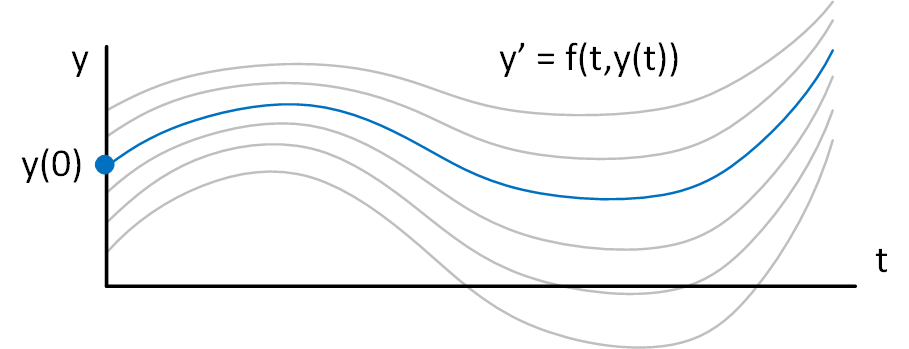
\includegraphics[width=0.8\columnwidth]{ODEFlowLines.png}
	\caption{The ODE $y' = f(t,y)$ is satisfied by a family of curves.  An initial condition $y(0)$ is required to pick out one of the solutions for numerical simulation. }
	\label{fig:ODEFlowLines}
\end{figure}
Such a problem is called an "initial value problem" (IVP) to distinguish it from other types of differential equations (which we will encounter later in the class).  "Initial value problem" simply means we know the beginning (initial) value of $y$, and want to find its behavior as we move forward in time.  Once the equation \ref{eq:SimpleODE} and an initial condition for $y$ are specified, then we have all the information required to find a unique solution $y(t)$ numerically.  

Methods to find numerical solutions IVPs are the focus of this booklet.  As a matter of nomenclature, we generally say "solve the ODE", or "solve the IVP".  This means we compute the function $y(t)$ starting from time $t=0$ to some point in the future, $t_{end}$.  Another way to say the same thing is we "integrate the ODE", or "integrate the IVP".  When speaking of ODEs, "integrate" means the same thing as "solve".

\section{Sampled functions}
In mathematics we become familiar with the notion of a function.  Consider the simplest case of a function $y(t)$ which takes a real scalar $t$ and returns a real scalar value $y(t)$.  This is frequently written formally as $y:\mathbb{R}\rightarrow \mathbb{R}$.  This means, take any arbitrary real number $t$, plug it into $y$, and out will come a new real number $y(t)$.  The important idea to glean from this is that the function is like a machine into which one can input any $t$ and expect to get an output.  That is, the function is defined on every real number $t$.

Unfortunately, when working on real data using a computer this nice abstraction doesn't always hold.  Rather, it is very common for us to have only certain, discrete points $t_n$ where the function is defined.  Digital audio is a simple example:  the sounds we hear with our ear are related to the sound pressure waves moving our eardrums.  The sound pressure has a value for every point in time.  But when processing audio using a computer the sound pressure is sampled at regular, discrete times and turned into numbers representing the sound pressure at each sample time.  This process is often referred to as "discretization", meaning that the continuously-defined $y(t)$ is replaced by a set of discrete samples $y_n$.  This is depicted in \cref{fig:SampledFcn}, which shows the relationship of a continuous-time function and its discrete-time (discretized) replacement.
\begin{figure}[tbh]
	\centering
	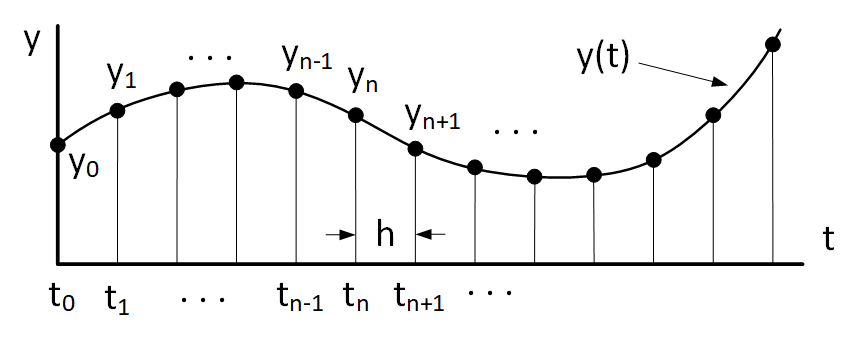
\includegraphics[width=0.8\columnwidth]{SampledFcn.png}
	\caption{A sampled function.  The continuous-time version of the function is $y(t)$.  Sampling replaces $y(t)$ with samples taken at discrete times, $t_n$.  The samples $y_n$ may be handled by the computer as a vector or list of values.  In the case shown here the function is sampled at evenly-spaced intervals separated by $h$.  Evenly-spaced samples are the most frequent case -- for example, digital audio commonly samples an input sound signal with a period $h$ of about 22.7usec (44.1kHz sampling rate).}
	\label{fig:SampledFcn}
\end{figure}
It turns out that the ODE solvers we will study all work with sampled functions.  That is, the solvers compute the solution $y(t)$ at a sequence of discrete time values $t_n$ similar to the situation shown in \cref{fig:SampledFcn}.  The output of the solver will be a vector of discrete values $y_n$ representing samples of the actual, underlying continuous function $y(t)$.

Here is an implementation hint when you write programs processing sampled functions:  The sampled function itself is generally represented by a vector, $y_n$.  This is the object your algorithm will use during its work.  On top of $y_n$ I recommend also carrying around a vector representing the sample times, $t_n$, in your program.  Having your sample times readily accessible can help decrease confusion when you want to plot $y_n$ vs. time, for example.  For moderately sized vectors, the extra memory required to hold $t_n$ is a small price to pay to keep confusion at a minimum while writing your code.


\section{Differentiation on the computer}
Next before diving into solving \cref{eq:SimpleODE} we need to review how differentiation is done on the computer.  To start, recall the definition of the derivative of $y(t)$ which you probably learned in high school:
\begin{equation}
\label{eq:DiffDef}
\frac{d y}{d t} = 
\lim_{{\Delta t}\to 0} 
\frac{y(t + \Delta t) - y(t)}{\Delta t}
\end{equation}
In doing numerical computation, we can't represent the limiting transition $\lim_{{\Delta t}\to 0}$ -- our data is usually discrete (e.g. a sampled function).  More importantly, floating point numbers don't smoothly transition to zero -- there is no "infinitesimally small but nonzero" number representable on a computer.  Instead, we use the definition \cref{eq:DiffDef} to form an approximation to the derivative as
\begin{equation}
\label{eq:ForwardDiffApprox}
\frac{d y}{d t} \approx
\frac{y(t + h) - y(t)}{h}
\end{equation}
where $h$ is a small number.  This is called the "forward difference" approximation of the derivative.

\subsection{First derivatives from Taylor's series}
\label{sect:ForwardDiff}
It's easy to write down the approximation \cref{eq:ForwardDiffApprox} by remembering the high school definition of a derivative.  However, we gain some appreciation for the accuracy of approximating derivatives by deriving them using Taylor series expansions.  Suppose we know the value of a function $y$ at the time $t$ and want to know its value at a later time $t+h$. How to find $y(t+h)$?  The Taylor's series expansion says we can find the value at the later time by
\begin{equation}
\label{eq:ForwardTaylorsExpansion}
y(t+h) = y(t) 
+ h \frac{d y}{d t} \biggr\rvert_{t}
+ \frac{h^2}{2} \frac{d^2 y}{d t^2} \biggr\rvert_{t}
+ \frac{h^3}{6} \frac{d^3 y}{d t^3} \biggr\rvert_{t}
+ O(h^4)
\end{equation}
The notation $O(h^4)$ means that there are terms of power $h^4$ and above in the sum, but we will consider them details which we can ignore.  

We can rearrange \cref{eq:ForwardTaylorsExpansion} to put the first derivative on the LHS, yielding
\begin{equation}
\nonumber
\frac{d y}{d t} \biggr\rvert_{t} =
\frac{y(t+h) - y(t)}{h}
- \frac{h}{2} \frac{d^2 y}{d t^2} \biggr\rvert_{t}
- \frac{h^2}{6} \frac{d^3 y}{d t^3} \biggr\rvert_{t}
- O(h^4)
\end{equation}
Now we make the assumption that $h$ is very small, so we can throw away terms of order $h$ and above from this expression.  With that assumption we get
\begin{equation}
\nonumber
y(t+h) \approx y(t) 
+ h \frac{d y}{d t} \biggr\rvert_{t}
\end{equation}
which can be rearranged to give
\begin{equation}
\label{eq:ForwardDiffApprox1}
\frac{d y}{d t} \approx
\frac{y(t + h) - y(t)}{h}
\end{equation}
i.e. the same forward difference expression as found in \cref{eq:ForwardDiffApprox} earlier.  However, note that to get this approximation we threw away all terms of order $h$ and above.  This implies that when we use this approximation we incur an error!  That error will be on the order of $h$.  In the limit $h \rightarrow 0$ the error disappears but since computers can only use finite $h$, there will always be an error in our computations, and the error is proportional to $h$.  We express this concept by saying the error scales as $O(h)$.

Using Taylor's series expansions we can discover other results.  Consider sitting at the time point $t$ and asking for the value of $y$ at time $t - h$ in the past. In this case, we can write an expression for the past value of $y$ as
\begin{equation}
\label{eq:BackwardTaylorsExpansion}
y(t-h) = y(t) 
- h \frac{d y}{d t} \biggr\rvert_{t}
+ \frac{h^2}{2} \frac{d^2 y}{d t^2} \biggr\rvert_{t}
- \frac{h^3}{6} \frac{d^3 y}{d t^3} \biggr\rvert_{t}
+ O(h^4)
\end{equation}
Note the negative signs on the odd-order terms.  Similar to the forward difference expression above, it's easy to rearrange this expression and then throw away terms of $O(h)$ and above to get a different approximation for the derivative,
\begin{equation}
\label{eq:BackwardDiffApprox}
\frac{d y}{d t} \approx
\frac{y(t) - y(t-h)}{h}
\end{equation}
This is called the "backward difference" approximation to the derivative.  Since we threw away terms of $O(h)$ and above, this expression for the derivative also carries an error penalty of $O(h)$.

Now consider forming difference between Taylor series \cref{eq:ForwardTaylorsExpansion} and \cref{eq:BackwardTaylorsExpansion}.  When we subtract one from the other we get
\begin{equation}
\label{eq:TaylorsExpansionDifference}
\nonumber
y(t+h) - y(t-h) = 
2 h \frac{d y}{d t} \biggr\rvert_{t}
+ 2 \frac{h^3}{6} \frac{d^3 y}{d t^3} \biggr\rvert_{t}
+ O(h^5)
\end{equation}
This expression may be rearranged to become
\begin{equation}
\nonumber
\frac{d y}{d t} \biggr\rvert_{t} =
\frac{y(t+h) - y(t-h)}{2 h}  
-  \frac{h^2}{6} \frac{d^3 y}{d t^3} \biggr\rvert_{t}
+ O(h^4)
\end{equation}
Now if we throw away terms of $O(h^2)$ and above, we get the so-called "central difference" approximation for the derivative,
\begin{equation}
\label{eq:CentralDifferenceApproximation}
\frac{d y}{d t} \biggr\rvert_{t} \approx
\frac{y(t+h) - y(t-h)}{2 h}  
\end{equation}
Note that to get this expression we discarded $O(h^2)$ terms.  This implies that the error incurred upon using this expression for a derivative is $O(h^2)$.  Since we usually have $h \ll 1$, the central difference error $O(h^2)$ is smaller than the $O(h)$ incurred when using either the forward or backward difference formulas.  That is, the central difference expression \cref{eq:CentralDifferenceApproximation} provides a more accurate approximation to the derivative than either the forward or the backward difference formulas, and should be your preferred derivative approximation when you can use it.

In each of these derivations we threw away terms of some order $p$ (and above).  Discarding terms of order $p$ and above means we no longer have a complete Taylor series.  This operation is called "truncation", meaning we have truncated (chopped off) the remaining terms of the full Taylor series.  The error incurred by this operation is therefore called "truncation error".  

\subsection{Second derivatives from Taylor's series}
We can also get an approximation for the second derivative from expressions \cref{eq:ForwardTaylorsExpansion} and \cref{eq:BackwardTaylorsExpansion}.  This time, form the sum of the two expressions to get
\begin{equation}
\nonumber
\label{eq:TaylorsExpansionSum}
y(t+h) + y(t-h) = 2 y(t)
+ 2 \frac{h^2}{2} \frac{d^2 y}{d t^2} \biggr\rvert_{t}
+O(h^4)
\end{equation}
This may be rearranged to get an expression for the second derivative,
\begin{equation}
\nonumber
\frac{d^2 y}{d t^2} \biggr\rvert_{t} =
\frac{y(t+h) -2 y(t) + y(t-h)}
{h^2}
-O(h^2)
\end{equation}
If we drop the $O(h^2)$ term, we get the approximation to the second derivative,
\begin{equation}
\label{eq:SecondDerivative}
\frac{d^2 y}{d t^2} \biggr\rvert_{t} \approx
\frac{y(t+h) -2 y(t) + y(t-h)}
{h^2}
\end{equation}
And since we dropped the $O(h^2)$ term to make this approximation, it means that use of \cref{eq:SecondDerivative} will incur an error of  $O(h^2)$ when using this approximation.

\section{Chapter summary}
Here are the important points made in this chapter:
\begin{itemize}
	\item Solving an ODE numerically needs two pieces of information:  The ODE and an initial condition.  Such problems are called "initial value problems", or IVPs.
	\item As mathematicians, we are used to functions $y(t)$ which accept any continuous value of $t$ and emit a value.  However, when dealing with computers, we must frequently use "sampled functions" in which the continuous $y(t)$ is replaced with samples $y_n$ taken at regular, discrete points in time, $t_n$.  The ODE solvers presented in this booklet fall into this category -- they provide samples of the solution at discrete times, similar to snapshots of the continuous function they try to approximate.
	\item \Cref{tab:FiniteDiffExpressions} summarizes the four different approximations for derivatives we have encountered so far.  There are many more derivative approximations of higher order, and using more terms.  The higher order approximations give better accuracy at the cost of additional complexity.  Higher order approximations are used less frequently than the four shown here.
\end{itemize}

\begin{table}[h]
\begin{center}
	\renewcommand{\arraystretch}{1.5}
	
\begin{tabular}{ |c|c|c|c| } 

	\hline
	 \textbf{Derivative} & \textbf{Method name} & \textbf{Expression} & \textbf{Error order} \\ 
	\hline
	$\frac{d y}{d t}$ & Forward difference & $\frac{y_{n+1}-y_n}{h}$ & $h$ \\ 
	$\frac{d y}{d t}$ & Backward difference & $\frac{y_{n}-y_{n-1}}{h}$  & $h$ \\ 
	$\frac{d y}{d t}$ & Central difference & $\frac{y_{n+1}-y_{n-1}}{2 h}$  & $h^2$ \\ 
	$\frac{d^2 y}{d t^2}$ & Second derivative & $\frac{y_{n+1}-2 y_{n}+y_{n-1}}{h^2}$  & $h^2$ \\ 
	\hline
\end{tabular}
\caption{Commonly used finite difference derivatives.}\label{tab:FiniteDiffExpressions}
\end{center}
\end{table}

%%%%%%%%%%%%%%%%%%%%%%%%%%%%%%%%%%%%%%%%%%%%%%%%%%%%%%%%%%%%%%%%%%%%%%%%%%%%%%%%%%%%%%%%%%%%%%%%%%%%%%%%%%%%%%%%%%%%%%%%%
%%%%%%%%%%%%%%%%%%%%%%%%%%%%%%%%%%%%%%%%%%%%%%%%%%%%%%%%%%%%%%%%%%%%%%%%%%%%%%%%%%%%%%%%%%%%%%%%%%%%%%
\chapter{Forward Euler method}
\section{Forward Euler algorithm}
\label{sect:ForwardEulerMethod}
Now we examine our first ODE solver:  the Forward Euler method.  Here is the problem and the goal:  Given a scalar, first-order ODE,
\begin{equation}
\label{eq:FirstOrderODE}
\frac{d y}{d t} = f(t, y) 
\end{equation}
and an initial condition $y(t=0) = y_0$, find how the function $y(t)$ evolves for all times $t > 0$.  In particular, write down an algorithm which may be executed by a computer to find the evolution of $y(t)$ for all times.

To derive the algorithm, first replace the exact equation with an approximation based on the forward difference derivative to get
\begin{equation}
\label{eq:FwdDiffDerivation}
\frac{y(t + h) - y(t)}{h} \approx f(t, y) 
\end{equation}
Now discretize the equation.  That means we replace our function $y(t)$ defined on continuous $t$ with a sampled function $y_n$ defined on discrete times $t_n$.  That is, $y_n = y(t_n)$.  We also imagine the time step between samples is small, $h = t_{n+1} - t_n$.  In this case, \cref{eq:FwdDiffDerivation} becomes
\begin{equation}
\label{eq:FwdDiffDerivation1}
\frac{y_{n+1} - y_n}{h} \approx f(t_n, y_n) 
\end{equation}
Moving forward, we will replace the $\approx$ sign with $=$ for convenience, and keep in mind that behind our expression lurks an approximation error which grows with increasing $h$.  Next, imagine we are sitting at the present time point $t_n$, and rewrite \cref{eq:FwdDiffDerivation1} to move the future to the LHS and the present to the RHS.  We get
\begin{equation}
\label{eq:FwdEuler}
y_{n+1} = y_n + h f(t_n, y_n)
\end{equation}
Now observe:  This expression says that if we know the values of $t_n$ and $y_n$ at the present, then to get the future value $y_{n+1}$ we just perform the computation on the RHS.  That is, equation \cref{eq:FwdEuler} describes a way to step forward in time.  We start at time $t=0$ with initial condition $y = y_0$ and use equation \cref{eq:FwdEuler} to step to $y_1$, then use that result to step to $y_2$, and then $y_3$, and so on.  By iterating \cref{eq:FwdEuler} we generate a vector of $y_n$ values which constitute the sampled version of the function $y(t)$.

\Cref{alg:myalgo} shows pseudocode implementing the forward Euler method.
\begin{algorithm}
	\caption{Forward Euler method}
	% Must put label after caption for cref to work.
	\label{alg:myalgo}
	\begin{algorithmic} 
		\STATE {Inputs: initial condition $y_0$, end time $t_{end}$.}
		\STATE {Initialize: $t_0=0$, $y_0$.} 
		\FOR{$n=0:t_{end}/h$} 
		\STATE $t_n = n h$
		\STATE $y_{n+1} \leftarrow y_n + h f(t_n, y_n)$
		\ENDFOR
		\RETURN $y$ vector.
	\end{algorithmic}
\end{algorithm}
A graphical depiction of the algorithm is shown in \cref{fig:ForwardEuler}.  
\begin{figure}[tbh]
	\centering
	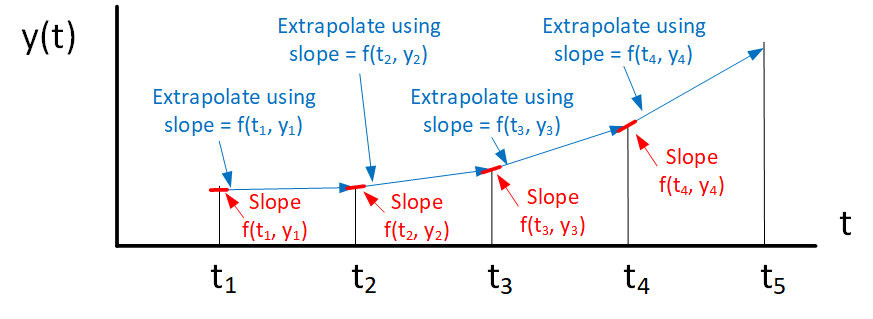
\includegraphics[width=0.8\columnwidth]{ForwardEuler.png}
	\caption{The forward Euler algorithm.  At each time step the algorithm computes the slope of $f(t, y)$, then moves forward by step $h$ to find the next value of $y$.  The slope to use is the slope of the curve at the beginning of the interval.  This figure shows a problem with this algorithm:  the actual solution may curve away from the computed solution since forward Euler uses the old slope at $t_n$ to compute the step, and that slope may not point the method to the correct $y_{n+1}$ at time $t_{n+1}$.}
	\label{fig:ForwardEuler}
\end{figure}
Here are some things to notice about forward Euler:
\begin{itemize}
	\item Refering to \cref{fig:ForwardEuler}, you can see we compute the solution relies on computing the slope of $y$ using $f(t,y)$ (i.e. the derivative) at each point $t_n$, then using the slope to extrapolate $y$ forward one step.  In the figure the thick blue line denotes the slope at each $t_n$.  Note that the slope used is the slope at the beginning of the step interval -- hence the name "forward" Euler.  You can see how each forward step is determined by the slope of the blue line.
	\item Forward Euler is an instance of a so-called "explicit method".  Explicit means all calculations required to take the step are present on the RHS of \cref{eq:FwdEuler}.
	\item \Cref{fig:ForwardEuler} shows clearly a problem with forward Euler:  The actual solution can curve away from the forward Euler solution, causing an error to build up in the forward Euler solution.  The error is clearly dependent upon the size of $h$:  Larger $h$ will lead to larger error, while smaller $h$ leads to smaller error.  The difficulty with smaller $h$ is that smaller step sizes will require more steps -- and longer computation time -- to reach the same end time, $t_{end}$.
\end{itemize}

Besides understanding the math behind the method, there are important implementation features to notice.  The code implementing forward Euler is broken into three parts:  
\begin{enumerate}
\item A top level main program called "test forward euler".  This is the program run by the user.  It sets the model parameters used and invokes the solver itself.  It then makes plots of the result.
\item The solver implementation called "forward euler".  This function is written in a generic way, so it does not set any details of either the parameters of the particular ODE under consideration, nor algorithm features like the step size.  The goal is to have a generic solver which may be used on any ODE without modification.
\item An implementation of the ODE equations contained in a file called "f".  This corresponds to the function $f(t_n, y_n)$ in \cref{eq:FwdEuler}.  Model parameters are passed directly from the top level to "f" as global variables.
\end{enumerate}
A block diagram showing this architecture is presented in \cref{fig:ForwardEulerArch}.  
\begin{figure}[tbh]
	\centering
	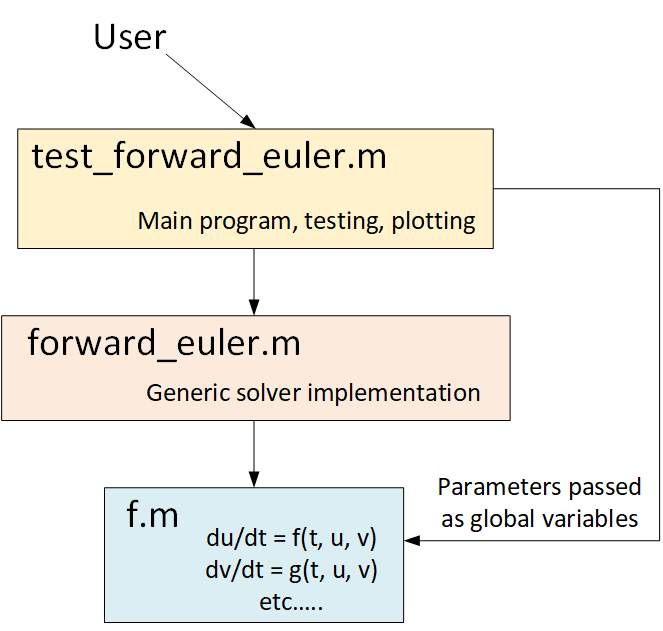
\includegraphics[width=0.5\columnwidth]{ForwardEulerArch.png}
	\caption{The three-layer architecture used in the example Matlab programs implementing forward Euler.  The user runs the main program called "test forward euler".  This in turn calls the solver "forward euler", which in turn calls the function "f" which contains the actual ODE.  A similar design pattern is used for almost all solvers presented in this booklet.}
	\label{fig:ForwardEulerArch}
\end{figure}
The architecture in \cref{fig:ForwardEulerArch} is a simple "software pattern", meaning that it is a good way to partition the code into different pieces, each of which perform a specific function.  Almost all ODE solver examples I present in this booklet are architected using this three-layer pattern.  Real-world ODE solvers like Sundials or DifferentialEquations.jl are also frequently partitioned into different pieces, although their architectures are generally more complicated and have more pieces.  The additional pieces might handle e.g initialization of the solver, management of memory, error handling, sensitivity analysis, and so on.  The point is that it is helpful to partition your program into different pieces which handle logically distinct functions.  Indeed, this is one of the most important things you learn to do when becoming a software engineer.

\section{Example: the exponential growth ODE}
\label{sect:ForwardEulerExponential}
As a first example of our simple solver, we'll apply forward Euler to integrating the exponential growth ODE,
\begin{equation}
\label{eq:ForwardEulerExponential}
\frac{d y}{d t} = \alpha y
\end{equation}
We already know the solution to this equation -- it is $y(t) = y(0) e^{\alpha t}$.  For $\alpha < 0$ the solution decays to zero for $t \rightarrow \infty$, while for $\alpha > 0$ the solution escapes to infinity for $t \rightarrow \infty$.

Now use the prescription to discretize the equation for forward Euler and get
\begin{equation}
y_{n_+1} = y_n + h\alpha y_n
\end{equation}
The result computed using forward Euler is shown in \cref{fig:ForwardEulerExponential} for varying values of $\alpha$.  
\begin{figure}[tbh]
	\centering
	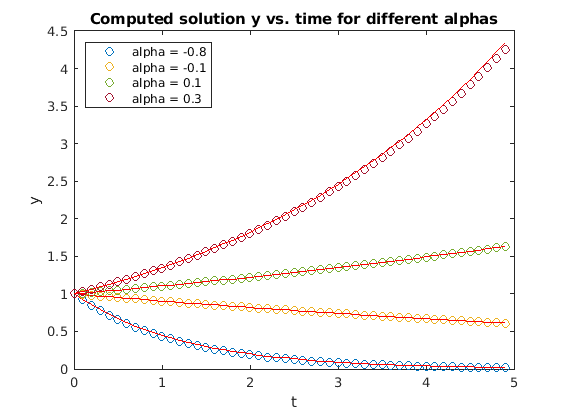
\includegraphics[width=0.7\columnwidth]{ForwardEulerExponential.png}
	\caption{The solution to \cref{eq:ForwardEulerExponential} computed using the forward Euler algorithm for different values of $\alpha$.  The computed function $y_n$ is plotted using open circles and the analytic solution is plotted using red lines.  The stepsize used was $h=0.1$.  Note that the computed and analytic solutions don't exactly match, particularly the case where $\alpha = 0.3$.}
	\label{fig:ForwardEulerExponential}
\end{figure}
The figure shows the computed solution doesn't exactly track the analytic solution.  What is wrong?  The answer has to do with the errors incurred by using the forward difference formula to approximate the derivative.  Recall that the forward difference expression \cref{eq:ForwardDiffApprox1} is only true in the limit where the stepsize goes to zero, $h \rightarrow 0$.  For non-zero $h$, the forward difference approximation is inaccurate, and per the derivation presented in \cref{sect:ForwardDiff} the magnitude of the error scales as $O(h)$.  We can quantify this by examining the RMS error of the computed solution.  The RMS error is computed by comparing the root-mean-square difference between the computed and the analytic solution as follows:
\begin{equation}
\label{eq:RMSErr}
e = \sqrt{\frac{1}{N} \sum_{i=1}^{N} \left( y_t(i) - y_c(i) \right)^2 }
\end{equation}
Here, $y_t$ is the "mathematically true" (analytic) solution, $y_c$ is the solution computed using forward Euler, $N$ is the number of sample points in the solution, and $e$ is the RMS error.  This is also called the "global error" in some textbooks.  We expect that the RMS error will increase with increasing $h$ -- larger stepsizes accumulate larger errors.  The question is, how does the error behave with $h$?  A plot of RMS error vs. $h$ is shown in \cref{fig:ForwardEulerExponentialErr}.  

On the log-log plot the RMS error increases with $h$ by following a straight line.  A useful feature of log-log plots is that it clearly reveals power-law relationships.  Specifically, if a function obeys a power-law $y \sim x^p$ then the slope of the $y$ vs. $x$ line on a log-log plot is the power $p$.  This can be understood by taking the log of both sides of the power-law (which is what plotting on a log-log scale does) and noting that $p$ becomes the slope of the line.
\begin{figure}[tbh]
	\centering
	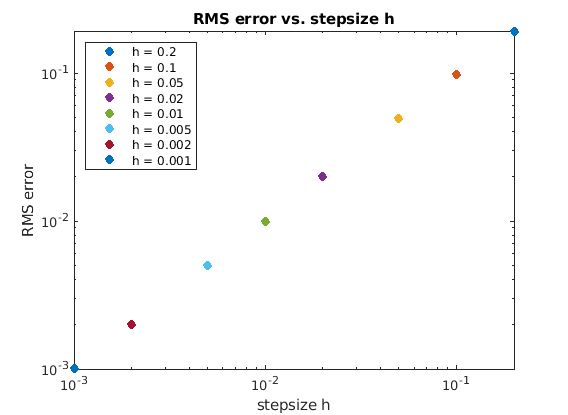
\includegraphics[width=0.7\columnwidth]{ForwardEulerExponentialErr.png}
	\caption{The error incurred by the forward Euler method vs. stepsize $h$ plotted on a log-log scale.  Note that the slope of the error points is one.  This implies the error $e \sim O(h)$.}
	\label{fig:ForwardEulerExponentialErr}
\end{figure}
The slope of the line in \cref{fig:ForwardEulerExponentialErr} is exactly 1 -- This means the RMS error incurred by the forward Euler method is proportional to the stepsize $h$ -- that is, error $e \sim O(h)$.   This scaling relationship was derived in \cref{sect:ForwardDiff} when the forward difference expression was derived from the Taylor series -- terms of $O(h)$ and above were discarded to get the forward difference expression, which means that using the approximation carries an $O(h)$ error penalty.


\section{Detour: Local truncation error vs. global solution error}
Back in \cref{sect:ForwardDiff} I showed how the approximations to the derivative were derived from the Taylor series.  I also mentioned that by dropping higher-order terms, we were implicitly accepting that our computed solutions could only be approximations to the "mathematically true" solution.  That is, the computed solution carried an error, and the major cause of error was due to truncating the Taylor series.  This error is sometimes called the "local truncation error" or "LTE" in the ODE literature.  We generally characterize the LTE in terms of the stepsize scaling $O(h^p)$.  Generally, the error order $p$ is the same as the first truncated term in the Taylor series.  That is, if the first truncated term is $h$ then the LTE scales as $O(h)$.

Now in the previous section we introduced the RMS error \cref{eq:RMSErr}.  Since the RMS error is a sum over the entire solution, it is a global error -- it adds up contributions from all errors present in the entire solution.  (It is normalized by $N$, but nonetheless is sensitive to all errors.)  Therefore, this error is sometimes called the "global error" or GE in the ODE literature.  Again, the GE is characterized by how it scales with $h$.  All error analyses shown in this booklet are global errors computed using the formula  \cref{eq:RMSErr} and are expressed as scaling plots similar to that shown in \cref{fig:ForwardEulerExponentialErr}.

The LTE and the GE are conceptually distinct quantities.  Therefore, you might ask "what is the relationship between the two?"  That is, do they measure the same thing?  The answer is "yes".  Although I won't do it here, it can be proven that the LTE and the GE obey the same scaling relationship for any given method.  That is, if the LTE scales as $O(h^p)$, then the GE also scales as $O(h^p)$.  Accordingly, although I speak loosely about "the error" without quantifying exactly what I mean, the equivalence of the LTE and the GE are sufficient to guarantee the term "the error" refers to something which may be quantified, and is a meaningful metric with which to measure the different ODE solvers presented in this booklet.



\section{Example: a driven system}
Now back to solving ODEs.  A slightly more complicated ODE is this linear ODE with a driving term.  
\begin{equation}
\label{eq:ForwardEulerDriven}
\frac{d y}{d t} = A \sin(\omega t) - \alpha y
\end{equation}
Since the equation is linear, the general solution is the sum of two pieces:  a homogeneous term and an inhomogeneous term (sometimes called the "particular solution").  We'll consider the case of positive $\alpha$.  That is, for $t \rightarrow \infty$ the homogeneous solution will decay away as $e^{-\alpha t}$ so the long-term behavior of the system is determined by the forcing term $A \sin(\omega t)$.   
The analytic solution to the equation is may be found after some algebra,
\begin{equation}
\label{eq:AnalyticDriven}
y(t) = C e^{-\alpha t} + B \cos(\omega t + \phi)
\end{equation}
We adjust the constants $B$, $C$, and $\phi$ to match the initial conditions as well as ensure the particular solution obeys 
\cref{eq:ForwardEulerDriven} for $t \rightarrow \infty$.  To make the plot shown below in \cref{fig:ForwardEulerDriven1} we choose $y(0) = 1$.  With this initial condition, an exercise in easy algebra will show the fitting constants are
\begin{align}
\nonumber
\phi &= \arctan \left( \frac{\alpha}{\omega} \right) \\
\nonumber
B &= \frac{-A}{\omega \cos(\phi) + \alpha \sin(\phi)} \\
\nonumber
C &= 1 - B \cos(\phi)
\end{align}

Discretized for forward Euler, the iteration is
\begin{equation}
y_{n_+1} = y_n + h(A \sin(\omega t_n) - \alpha y_n)
\end{equation}
\Cref{fig:ForwardEulerDriven1} shows the computed solution to \cref{eq:ForwardEulerDriven} for 15 seconds assuming $A = 1.5$, $\omega = 5$ and $\alpha = 0.5$.  The solution clearly shows an initial transient which decays away, leaving a solution which behaves like a sine wave as $t \rightarrow \infty$.
\begin{figure}[tbh]
	\centering
	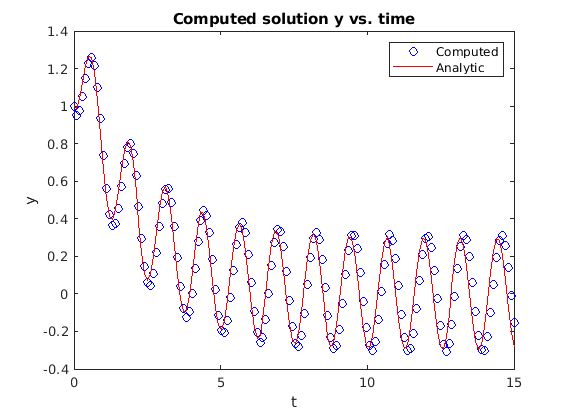
\includegraphics[width=0.7\columnwidth]{ForwardEulerDriven.png}
	\caption{The solution to \cref{eq:ForwardEulerDriven} computed using the forward Euler algorithm.  The computed function $y_n$ is plotted by the blue circles and the analytic solution is plotted using red lines.  Although the two solutions are close, they don't exactly match, and the forward Euler solution seems to diverge from the analytic solution with increasing $t$.}
	\label{fig:ForwardEulerDriven1}
\end{figure}

\section{Example: the logistic equation}
Here is an example of a nonlinear ODE: the logistic equation.  This ODE can be regarded as a very simple model of population dynamics.  Here's the ODE:
\begin{equation}
\label{eq:ForwardEulerLogistic}
\frac{d y}{d t} = \left( 1 - \frac{y}{Y_m} \right) y
\end{equation}
If you think of $y$ as the population of some animal species, when $y \ll Y_m$, then the population can grow exponentially.  But as the population $y \rightarrow Y_m$, the growth rate of the population saturates.  Think of rabbits living in a carrot field -- when there are very few rabbits (and no preditors) then the rabbits have lots of carrots to eat and they may reproduce freely, leading to exponential growth.  However, if too many rabbits live in the field, then they eat most of the carrots and can't reproduce freely anymore since food is scarce.  Consequently, the rabbit population tends towards a fixed limit given by $y = Y_m$.

This equation has the following analytic solution:
\begin{equation}
\label{eq:AnalyticLogistic}
y(t) = \frac{y_0 e^t}{ \left( 1 + \frac{y_0}{Y_m} e^t \right) }
\end{equation}
where $y_0$ is used to match the initial condition.  Inspection shows $y_0 = y(t=0)$.  Also note that when $y = Y_m$ the growth rate (derivative) goes to zero, consistent with the intuition that the rabbit population should saturate when the rabbits eat most of the carrots.  Just enough carrots remain to carry the rabbit population, but the population can't grow any more.

Discretized for forward Euler, the iteration to implement for the logistic equation is 
\begin{equation}
y_{n_+1} = y_n + h \left( 1 - \frac{y_n}{Y_m} \right) y_n
\end{equation}
This iteration was implemented in Matlab and then run for three different values of $Y_m$. The results are shown in \cref{fig:ForwardEulerLogistic}.
\begin{figure}[tbh]
	\centering
	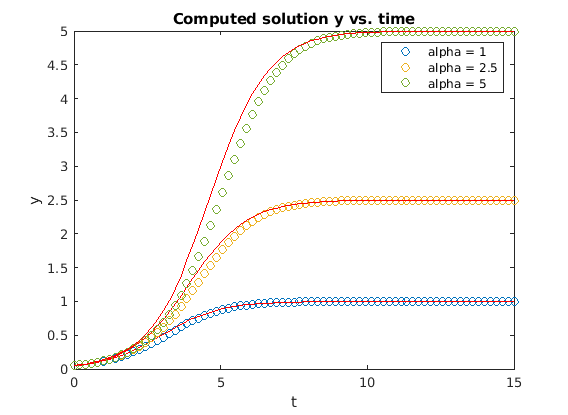
\includegraphics[width=0.7\columnwidth]{ForwardEulerLogistic.png}
	\caption{The solution to \cref{eq:ForwardEulerLogistic} computed using the forward Euler algorithm for three different $Y_m$ values.  The computed function $y_n$ is plotted using open circles and the analytic solution is plotted using red lines.  Note that the computed solution lags (is behind) the analytic solution -- forward Euler's solution carries an error.  One can imagine the rabbit population starting from a low base and growing until it hits a saturation point.  The saturation point is determined by the value of $Y_m$.}
	\label{fig:ForwardEulerLogistic}
\end{figure}
Forward Euler reproduces the saturation behavior of the logistic equation quite well -- after around $t = 10$ the forward Euler solution matches the analytic solution.  However, forward Euler does a worse job reproducing the period of exponential growth around $t = 5$ -- forward Euler lags the analytic solution.  This behavior is similar to that observed in the exponential growth ODE shown in \cref{fig:ForwardEulerExponential}.


\section{Extending Forward Euler to higher order}  
\label{sect:HigherOrderForwardEuler}
So far, we have dealt with scalar, first-order ODEs like that shown in Equation \cref{eq:FirstOrderODE}.  Many ODEs encountered in practice are higher order.  For example, consider the most famous second order ODE of all: Newton's second law:  $F = ma$.  It says that imposing a force on a body will cause it to accelerate in the direction of the applied force.  Since acceleration is the second derivative of the body's position, $a = d^2 y/ d t^2$, this implies we can write Newton's second law as an ODE:
\begin{equation}
\label{eq:2ndOrderODE}
\frac{d^2 y}{d t^2} = F(t, y', y) 
\end{equation}
Given the importance of Newton's law, we want to be able to solve ODEs like \cref{eq:2ndOrderODE} numerically.  How to extend the forward Euler method to second (and higher) order ODEs?

The way to solve \cref{eq:2ndOrderODE} numerically is to rearrange it to become two first order ODEs as follows:
\begin{enumerate}
	\item Define two variables, $y_1 = dy/dt$ and $y_2 = y$.
	\item Now note that \cref{eq:2ndOrderODE} may be written as
	\begin{equation}
	\nonumber
	\frac{d y_1}{d t} = \frac{d^2 y}{d t^2} = F(t, y', y)
	\end{equation}
	\item Next, by definition we have
	\begin{equation}
	\nonumber
	\frac{d y_2}{d t} = \frac{d y}{d t} = y_1
	\end{equation}
	\item Therefore, we have broken  \cref{eq:2ndOrderODE} up into two coupled, first-order ODEs,
	\begin{align}
	\nonumber
	\frac{d y_1}{d t} &= F(t, y_1, y_2) \\
	\nonumber
	\frac{d y_2}{d t} &= y_1
	\end{align}
	\item This system of two first order ODEs may be solved using forward Euler using the same methods as in \cref{sect:ForwardEulerMethod}.
\end{enumerate}
This technique of breaking a second order ODE into two first order ODEs may be easily generalized.  As a rule, if you start with an $n$th order ODE you may break it down into $n$ first order ODEs.  Then the system of first order ODEs may be solved using forward Euler or any of the more advanced methods we will encounter later.

It's not enough to simply specify the equations to solve.  We also need to specify intial conditions (ICs) for this system -- one IC for each equation.  In general, an $n$th order ODE will be accompanied by $n$ initial conditions, usually one for the function $y(t=0)$, one for the first derivative $y'(t=0)$, one for the second derivative $y''(t=0)$, and so on.  Therefore, a second order ODE such as \cref{eq:2ndOrderODE} will require two ICs.  Using the definitions of $y_1$ and $y_2$ above, it's easy to map the ICs for the second order equation onto the ICs for the system as
\begin{align}
\nonumber
y_1(0) &= y'(0) \\
\nonumber
y_2(0) &= y(0)
\end{align}


\section{Example: the simple harmonic oscillator}
\label{sect:SHO}
To make these ideas concrete we will examine the so-called simple harmonic oscillator (SHO).  This is a simple model of oscillatory motion beloved by physicists, and encountered in many real-world applications.  One situation modeled by the SHO is a mass sliding on a (frictionless) floor, and tethered to a wall by a spring.  See \cref{fig:SlidingSHO}.  The force impressed by the spring on the mass is modeled using Hooke's law, which says the spring tries to restore the mass to an equilibrium position with a force varying linearly with position.  Taking $y$ as the position of the mass, Hooke's law says $F = -k (y-y_r)$, where $k$ is a constant measuring the stiffness of the spring, and $y_r$ is the rest position of the mass.  From now on out we will set $y_r = 0$ since it is a constant and doesn't affect the math we want to explore.
\begin{figure}[tbh]
	\centering
	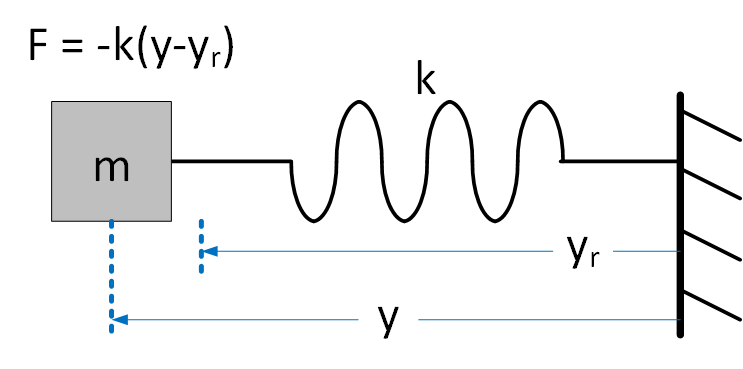
\includegraphics[width=0.5\columnwidth]{SlidingSHO.png}
	\caption{The simple harmonic oscillator (SHO).  The mass $m$ slides frictionlessly on the floor.  It is attached to a wall through a spring.  The spring constant (measure of spring stiffness) is $k$.  When the mass is displaced from its rest position $y_r$ the spring tends to push or pull the mass back to the rest position.  However, the mass overshoots the rest position due to Newton's second law.  Therefore, the spring will execute a sinusoidal oscillation around $y_r$, and if the system is lossless the oscillation will never stop.  The oscillatory motion is governed by \cref{eq:SHO}, which is known as the simple harmonic oscillator equation.}
	\label{fig:SlidingSHO}
\end{figure}

Combining Hooke's law and Newton's second law, we can write down a second order ODE describing the motion of the mass under the influence of the spring,
\begin{equation}
\label{eq:SHO}
\frac{d^2 y}{d t^2} = -\frac{k}{m} y
\end{equation}
You probably already know the solution(s) to this equation.  They are sines and cosines,
\begin{equation}
y(t) = A \cos(\omega t) + B \sin(\omega t)
\end{equation}
where we have defined $\omega = \sqrt{k/m}$ for convenience. $\omega$ is generally referred to as the oscillation frequency.  The coefficients $A$ and $B$ are determined by the initial conditions.

How to solve \cref{eq:SHO} numerically?  We'll use our prescription from \cref{sect:HigherOrderForwardEuler} and break \cref{eq:SHO} into two first order ODEs.  We define $u = dy/dt$ and $v = y$.  (I use $u$ and $v$ instead of $y_1$ and $y_2$ for notational convenience in what comes next.) Now we can decompose \cref{eq:SHO} into
\begin{equation}
\label{SHOSystem}
\begin{aligned}
\frac{d u}{d t} &= -\frac{k}{m} v  \\
\frac{d v}{d t} &= u
\end{aligned}
\end{equation}
Now discretize using the forward difference approximation to the first derivative:
\begin{align}
\nonumber
\frac{u_{n+1} - u_{n}}{h} &= -\frac{k}{m} v_n  \\
\nonumber
\frac{v_{n+1} - v_{n}}{h} &= u_n
\end{align}
Next rearrange these equations to place the future on the LHS and the present on the RHS:
\begin{equation}
\begin{aligned}
u_{n+1} &= u_n -h \frac{k}{m} v_n  \\
v_{n+1} &= v_n + h u_n
\end{aligned}
\label{eq:SHOSystem}
\end{equation}
Now we have a pair of equations which we can step forward in time!  We start with known initial conditions $u_0$  and $v_0$ and use the system to compute the next values in time $u_1$  and $v_1$, then use those to get the next values, and so on.

This algorithm is easy to implement using e.g. Matlab.  The results of running a Matlab program implementing the iteration \cref{eq:SHOSystem} are shown in \cref{fig:ForwardEulerSHO}.  Results for two different step sizes ($h = 0.01$ and $h = .001$) are shown for comparison.  The initial conditions $u_0 = 1$ and $v_0 = 0$ were used in both cases.  These ICs correspond to an oscillating mass whose starting position is 1 and whose starting velocity is 0 -- similar to pulling the mass by hand to position 1, holding it there for a moment, then releasing it.  
\begin{figure}[tbh]
	\centering
	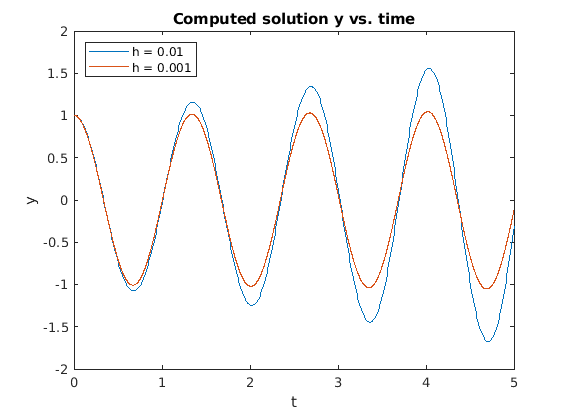
\includegraphics[width=0.7\columnwidth]{ForwardEulerSHO.png}
	\caption{The simple harmonic oscillator (SHO) solved using forward Euler.  Note that the sinusoidal amplitude increases exponentially with time.  This is contrary to the known solution involving pure sins and cosines.  Why does this happen? This effect has to do with the concept of stability discussed later in \cref{sect:stability}.}
	\label{fig:ForwardEulerSHO}
\end{figure}
Things to note in the figure:
\begin{itemize}
	\item Both plots show the mass oscillates back and forth in time.  This is to be expected, since the solutions to \cref{eq:SHO} are sines and cosines.
	\item However, we see that both solutions grow in time.  The $h = 0.01$ solution grows faster than the $h = .001$ one, but close inspection of the plot shows they both grow.  This is unexpected, and is incorrect -- the ODE \cref{eq:SHO} has sin and cos solutions which don't grow.  What is wrong?  The answer to this question involves studying the stability of the forward Euler method.
\end{itemize}

\section{Propagator matrix for SHO}
\label{sect:SHOPropagator}
Before we talk about stability, it is convenient to recast the iteration \cref{eq:SHOSystem} into a different format.
Because \cref{eq:SHO} is linear, we can take the forward Euler system one step further.  Note that the following doesn't work with all ODEs -- only with linear ODEs!  With a little rearranging we can write \cref{eq:SHOSystem} as a matrix-vector system,
\begin{align}
\label{eq:SHOMatVecSystem}
\begin{pmatrix}
u_{n+1} \\
v_{n+1}
\end{pmatrix}
=
\begin{pmatrix}
1 & - h k / m \\
h & 1
\end{pmatrix}
\begin{pmatrix}
u_{n} \\
v_{n}
\end{pmatrix}
\end{align}
or, written in matrix-vector form,
\begin{equation}
\label{eq:SHOMatVecForm}
\nonumber
{y_{n+1}} = {A} {y_n}
\end{equation}
where 
\begin{equation}
\nonumber
{y_n} = 
\begin{pmatrix}
u_{n} \\
v_{n}
\end{pmatrix}
\end{equation}
and ${A}$ is the matrix shown in \cref{eq:SHOMatVecSystem}.   ${A}$ is commonly called the "propagator matrix" since repeated multiplication by ${A}$ propagates (steps) the solution ${y_n}$ forward in time.

Pseudocode implementing the forward Euler algorithm to solve the simple harmonic oscillator is shown in \cref{alg:FwdEulerSHO}.
\begin{algorithm}
	\caption{Forward Euler method for SHO}
	\label{alg:FwdEulerSHO}
	\begin{algorithmic} 
		\STATE {Inputs: initial condition ${y_0} = [u_0, v_0]^T$, end time $t_{end}$.}
		\STATE {Initialize: $t_0=0$, ${y_0}$.} 
		\FOR{$n=0:t_{end}/h$} 
		\STATE ${y_{n+1}} \leftarrow {A} {y_n}$
		\ENDFOR
		\RETURN ${y_n}$.
	\end{algorithmic}
\end{algorithm}
The results of a run using this propagator method are shown in \cref{fig:ForwardEulerSHOPropagator}.  The results are the same as those obtained in \cref{sect:SHO}
\begin{figure}[tbh]
	\centering
	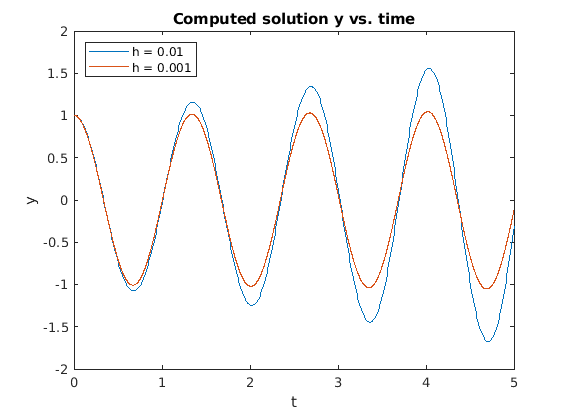
\includegraphics[width=0.7\columnwidth]{ForwardEulerSHOPropagator.png}
	\caption{The simple harmonic oscillator (SHO) integrated using the propagator iteration.  Use of the propagator matrix only works when the ODE under consideration is linear and each step may be turned into a matrix-vector multiplication.}
	\label{fig:ForwardEulerSHOPropagator}
\end{figure}

\section{Stability}
\label{sect:stability}
In deriving the expressions for finite difference approximations we found that the process of discretization produced a difference (error) between the exact (analytical) derivative and the finite difference approximation.  Now we find a second pitfall in numerically solving ODEs:  Growning numerical solutions when we know the exact (analytic) solution should not grow in time.  What is happening?

\subsection{Stability of forward Euler for the exponential growth ODE}
To understand the observed growth consider the exponential growth ODE:
\begin{equation}
\label{eq:SimpleLinearODE}
\frac{dy}{dt} = a y
\end{equation}
Note that this ODE is linear.  We know this equation has an exact, mathematically-true solution $y_t(t) = y_0 e^{a t}$, where we denote the exact, mathematically-true solution as $y_t$.  Now ask the question: What happens if the exact solution is perturbed by some error $e$?  That is, take $y = y_t(t) + e(t)$.  In this case linearity says we can write
\begin{equation}
\nonumber
\frac{dy_t}{dt} + \frac{de}{dt} = a (y_t + e)
\end{equation}
This equation separates into two pieces,
\begin{equation}
\nonumber
\frac{dy_t}{dt} = a y_t
\end{equation}
which is satisfied identically because $y_t$ is the exact solution by definition, and 
\begin{equation}
\nonumber
\frac{de}{dt} = a e
\end{equation}
Which governs the behavior of the error term $e$.  Now discretize this term 
using the forward Euler method to get
\begin{equation}
\label{eq:fwdeulerexpgrowth}
e_{n+1} = e_n + h a e_n = (1 + a h)e_n
\end{equation}
where $e_n$ is the error at step $n$.  Assuming we start with a small perturbation $e_0$ at time $t=0$, and just watch the evolution of this one perturbation in time, we find \cref{eq:fwdeulerexpgrowth} behaves as
\begin{equation}
e_{n} = (1 + a h)^n e_0
\end{equation}
Clearly, the perturbation grows exponentially as $n \rightarrow \infty$ if $\lvert 1 + a h \rvert > 1$ but decays to zero as long as
\begin{equation}
\label{eq:ForwardEulerStabilityCond}
\lvert 1 + a h \rvert < 1
\end{equation}
\Cref{eq:ForwardEulerStabilityCond}  is the forward Euler stability condition for the exponential growth ODE.
A solver applied to an ODE is stable if an initial error or perturbation either maintains the same magnitude or dies out in time.  But if an initial error grows exponentially, then the solver is unstable.  Note that the property of stability depends upon both the solver and the ODE itself -- a solver which is stable for one ODE might be unstable for a different one, and different solvers may be stable or unstable for the same ODE.  

So now the question becomes, when is forward Euler stable for the simple ODE \cref{eq:SimpleLinearODE}?  For forward Euler to make sense, the step $h$ must be a small, positive number.  However, we have placed no constraints on $a$ -- it can be positive, negative, or even complex.  Therefore, to understand when \cref{eq:SimpleLinearODE} is stable it makes sense to plot the region of stability in the complex plane of $a h$.  This is shown in \cref{fig:ForwardEulerStabilityRegion}. The region of stability is the grey circle to the left of the origin.  
Values inside the circle represent $a h$ values which do not blow up -- they are stable because they satisfy the stability condition $\lvert 1 + a h \rvert < 1$.  
\begin{figure}[tbh]
	\centering
	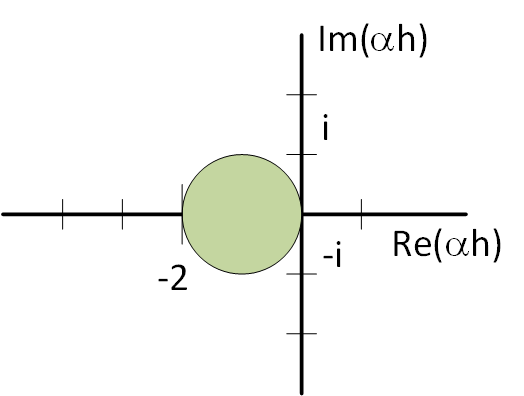
\includegraphics[width=0.5\columnwidth]{ForwardEulerStabilityRegion.png}
	\caption{Forward Euler's stability region for the simple linear ODE \cref{eq:SimpleLinearODE}.  The stability region for this system is a circle of radius 1 in the complex plane centered at $a h = -1$.}
	\label{fig:ForwardEulerStabilityRegion}
\end{figure}


\subsection{Stability of forward Euler for the simple harmonic oscillator}
\label{sect:FwdEulerSHOStability}
Now we consider the stability of forward Euler applied to the simple harmonic oscillator.  Recall the forward Euler iteration for this equation,
\begin{align}
\label{eq:SHOMatVecSystem1}
\begin{pmatrix}
u_{n+1} \\
v_{n+1}
\end{pmatrix}
=
\begin{pmatrix}
1 & -h k / m \\
h & 1
\end{pmatrix}
\begin{pmatrix}
u_{n} \\
v_{n}
\end{pmatrix}
\end{align}
We know the "mathematically-true" solution to the SHO is composed of sines and cosines, or equivalently of complex exponentials, $e^{i \omega t}$.  We'll choose one solution,
\begin{align}
\nonumber
%\label{eq:SHOMatVecSystem1}
\begin{pmatrix}
u_{n} \\
v_{n}
\end{pmatrix}
=
\begin{pmatrix}
e^{i \omega t} \\
i \omega e^{i \omega t}
\end{pmatrix}
\end{align}
and examine its time evolution.  
Instead of considering an additive perturbation, we instead consider tracking errors using a multiplicative "error factor" $e_n$.  That means we assume the solution 
\begin{align}
\label{eq:SHOWithGrowth}
\begin{pmatrix}
u_{n} \\
v_{n}
\end{pmatrix}
=
e_n
\begin{pmatrix}
e^{i \omega t} \\
i \omega e^{i \omega t}
\end{pmatrix}
\end{align}
and insert it into \cref{eq:SHOMatVecSystem1} and see how $e_n$ behaves in time.  Clearly, if $e_n = 1$ for all time, then \cref{eq:SHOWithGrowth} solves \cref{eq:SHOMatVecSystem1} exactly.  But if $e_n \ne 1$ then the forward Euler iteration introduces errors to the solution.

Inserting \cref{eq:SHOWithGrowth} into \cref{eq:SHOMatVecSystem1} we get
\begin{equation}
\nonumber
e_{n+1}
\begin{pmatrix}
e^{i \omega (t+h)} \\
i \omega e^{i \omega (t+h)}
\end{pmatrix}
=
e_n
\begin{pmatrix}
	1 & -\frac{h k}{m} \\
	h & 1
\end{pmatrix}
\begin{pmatrix}
e^{i \omega t} \\
i \omega e^{i \omega t}
\end{pmatrix}
\end{equation}
Now divide out by the common factor $e^{i \omega t}$ and define the so-called "growth factor", $g_n = e_{n+1}/e_n$ to get
\begin{equation}
\nonumber
g_n e^{i \omega h}
\begin{pmatrix}
1 \\
i \omega 
\end{pmatrix}
=
\begin{pmatrix}
1 & -\frac{h k}{m} \\
h & 1
\end{pmatrix}
\begin{pmatrix}
1 \\
i \omega 
\end{pmatrix}
\end{equation}
Now we see that this expression has the form of an eigenvalue problem, $ \lambda {x} = {A} {x}$, where the scalar $g_n e^{i \omega h}$ plays the role of the eigenvalue.  We can solve for $g_n e^{i \omega h}$ the usual way by subtracting the LHS from the RHS,
\begin{equation}
\nonumber
\begin{pmatrix}
	1 - g_n e^{i \omega h} & -\frac{h k}{m} \\
	h & 1 - g_n e^{i \omega h} 
\end{pmatrix}
\begin{pmatrix}
	1 \\
	i \omega 
\end{pmatrix}
= 0
\end{equation}
and observing that for this to hold, we need values of $g_n e^{i \omega h}$ which make the matrix singular.  Therefore, we require
\begin{equation}
\nonumber
\begin{vmatrix}
1 - g_n e^{i \omega h} & -\frac{h k}{m} \\
h & 1 - g_n e^{i \omega h} 
\end{vmatrix}
= 0
\end{equation}
or
\begin{equation}
\nonumber
(1 - g_n e^{i \omega h})^2  + h^2 \frac{k}{m} 
= 0
\end{equation}
Next, again recall the definition of the "natural frequency" of the SHO, $\omega_0^2 = k/m$.  Then rearrange to solve for $g_n$ and get
\begin{equation}
\nonumber
(1 - g_n e^{i \omega h})^2 = -h^2 \omega_0^2 
\end{equation}
or
\begin{equation}
\nonumber
g_n e^{i \omega h} = 1 \pm i h \omega_0
\end{equation}
Now we ask, under which conditions does the error factor $e_n$ remain constant, or at least not grow or shrink?  $e_n$ remains constant as long as $|g_n| = 1$.  That is, we require
\begin{equation}
\label{eq:fwdEulerGrowthFactor}
|g_n| = \left| 1 \pm i h \omega_0 \right|
\end{equation}
However, this clearly never happens -- the RHS of \cref{eq:fwdEulerGrowthFactor} is always greater than one.  This is evident by inspecting the RHS in the complex plane as shown in \cref{fig:ForwardEulerSHOComplexPlane}
\begin{figure}[tbh]
	\centering
	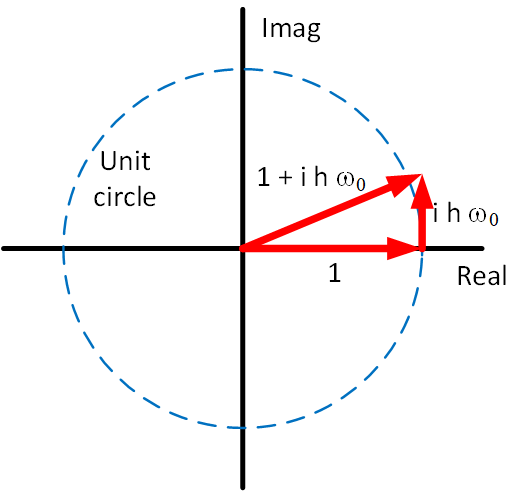
\includegraphics[width=0.5\columnwidth]{ForwardEulerSHOComplexPlane.png}
	\caption{The RHS of \cref{eq:fwdEulerGrowthFactor}.  The real part is always 1, while the imaginary part can take any value.  However, as long as the imaginary part is not identically zero, then the magnitude of $1 \pm i h \omega_0$ is always greater than 1.  Therefore, the error factor $e_n$ will always grow, and the SHO is always unstable for any non-zero stepsize $h$.}
	\label{fig:ForwardEulerSHOComplexPlane}
\end{figure}
Therefore, the solution computed by forward Euler always grows.  For increasingly small step size $h$ the growth factor tends to 1, but never reaches 1 until $h$ is exactly zero -- a situation which makes the forward Euler method useless since you can't step forward in time if $h = 0$.  This means the forward Euler method is never useful for solving the simple harmonic oscillator problem -- we need to find better methods.

\section{Chapter summary}
Here are the important points made in this chapter:
\begin{itemize}
\item The forward Euler method is derived from the simple forward difference expression for the derivative, $y' = (y_{n+1} - y_n)/h$.
\item The forward Euler method is an iterative method which starts at an initial point and walks the solution forward using the iteration $y_{n+1} = y_n + h f(t_n, y_n)$.
\item Since the future is computed directly using values of $t_n$ and $y_n$ at the present, forward Euler is an explicit method.
\item The forward Euler method is defined for 1st order ODEs.  It works for both one- and many-variable ODEs.  To solve an Nth order ODE one breaks the ODE into N first order ODEs.
\item The RMS error expected when using the forward Euler method scales as $e \sim O(h)$.
\item Solver stability is not guaranteed for all step sizes $h$.  The stability criterion depends upon the exact ODE under consideration, but in general smaller step sizes are required for stability when using explicit methods.
\end{itemize}

%%%%%%%%%%%%%%%%%%%%%%%%%%%%%%%%%%%%%%%%%%%%%%%%%%%%%%%%%%%%%%%%%%%%%%%%%%%%%%%%%%%%%%%%%%%%%%%%%%%%%%%%%%%%%%%%%%%%%%%%%
%%%%%%%%%%%%%%%%%%%%%%%%%%%%%%%%%%%%%%%%%%%%%%%%%%%%%%%%%%%%%%%%%%%%%%%%%%%%%%%%%%%%%%%%%%%%%%%%%%%%%%%%
\chapter{Backward Euler method}
\section{Backward Euler algorithm}
The next ODE solver is called the "backward Euler method" for reasons which will quickly become obvious.  Start with the first order ODE,
\begin{equation}
\label{eq:FirstOrderODE1}
\frac{d y}{d t} = f(t, y) 
\end{equation}
then recall the backward difference approximation,
\begin{equation}
\nonumber
\frac{d y}{d t} \approx \frac{y_n - y_{n-1}}{h}
\end{equation}
We can use this in \cref{eq:FirstOrderODE1} to get
\begin{equation}
\label{eq:BkwdDiff2}
\frac{y_n - y_{n-1}}{h} = f(t_n, y_n) 
\end{equation}
Since we're using backward differencing to derive \cref{eq:BkwdDiff2}, this is the "backward Euler method".   Now shift this forward in time by one step (i.e. replace $n$ by $n+1$ everywhere).  This shift creates a valid equation since \cref{eq:BkwdDiff2} is valid for all $n$.  Upon shifting we get
\begin{equation}
\nonumber
\frac{y_{n+1} - y_{n}}{h} = f(t_{n+1}, y_{n+1}) 
\end{equation}
Now move the future to the LHS and the present to the RHS to get
\begin{equation}
\label{eq:BackwardEulerMethod}
y_{n+1} - h f(t_{n+1}, y_{n+1}) = y_{n}
\end{equation}
Now you might rightly ask, what good does this expression do?  In order to compute the unknown $y_{n+1}$, you need to already know $y_{n+1}$ to use it on the LHS.  But how can you use $y_{n+1}$ if it's the unknown you are solving for?

The answer is that you can turn \cref{eq:BackwardEulerMethod} into a rootfinding problem.  Subtract the known value $y_n$ from both sides of \cref{eq:BackwardEulerMethod}.  Then consider the expression on the LHS to be a function of $y_{n+1}$.  We have
\begin{equation}
\label{eq:BackwardEulerRootfinding}
g(y_{n+1}) =
y_{n+1} - h f(t_{n+1}, y_{n+1}) - y_{n}
= 0
\end{equation}
Therefore, finding $y_{n+1}$ involves finding the root of $g(y_{n+1})$.  In general, $g(y_{n+1})$ can be a nasty, non-linear function of $y_{n+1}$, but such problems are easily handed using numerical methods -- Newton's method immediately springs to mind.  We won't cover rootfinding in this class, but many methods are presented in the standard texts on numerical analysis.

Assuming you can use a rootfinding method to solve \cref{eq:BackwardEulerRootfinding}, you have a time-stepping method:  Start with the initial condition $y_0$, insert it into \cref{eq:BackwardEulerRootfinding}, then use rootfinding to compute $y_1$.  Then using $y_1$ use \cref{eq:BackwardEulerRootfinding} and rootfinding to find $y_2$, and so on.  This is the backward Euler method. 

Pseudocode implementing the backward Euler algorithm to solve the simple harmonic oscillator is shown in \cref{alg:BackwardEulerAlgo}.
\begin{algorithm}
	\caption{Backward Euler method}
	% Must put label after caption for cref to work.
	\label{alg:BackwardEulerAlgo}
	\begin{algorithmic} 
		\STATE {Inputs: initial condition $y_0$, end time $t_{end}$.}
		\STATE {Initialize: $t_0=0$, $y_0$.} 
		\FOR{$n=0:t_{end}/h$} 
		\STATE Form equation for LHS with $y_{n+1}$ as unknown variable, $g(y_{n+1}) = y_{n+1} - h f(t_{n+1}, y_{n+1}) - y_{n}$
		\STATE Solve rootfinding problem $g(y_{n+1}) = 0$ to find $y_{n+1}$.
		\ENDFOR
		\RETURN $y$ vector.
	\end{algorithmic}
\end{algorithm}
A graphical depiction of the algorithm is shown in \cref{fig:BackwardEuler}.
\begin{figure}[tbh]
	\centering
	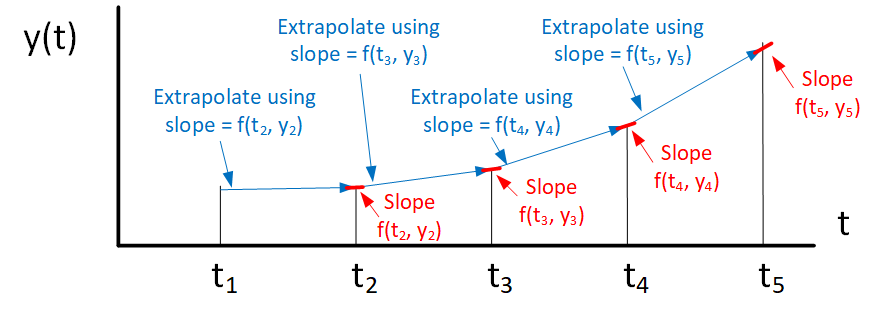
\includegraphics[width=0.8\columnwidth]{BackwardEuler.png}
	\caption{The backward Euler algorithm.  At each time step the algorithm uses rootfinding to get the slope of $y$, then moves forward by step $h$.  The slope used is that at the end of the interval.}
	\label{fig:BackwardEuler}
\end{figure}
Here are some things to note about backward Euler:
\begin{itemize}
	\item Note that the slope used is the slope at the end of the step interval -- hence the name "backward" Euler.  You can see how each step is determined by the slope of the blue line.
	\item The step is not directly calculable from the RHS of \cref{eq:BackwardEulerMethod}.  Rather, rootfinding is required to get the value of $y_{n+1}$ at each step.  Therefore, backward Euler is called an "implicit method".
\end{itemize}


\section{Example: exponential growth ODE}
\label{sect:BkwdEulerExponentialGrowthODE}
As an example of backward Euler we again consider the exponential growth ODE,
\begin{equation}
\label{eq:ExpGrowthODE}
\frac{d y}{d t} = \alpha y
\end{equation}
Discretize using the backward difference approximation to get
\begin{equation}
\nonumber
\frac{y_{n+1} - y_n}{h} = \alpha y_{n+1}
\end{equation}
Move the future to the LHS and the present to the RHS to get
\begin{equation}
\nonumber
y_{n+1} - h \alpha y_{n+1} = y_n
\end{equation}
Since this is a linear equation, deriving the time-stepping method is easy -- no rootfinding required.  We obtain
\begin{equation}
\label{eq:BackwardEulerIterationLinearEq}
y_{n+1}= \frac{y_n}{1  - h \alpha }
\end{equation}
A plot of the solution found via backward Euler when $h = 0.1$ is shown in \cref{fig:BackwardEulerExponential}.  Something is wrong!  The plots do not look like those shown in \cref{fig:ForwardEulerExponential}, nor do they match the analytic result.  What happened?
\begin{figure}[tbh]
	\centering
	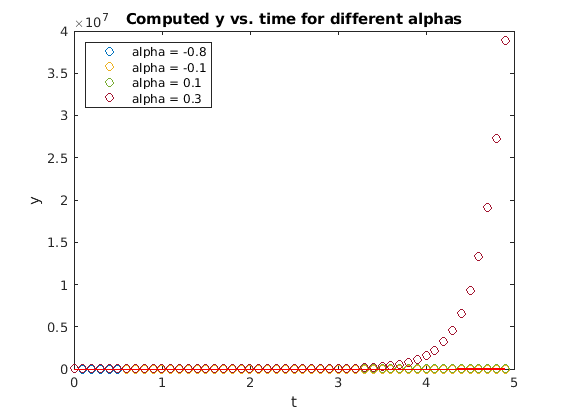
\includegraphics[width=0.5\columnwidth]{BackwardEulerExponential.png}
	\caption{Backward Euler solution of the exponential growth ODE for $h = 0.1$.  Something is obviously wrong!}
	\label{fig:BackwardEulerExponential}
\end{figure}
The biggest hint is the y-axis scale -- it says one of the curves increases to around 4e7 -- a gigantic number.  This is a clear signal backward Euler is unstable for this system.  Stability is therefore the subject of the next subsection.


\subsection{Stability of backward Euler for the exponential growth ODE}
Now we derive the domain of stability for the backward Euler method.  We again consider the exponential growth equation \cref{eq:ExpGrowthODE} first presented in \cref{sect:ForwardEulerExponential}.  Following an argument similar to that presented in \cref{sect:ForwardEulerExponential} we may derive the following expression for the growth of an initial perturbation:
\begin{equation}
\nonumber
e_{n+1} = \frac{e_n}{1 + a h}
\end{equation}
Note the similarity of this expression to \cref{eq:BackwardEulerIterationLinearEq} in the last section.  The similarity holds because of the linearity of \cref{eq:ExpGrowthODE}.  
Assuming the start perturbation at time $t=0$ is $e_0$, the error grows as
\begin{equation}
e_n = \left( \frac{1}{1+a h} \right)^n e_0
\end{equation}
For the error to remain bounded, we require
\begin{equation}
\nonumber
\left| \frac{1}{1+a h} \right| \le 1
\end{equation}
or
\begin{equation}
\left| 1+a h \right| \ge 1
\end{equation}
A plot of the region in the complex plan where the error is bounded (i.e. where backward Euler is stable for this ODE) is shown in \cref{fig:BackwardEulerStabilityRegion}.  Note that this stability region is the complement of that obtained for forward Euler -- backward Euler is stable for large relative step values (large $a h$) while forward Euler is only stable for small steps.  Compare the stability regions shown here to that shown in \cref{fig:ForwardEulerStabilityRegion}.
\begin{figure}[tbh]
	\centering
	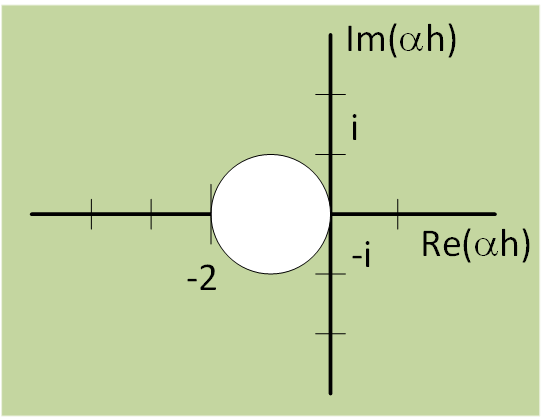
\includegraphics[width=0.5\columnwidth]{BackwardEulerStabilityRegion.png}
	\caption{Backward Euler's stability region for the exponential growth ODE \cref{eq:ExpGrowthODE}.  The stability region includes the entire complex plane with the exception of the circle of radius 1 in the complex plane centered at $a h = -1$.}
	\label{fig:BackwardEulerStabilityRegion}
\end{figure}
Thinking back to the results obtained in \cref{sect:BkwdEulerExponentialGrowthODE} for the exponential growth ODE, recall we set $h = 0.1$ and simulated a number of different $\alpha$ values.  For each $\alpha$ value we have
\begin{itemize}
	\item $\alpha = -0.8$, $\alpha h = -0.08$.  This lies inside the unstable circle in \cref{fig:BackwardEulerStabilityRegion}.  Unstable!
	\item $\alpha = -0.1$, $\alpha h = -0.01$.  This lies inside the unstable circle in \cref{fig:BackwardEulerStabilityRegion}.  Unstable!
	\item $\alpha = 0.1$, $\alpha h = 0.01$.  This lies outside the unstable circle in \cref{fig:BackwardEulerStabilityRegion}.  Stable.
	\item $\alpha = 0.3$, $\alpha h = 0.03$.  This lies outside the unstable circle in \cref{fig:BackwardEulerStabilityRegion}.  Stable.
\end{itemize}
Therefore, the bad results shown in \cref{fig:BackwardEulerExponential} are due to the fact that two of the $\alpha h$ values are in the unstable area.


\section{Example: the logistic equation}
Recall the logistic equation, \cref{eq:ForwardEulerLogistic}.  
We discretize for backward Euler by putting the future on the LHS and the present on the RHS.  In this case the iteration is 
\begin{equation}
\nonumber
y_{n+1} - h \left( 1 - \frac{y_{n+1}}{Y_m} \right)y_{n+1} = y_n
\end{equation}
This is a nonlinear equation, so a rootfinder is required to implement the backward Euler iteration.  That is, upon every iteration the following equation is solved to find the value of $y_{n+1}$
\begin{equation}
\nonumber
g(y_{n+1}) = y_{n+1} - h \left( 1 - \frac{y_{n+1}}{Y_m} \right)y_{n+1} - y_n = 0
\end{equation}
The parameters $h$ and $Y_m$ are inputs to the problem and are therefore known quantities.  Also, since at each step we start at $t_n$, the value $y_n$ is also known.  That means $y_{n+1}$ is the only unknown and it is the quantity we solve for.  A solver like Newton's method, or the Matlab built-in function "fsolve()" are perfectly suited to compute the required value of $y_{n+1}$.

This iteration was implemented in Matlab and then run for three different values of $Y_m$. The results are shown in \cref{fig:BackwardEulerLogistic}.  The computed solution leads the analytic solution.  Compare this to \cref{fig:ForwardEulerLogistic}, where the computed solution trails the analytic solution.
\begin{figure}[tbh]
	\centering
	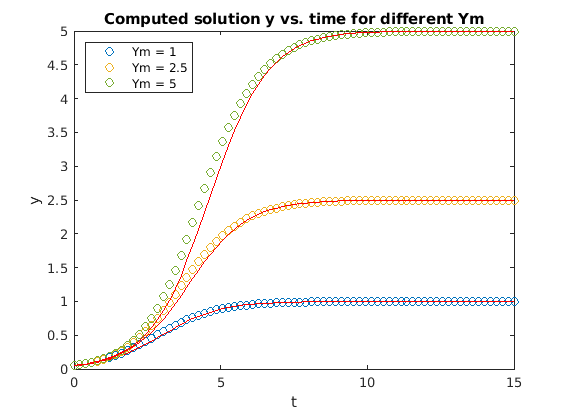
\includegraphics[width=0.7\columnwidth]{BackwardEulerLogistic.png}
	\caption{The solution to the logistic equation \cref{eq:ForwardEulerLogistic} computed using the backward Euler algorithm for three different $Y_m$ values.  Matlab's fsolve() was used to compute $y_{n+1}$ at each step of the method.  Note that the computed solution leads (is in front of) the analytic solution.  Compare these results to those for the forward Euler iteration in \cref{fig:ForwardEulerLogistic}}
	\label{fig:BackwardEulerLogistic}
\end{figure}


\section{Example: the simple harmonic oscillator}
To apply the backward Euler method to the simple harmonic oscillator we start with the pair of first order ODEs,
\begin{align}
\nonumber
\frac{d u}{d t} &= -\frac{k}{m} v  \\
\nonumber
\frac{d v}{d t} &= u
\end{align}
then discretize using the backward difference approximation.  We get
\begin{equation}
\label{eq:BackwardEulerSystem}
\begin{aligned}
\frac{u_{n+1} - u_{n}}{h} &= -\frac{k}{m} v_{n+1}  \\
\frac{v_{n+1} - v_{n}}{h} &= u_{n+1}
\end{aligned}
\end{equation}
Rearranging and moving the future to the LHS and the present to the RHS this becomes
\begin{align}
\nonumber
u_{n+1} + h \frac{k}{m} v_{n+1} = u_{n}  \\
\nonumber
v_{n+1} - h u_{n+1}= v_{n} 
\end{align}
Now we can gather the coefficients on the LHS into a matrix and write this as
\begin{align}
\nonumber
\begin{pmatrix}
1 & h k / m \\
-h & 1
\end{pmatrix}
\begin{pmatrix}
u_{n+1}  \\
v_{n+1} 
\end{pmatrix} = 
\begin{pmatrix}
u_{n}  \\
v_{n} 
\end{pmatrix}
\end{align}
As with forward Euler, we note that the system \cref{eq:BackwardEulerSystem} may be replaced with matrix-vector multiplication because the original equation is linear.  If the original system was nonlinear, then you would need to solve it as a system (i.e. you would not be able to simplify it into a matrix-vector multiplication form.)

We want to isolate the future on the LHS and use the RHS to compute the future using known quantities.  Therefore, we move the matrix to the RHS to get the iteration,
\begin{align}
\label{eq:BackwardEulerMatrixInverse}
\begin{pmatrix}
u_{n+1}  \\
v_{n+1} 
\end{pmatrix} = 
\begin{pmatrix}
1 & h k / m \\
-h & 1
\end{pmatrix}^{-1}
\begin{pmatrix}
u_{n}  \\
v_{n} 
\end{pmatrix}
\end{align}
Now we have isolated all the known quantities onto the RHS so we have a time-stepping method.  In the Matlab implementation we could use the analytic inverse of the $2 \times 2$ matrix, but instead we will just leave it as it stands and let Matlab perform the computation using a linear solve operation.  This is in the spirit of backward Euler, where each step of the algorithm involves inverting the function \cref{eq:BackwardEulerRootfinding} appearing on the LHS.  In this case, the function is matrix-vector multiplication, so we just need to invert the matrix (i.e. do a linear solve) to move it to the RHS.

Running the backward Euler SHO algorithm produces the the plot shown in \cref{fig:BackwardEulerSHOPropagator}.  In this case we find the sinusoidal oscillations decay with time.  For smaller step $h$ the decay is slower than for larger $h$.  Again, this behavior is not consistent with the analytic solution, which is a sine wave having constant amplitude -- that is, no increase nor decay with time.
\begin{figure}[tbh]
	\centering
	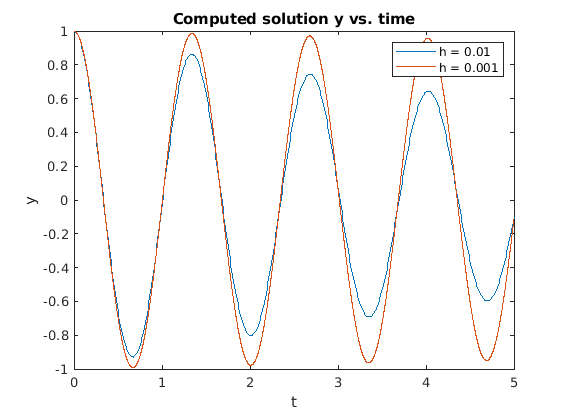
\includegraphics[width=0.7\columnwidth]{BackwardEulerSHOPropagator.png}
	\caption{The simple harmonic oscillator solved using backward Euler and a propagator matrix.  In contrast to the known mathematically-exact solution, the numerical solution decays exponentially in time.  The decay rate is faster for larger step sizes $h$.}
	\label{fig:BackwardEulerSHOPropagator}
\end{figure}

\subsection{Stability of backward Euler for the simple harmonic oscillator}
Understanding why the solution decays involves finding the eigenvalues of the propagator matrix.  That is, we will undertake a stability analysis for backward Euler similar to that presented in \cref{sect:FwdEulerSHOStability} for forward Euler.
To make life easy we'll first define
\begin{equation}
\label{eq:BackwardEulerPropagatorMatrix}
\omega^2 = \frac{k}{m}
\end{equation}
This just makes the algebra easier later.  Next, we invert the matrix on the RHS of \cref{eq:BackwardEulerMatrixInverse}.  This gives us the propagator matrix
\begin{equation}
\nonumber
\begin{pmatrix}
\frac{1}{h^2 \omega^2 + 1} & - \frac{h \omega^2}{h^2 \omega^2 + 1} \\
\frac{h}{h^2 \omega^2 + 1} & \frac{1}{h^2 \omega^2 + 1}
\end{pmatrix}
\end{equation}
To understand the stability of the iteration we must examine the eigenvalues of the propagator matrix \cref{eq:BackwardEulerPropagatorMatrix}.  Call the eigenvalues $g$ for "growth factor".  The eigenvalues of this matrix are found by solving
\begin{equation}
\nonumber
det
\begin{pmatrix}
	\frac{1}{h^2 \omega^2 + 1} - g & - \frac{h \omega^2}{h^2 \omega^2 + 1} \\
	\frac{h}{h^2 \omega^2 + 1} & \frac{1}{h^2 \omega^2 + 1} -g
\end{pmatrix}
=0
\end{equation}
for $g$.  We have
\begin{equation}
\nonumber
\left(\frac{1}{h^2 \omega^2 + 1} - g \right)^2 + \frac{h^2 \omega^2}{(h^2 \omega^2 + 1)^2} = 0
\end{equation}
so
\begin{equation}
\nonumber
g = \frac{1 \pm i h \omega}{h^2 \omega^2 + 1} 
\end{equation}
or
\begin{equation}
\label{eq:BackwardEulerSHOStability}
g = \frac{1}{1 \pm i h \omega} 
\end{equation}
Now consider the magnitude (absolute value) of $g$.  The numerator of \cref{eq:BackwardEulerSHOStability} is one while the denominator always has absolute value less than one.  Therefore, $|g| < 1$ always unless $h=0$ or $\omega=0$.  $h=0$ is not a useful value since it implies no stepping.  Therefore, for any reasonable value of $h \omega$ the solution obtained by backward Euler will always decrease for any non-zero stepsize $h$, as is observed in \cref{fig:BackwardEulerSHOPropagator}.



\section{Chapter summary}
Here are the important points made in this chapter:
\begin{itemize}
	\item The backward Euler method is derived from the simple backward difference expression for the derivative, $y' = (y_{n} - y_{n-1})/h$.
	\item The backward Euler method is an iterative method which starts at an initial point and walks the solution forward using the iteration 
	$y_{n+1} - h f(t_{n+1}, y_{n+1}) = y_{n}$.
	\item Since the future $y_{n+1}$ appears as a function which must be inverted on the LHS, backward Euler is an implicit method.
	\item Like any implicit method, a rootfinder -- such as Newton's method -- is required to find $y_{n+1}$ at each step in time.  
	\item The RMS error expected when using the backward Euler method scales as $e \sim O(h)$.
	\item Solver stability is not guaranteed for all step sizes $h$.  The stability criterion depends upon the exact ODE under consideration, but forward Euler can be stable for larger step sizes than forward Euler.
\end{itemize}

%%%%%%%%%%%%%%%%%%%%%%%%%%%%%%%%%%%%%%%%%%%%%%%%%%%%%%%%%%%%%%%%%%%%%%%%%%%%%%%%%%%%%%%%%%%%%%%%%%%%%%%%%%%%%%%%%%%%%%%%%%%
%%%%%%%%%%%%%%%%%%%%%%%%%%%%%%%%%%%%%%%%%%%%%%%%%%%%%%%%%%%%%%%%%%%%%%%%%%%%%%%%%%%%%%%%%%%%%%%%%%%%%%%%%%%%%%%%%%%%%%%%%
\chapter{Predictor-corrector methods and Runge-Kutta}

\section{Heun's method}
The next ODE solver is Heun's method.  It uses a new approach to computing the best step to take from the current position $(t_n, y_n)$.  To better appreciate Heun's method, let's first review the problems experienced by the two methods studied so far:
\begin{itemize}
	\item \textbf{Forward Euler.}  In forward Euler we compute the slope of $y(t)$ at the current time $t_n$ and use that slope to take a step forward into the future.  The problem with forward Euler is that the function $f(t, y)$ might curve away from the line predicted by the slope at $t_n$.  Consequently, forward Euler's accuracy is $O(h)$ -- which is low.
	\item \textbf{Backward Euler.}  Backward Euler uses the slope at time $t_{n+1}$ to compute the forward step.  Once again, however, the solution $y(t)$ can curve away from the line predicted by the slope at $t_{n+1}$, so the accuracy is again low.
\end{itemize}
The problem with both methods is that they use a linear approximation to the behavior of the solution inside the interval $t_n \le t \le t_{n+1}$, and use a slope computed at the end of the interval.  Heun's method tries to fix this problem by retaining the linear approximation, but averaging the slopes from both ends of the domain.  Specifically, Heun's method does the following:
\begin{enumerate}
	\item Sit at $t=t_n$ and compute the slope at this point, $s_1 = f(t_n, y_n)$.
	\item Use this slope to estimate the solution's value at $t_{n+1}$ using standard forward Euler:  $\tilde{y}(t_{n+1}) = y(t_n) + h f(t_n, y_n)$.  Note we denote this point $\tilde{y}(t_{n+1})$ using a tilde $\sim$ since it's an intermediate step towards our solution.
	\item At this point $(t_n, \tilde{y}_{n+1})$ compute the slope $s_2 = f(t_{n+1}, \tilde{y}_{n+1})$.
	\item Average these two slopes to compute the forward step:
	\begin{equation}
	 y(t_{n+1} ) = y(t_n) + \frac{h}{2} \left( s_1 + s_2 ) \right)
	\end{equation}
\end{enumerate}
The method still assumes a straight-line approximation to $y(t)$ in the interval $t_n \le t \le t_{n+1}$ but uses a better approximation to the slope. The formal algorithm is presented in \cref{alg:Heun}.
\begin{algorithm}
	\caption{Heun's method}
	% Must put label after caption for cref to work.
	\label{alg:Heun}
	\begin{algorithmic} 
		\STATE {Inputs: initial condition $y_0$, end time $t_{end}$.}
		\STATE {Initialize: $t_0=0$, $y_0$.} 
		\FOR{$n=0:t_{end}/h$} 
		\STATE Compute slope at $t_n$: $S_1 \leftarrow f(t_n, y_n)$
		\STATE Compute intermediate step at $t_{n+1}$: $\tilde{y} \leftarrow y_n + h S_1$
		\STATE Compute slope at $t_{n+1}$: $S_2 \leftarrow f(t_{n+1}, \tilde{y})$
		\STATE Compute final step: $y_{n+1} \leftarrow y_n + (h/2)(S_1 + S_2)$
		\ENDFOR
		\RETURN $y$ vector.
	\end{algorithmic}
\end{algorithm}
This process is shown graphically in \cref{fig:HeunsMethod}.  
\begin{figure}[tbh]
	\centering
	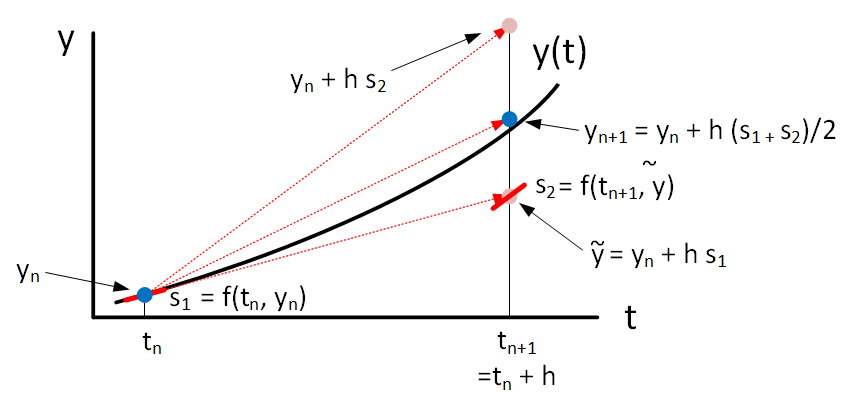
\includegraphics[width=0.8\columnwidth]{HeunsMethod.png}
	\caption{Heun's method first computes an intermediate value at $t_{n+1}$ which we call $\tilde{y}$ using forward Euler.  It then uses this value to compute the slope at $t_{n+1}$.  It then averages the two slopes at $t_n$ and $t_{n+1}$ to compute the actual step.}
	\label{fig:HeunsMethod}
\end{figure}
The plot shows the result of computing $y_{n+1}$ using forward and backward Euler as well as Heun's method.  The thing to observe is that for the function curvature shown, forward Euler undershoots the actual function value at $y_{n+1}$ and backward Euler overshoots it.  However, since Heun's method averages the present and (guessed) future slopes, it comes much closer to hitting the desired correct value of $y_{n+1}$.

Heun's method is perhaps the most basic ODE solver in a large family of solvers which are called "predictor-corrector" methods.  The idea is that these methods first take one or more "predictor" steps into the future, then use the results of the predictor steps to compute the "corrector" -- the actual step.  In the case of Heun's method we have:
\begin{itemize}
	\item Predictor: $\tilde{y} = y_n + h f(t_n, y_n)$
	\item Corrector: $y_{n+1} = y_n + (h/2)(f(t_n, y_n) + f(t_{n+1}, \tilde{y}))$
\end{itemize}
In some sense, these intermediate $y$ values are used to "feel" what the slope looks in the future.  Once enough trial steps have been taken (predictor step), then they are combined together (corrector step) to form the final step.

\section{Example: the exponential growth ODE and error scaling}
As usual, we examine the result of using Heun's method on the exponential growth ODE, \cref{eq:ForwardEulerExponential}.  Simulation results are shown in \cref{fig:HeunsMethodExponential}.  The computed solution clearly gives a better match to the analytic results -- Heun's method is a better method than forward Euler!
\begin{figure}[tbh]
	\centering
	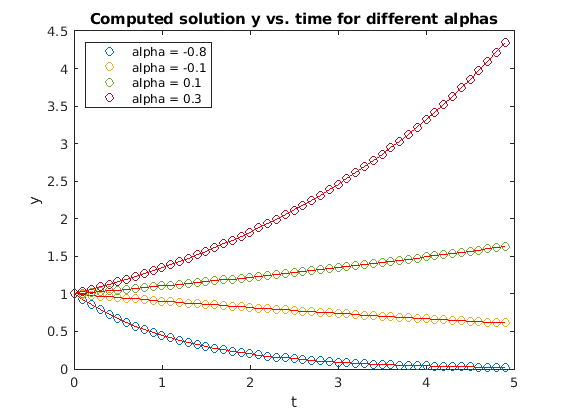
\includegraphics[width=0.7\columnwidth]{HeunsMethodExponential.png}
	\caption{The exponential growth ODE \cref{eq:ForwardEulerExponential} solved using Heun's method.  The fit between the computed solution and the analytic solution is clearly better than that for forward Euler.}
	\label{fig:HeunsMethodExponential}
\end{figure}
We can quantify the accuracy of Heun's method by computing the RMS error between the computed and the analytic solutions for different stepsizes $h$.  This is shown in \cref{fig:HeunsMethodExponentialErr}.  On a log-log plot the slope of the error line is two -- the order of Heun's method is accordingly $O(h^2)$.  That is, if we halve the stepsize then we get a factor of four improvement in method accuracy.  This is much better than the $O(h)$ accuracy offered by forward Euler.
\begin{figure}[tbh]
	\centering
	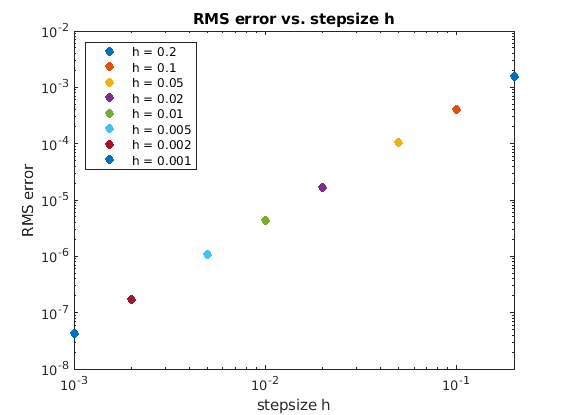
\includegraphics[width=0.7\columnwidth]{HeunsMethodExponentialErr.png}
	\caption{Scaling of the RMS error of \cref{eq:ForwardEulerExponential} for Heun's method.  Examining the slope of the curve shows that the error incurred by Heun's method scales as $e \sim O(h^2)$.}
	\label{fig:HeunsMethodExponentialErr}
\end{figure}



\section{Example: the simple harmonic oscillator}
Our friend the simple harmonic oscillator is also easy to implement using Heun's method.  The result of running Heun's method using a larger step size than used for both forward and backward Euler is shown in \cref{fig:HeunsMethodSHO}.  
\begin{figure}[tbh]
	\centering
	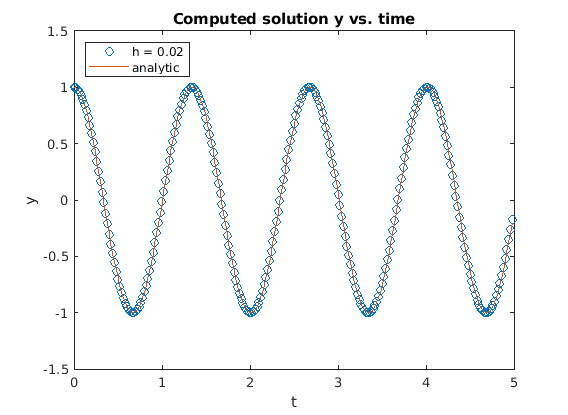
\includegraphics[width=0.7\columnwidth]{HeunsMethodSHO.png}
	\caption{The simple harmonic oscillator solved using Heun's method. Open circles are the computed result for $h=0.2$ and the line is the analytic result.  The computed result matches the analytic result much better than for the Euler methods, at least at this plot scale.  This is because Heun's method is order $O(h^2)$.}
	\label{fig:HeunsMethodSHO}
\end{figure}
Compared to both forward and backward Euler, the oscillation neither grows nor decays significantly over the 5 second simulation time -- at least on the scale of \cref{fig:HeunsMethodSHO}.  This suggests Heun's method is a superior algorithm to both forward and backward Euler.  The better accuracy is a result of using slope information from both time $t_n$ as well as $t_{n+1}$ -- this gives the method an $h^2$ order.  Nonetheless, all is not rosy -- see \cref{fig:HeunsMethodSHODiff} which plots the difference between the computed and the analytic solution.  The difference evidently grows exponentially, although the magnitude is not as bad as with the Euler methods.
\begin{figure}[tbh]
	\centering
	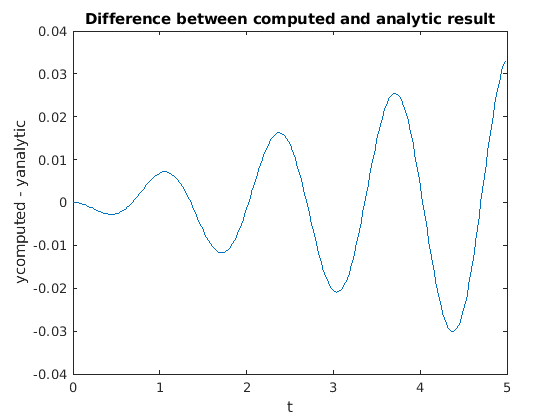
\includegraphics[width=0.7\columnwidth]{HeunsMethodSHODiff.png}
	\caption{The difference between the computed and the analytic result shown in \cref{fig:HeunsMethodSHO}. The difference is small, but grows exponentially.}
		\label{fig:HeunsMethodSHODiff}
	\end{figure}


\section{Midpoint method}
A similar method to Heun's is the midpoint method.  We will specifically look at the explicit midpoint method (there is also an implicit midpoint method).  The midpoint method uses forward Euler to take a half-step forward, then computes the slope at that point and uses that slope to make the full step.  The algorithm is presented in \cref{alg:Midpoint}.
\begin{algorithm}
	\caption{Midpoint method}
	% Must put label after caption for cref to work.
	\label{alg:Midpoint}
	\begin{algorithmic} 
		\STATE {Inputs: initial condition $y_0$, end time $t_{end}$.}
		\STATE {Initialize: $t_0=0$, $y_0$.} 
		\FOR{$n=0:t_{end}/h$} 
		\STATE Compute slope at $t_n$: $s_1 \leftarrow f(t_n, y_n)$
		\STATE Compute intermediate step to $t_{n} + h/2$: $\tilde{y} \leftarrow y_n + (h/2) s_1$
		\STATE Compute slope at $t_{n} + h/2$: $s_2 \leftarrow f(t_{n}+h/2, \tilde{y})$
		\STATE Compute final step: $y_{n+1} \leftarrow y_n + h s_2$
		\ENDFOR
		\RETURN $y$ vector.
	\end{algorithmic}
\end{algorithm}
A drawing showing how the midpoint method works is shown in \cref{fig:MidpointMethod1}.
\begin{figure}[tbh]
	\centering
	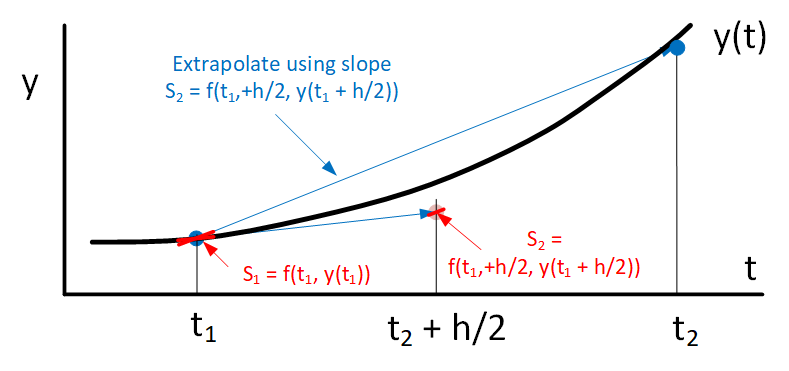
\includegraphics[width=0.7\columnwidth]{MidpointMethod1.png}
	\caption{The midpoint method.}
	\label{fig:MidpointMethod1}
\end{figure}


\section{Example: the exponential growth ODE}
We examine the midpoint method on the exponential growth ODE, \cref{eq:ForwardEulerExponential}.  Simulation results are shown in \cref{fig:MidpointMethodExponential}.  The computed solution clearly gives a better match to the analytic results than forward Euler -- the midpoint method is also a better method than forward Euler!
\begin{figure}[h]
	\centering
	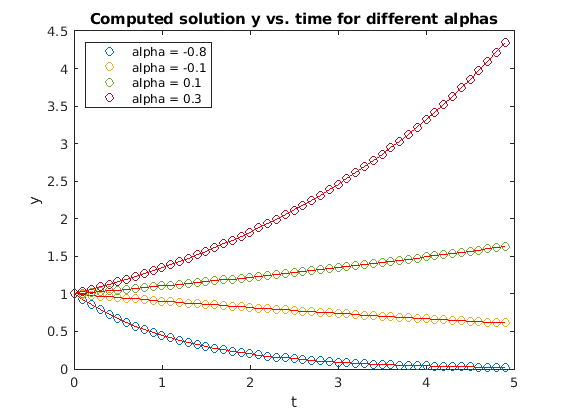
\includegraphics[width=0.7\columnwidth]{MidpointMethodExponential.png}
	\caption{The exponential growth ODE \cref{eq:ForwardEulerExponential} integrated using the midpoint method.  The fit between the computed solution and the analytic solution is again better than that for forward Euler.}
	\label{fig:MidpointMethodExponential}
\end{figure}
The RMS error vs. stepsize plot is shown in \cref{fig:MidpointMethodExponentialErr}.  On a log-log plot the slope of the error line is two -- this says that the order of the method is $O(h^2)$.
\begin{figure}[h]
	\centering
	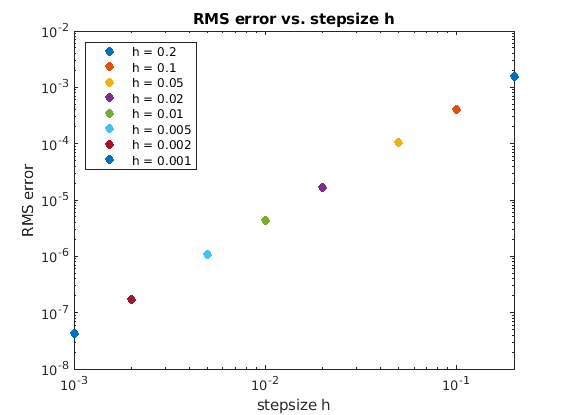
\includegraphics[width=0.7\columnwidth]{MidpointMethodExponentialErr.png}
	\caption{Scaling of the RMS error of \cref{eq:ForwardEulerExponential} for the midpoint method.  The RMS error scales as $e \sim O(h^2)$.}
	\label{fig:MidpointMethodExponentialErr}
\end{figure}



\section{Runge-Kutta methods}
\label{sect:RK4}
The most famous predictor-corrector methods are the Runge-Kutta methods.  Even if you have had only passing familiarity with numerical methods for ODEs in the past, you have probably heard of these methods, or even used them!  In particular, 4th-order Runge-Kutta is the most common workhorse used when solving ODEs.  It is the go-to solver used to solve the majority of ODEs.  A variant of 4th-order Runge-Kutta is built into Matlab as the function ode45.  There are plenty of other ODE solvers available, but one generally tries 4th order Runge-Kutta first, and if it doesn't work or produces poor results then one turns to other, more specialized methods.

We will concentrate on the classic 4th order Runge-Kutta method since it is the most common one.  Runge-Kutta methods of other orders also exist, but this 4th order method is both most common and also shows all the relevant concepts you should learn.  In any event, you will likely call a pre-written solver from a library in your real work, so the important thing to learn are the concepts involved, not the details of each and every variant in the Runge-Kutta family.

In what follows we will call this particular variant of 4th order Runge Kutta "RK4" for brevity.  RK4 takes four samples of the present and future slopes.  Here is the method:
\begin{align}
	\nonumber
    k_1 &= h f(t_n, y_n) \\
	\nonumber
	k_2 &= h f(t_n+h/2, y_n + k_1/2) \\
	\nonumber
	k_3 &= h f(t_n+h/2, y_n + k_2/2) \\
	\nonumber
	k_4 &= h f(t_n+h, y_n + k_3) \\
	\nonumber
	y_{n+1} &= y_n + (k_1 + 2 k_2 + 2 k_3 + k_4)/6
\end{align}
Things to note about RK4:
\begin{itemize}
	\item RK4 computes four intermediate results, $k_1$, $k_2$, $k_3$, $k_4$.  Each intermediate result relies on the preceeding computation -- that means you must perform the computations in order.  The computation is depicted graphically in \cref{fig:RungeKuttaSamplePoints}.
	\item The final result is a weighted sum of the intermediate results.
	\item RK4 is an explicit method -- no rootfinding is required to compute the desired result.
	\item You might wonder where the sample points and the coefficients in the weighted sum come from.  The short answer is, they are something you look up in a book (or online).  The longer answer is, of course they may be derived, but the derivation is long and tedious and doesn't lend any insight into the method.  Therefore, we will skip the derivation here.
	\item We have depicted $y$ to be a scalar in the above -- that is, we assumed we are solving a single, scalar ODE.  However, just as in the previous methods, $y$ may also be a vector -- that is, RK4 may also  be used to solve a system of ODEs in the same way as may be used for all previous methods.
\end{itemize}
\begin{figure}[tbh]
	\centering
	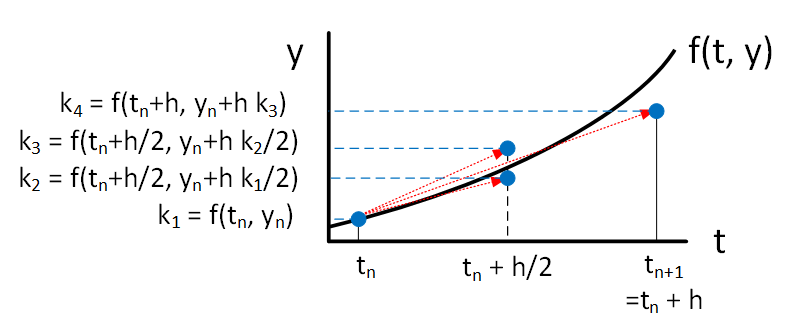
\includegraphics[width=0.7\columnwidth]{RungeKuttaSamplePoints.png}
	\caption{Fourth order Runge-Kutta intermediate results depicted graphically.  The method relies on sampling the slope of the function $f(t, y)$ at four different locations in order to compute the final step.  The sample locations are built up sequentially.  Note that two of the locations lie one-half way between the current time $t_n$ and the final time $t_{n+1}$.}
	\label{fig:RungeKuttaSamplePoints}
\end{figure}


\section{Example: the exponential growth ODE}
We examine using RK4 on the usual exponential growth ODE, \cref{eq:ForwardEulerExponential}.  Simulation results are shown in \cref{fig:RK4Exponential}.  The computed solution matches the analytic result closely.
\begin{figure}[tbh]
	\centering
	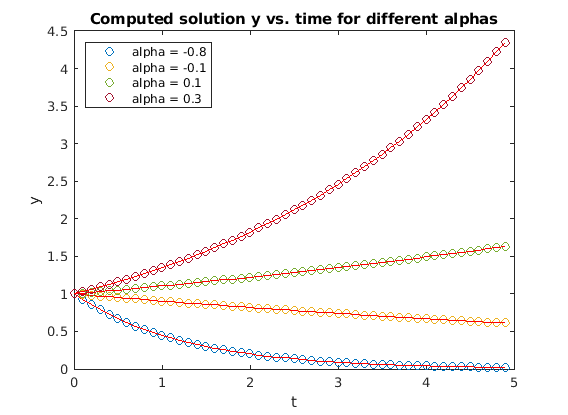
\includegraphics[width=0.7\columnwidth]{RK4Exponential.png}
	\caption{The exponential growth ODE \cref{eq:ForwardEulerExponential} integrated using fourth-order Runge-Kutta (RK4).  The fit between the computed solution and the analytic solution is again better than that for forward Euler.}
	\label{fig:RK4Exponential}
\end{figure}
The RMS error vs. stepsize plot is shown in \cref{fig:RK4ExponentialErr}.  This time the slope on a log-log plot is four -- this says that the order of the method is $O(h^4)$.
\begin{figure}[tbh]
	\centering
	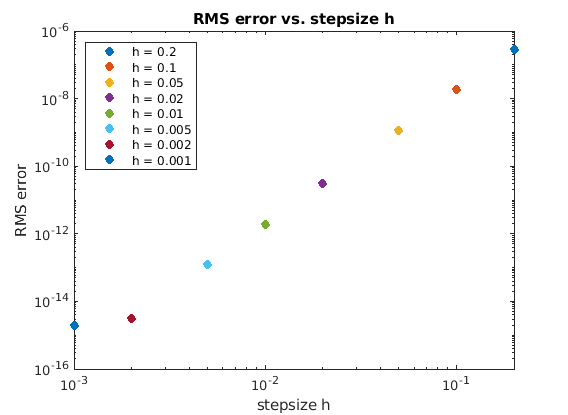
\includegraphics[width=0.7\columnwidth]{RK4ExponentialErr.png}
	\caption{RMS error of the exponential growth ODE \cref{eq:ForwardEulerExponential} for RK4 for varying $h$.  The RMS error for RK4 scales as $e \sim O(h^4)$ which is excellent.  (The leftmost point doesn't fall on the line.  However, note that its value is around 1e-15 -- a typical value for a small quantity corrupted by round-off error.)}
	\label{fig:RK4ExponentialErr}
\end{figure}


\section{Example: the simple harmonic oscillator}
Let's explore using RK4 using our old friend the SHO.  Once again broken down into two first order ODEs, the SHO is
\begin{align}
\nonumber
\frac{d u}{d t} &= -\frac{k}{m} v  \\
\nonumber
\frac{d v}{d t} &= u
\end{align}
To use RK4 we write this in the general form
\begin{equation}
\begin{aligned}
\frac{d u}{d t} &= f(t, u, v)  \\
\frac{d v}{d t} &= g(t, u, v)
\end{aligned}
\label{eq:RK4SHOSystem}
\end{equation}
with $f(t, u, v) = -(k/m) v$ and $g(t, u, v) = u$.  
To implement this method on the computer we treat all variables as vectors.  That is, we gather the LHS expression as
\begin{equation}
\nonumber
y = 
\begin{pmatrix}
du/dt \\
dv/dt
\end{pmatrix} 
\end{equation}
and the RHS as
\begin{equation}
\nonumber
F = 
\begin{pmatrix}
f(t, u, v) \\
g(t, u, v)
\end{pmatrix} 
\end{equation}
so the vectorized system to integrate is
\begin{equation}
\nonumber
\frac{dy}{dt} = 
F(t, y)
\end{equation}
Then each of the intermediate steps $k_i$ is a $2 \times 1$ column vector.  Writing the problem this way makes it easy to implement RK4 using vectorized expressions.  Results obtained for integrating the SHO using RK4 are shown in \cref{fig:RK4SHO} alongside the analytic result $\cos(\omega t)$.  The results look great -- both $h = 0.1$ and $h=0.01$ produce cosine waves which look picture-perfect -- at least over the scale and time period simulated.  However, the results are not perfect -- \cref{fig:RK4SHODiff} shows the difference (error) between the computed and the analytic results.  Although the difference is small, it is nonzero.  Worse, the error grows exponentially with increasing time.  This suggests the RK4 method -- like forward and backward Euler -- is unstable for the simple harmonic oscillator, albeit much better than the other methods.
\begin{figure}[tbh]
	\centering
	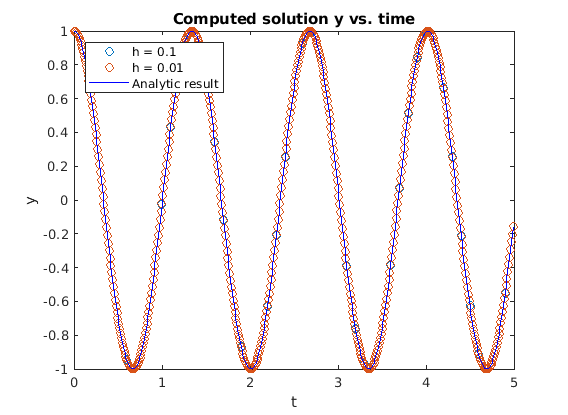
\includegraphics[width=0.7\columnwidth]{RK4SHO.png}
	\caption{The simple harmonic oscillator solved using 4th order Runge-Kutta.  The open circles are the computed results and the solid line is the analytic result.  At this scale the results look perfect to the eye.}
	\label{fig:RK4SHO}
\end{figure}
\begin{figure}[tbh]
	\centering
	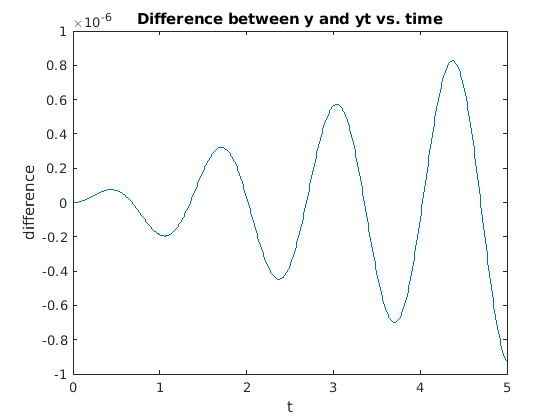
\includegraphics[width=0.7\columnwidth]{RK4SHODiff.png}
	\caption{The difference between the computed result for $h = 0.01$ and the analytic result $\cos(\omega t)$.  The difference is very small, but still grows with increasing time.}
	\label{fig:RK4SHODiff}
\end{figure}

\section{Example: the hanging pendulum}
We have employed the simple harmonic oscillator as a useful example to demonstrate the different solvers encountered so far.  The SHO is sometimes used as a linearized model of the motion of a hanging pendulum.  However, a real hanging pendulum's motion is governed by a nonlinear ODE.  The geometry of the problem is shown in \cref{fig:RealHangingPendulum}.  
\begin{figure}[tbh]
	\centering
	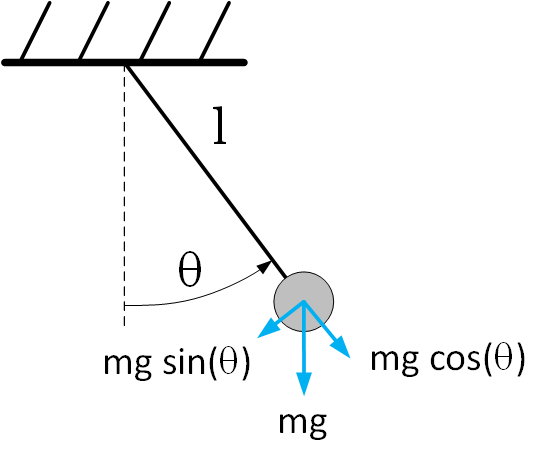
\includegraphics[width=0.3\columnwidth]{RealHangingPendulum.png}
	\caption{The real hanging pendulum.}
	\label{fig:RealHangingPendulum}
\end{figure}
The independent variable is time $t$, the dependent variable (which we want to solve for) is the angle $\theta$ made by the pendulum with respect to vertical.  The pendulum's length is $l$ and the gravitational force constant is $g$.  The ODE is derived as follows:
\begin{enumerate}
	\item We consider the forces acting on the pendulum when it is displaced from the vertical by an angle $\theta$.  In particular, gravity pulls the pendulum down with a constant vertical force $m g$.
	\item The vertical force may be resolved into two components:  One in the $\hat{r}$ direction -- in line with the pendulum's support, and one in the $\hat{\theta}$ direction.  Elementary trig says the force in the $\hat{\theta}$ direction is $F_{\theta} = -m g \sin(\theta)$.  The negative sign appears since the force pulls the pendulum bob back to the equilibrium point at $\theta = 0$.
	\item Newton's second law states $F = m a$.  In the case of the pendulum bob, $F$ is the force acting in the $\hat{\theta}$ direction, and $a$ is the acceleration in the $\hat{\theta}$ direction.  Since the pendulum bob is attached to the rod of length $l$, the angular acceleration is $l d^2 \theta / d t^2$.
	\item Using the above information, the equation governing the pendulum's motion is
	\begin{equation}
	\nonumber
	m l \frac{d^2 \theta}{d t^2} = -m g \sin(\theta)
	\end{equation}
	or 
	\begin{equation}
	\label{eq:NonlinearPendEq}
	\frac{d^2 \theta}{d t^2} = -\frac{g}{l} \sin(\theta)
	\end{equation}
\end{enumerate}
Observe that for small $\theta$ we may approximate $\sin(\theta) \approx \theta$ which gives back the SHO.  But for large pendulum swings this approximation doesn't work and we need to use the full, non-linear expression for the restoring force on the pendulum bob.  In this case an analytic solution for \cref{eq:NonlinearPendEq} exists -- the analytic solution may be expressed using the Jacobi elliptic functions sn and cn.  However, rather than playing around with higher transcendental functions, we'll just use RK4 to compute the solutions numerically.

To proceed, we break the second order ODE \cref{eq:NonlinearPendEq} into two first order ODEs.  We get
\begin{align}
\label{eq:NonlinearPendEqTwoODEs}
\nonumber
\frac{du}{dt} &= v \\
\nonumber
\frac{dv}{dt} &= -\frac{g}{l} \sin(u)
\end{align}
Now we rearrange this system into a vector form for use with the Runge-Kutta implementation.  We get
\begin{equation}
\begin{aligned}
\label{eq:NonlinearPendEqVectorized}
\begin{pmatrix}
du/dt \\
dv/dt
\end{pmatrix} 
=
\begin{pmatrix}
v \\
-(g/l) \sin(u)
\end{pmatrix} 
\end{aligned}
\end{equation}
This form is ready for implementation.  The vectorized form \cref{eq:NonlinearPendEqVectorized} is
implemented in a function called by the RK4 integrator itself, and a test wrapper is the main program run by the user.  This is the usual software architecture previously shown in \cref{fig:ForwardEulerArch}.

Running the RK4 implementation gives the plot shown in \cref{fig:RealHangingPendulumRK4}.  This plot was obtained using $g = 9.8$ m/sec$^2$ (the value of $g$ at the earth's surface) and $l = 0.5$m, a reasonable value for the length of a pendulum.  For initial conditions, the pendulum swing started with the bob pointing almost vertically up.  Therefore, the pendulum takes a long time for the bob to accelerate.  It then swings quickly around the downward hanging position and continues until pointing almost vertically up again.  The pendulum then repeats this motion again and again, never stopping because the original equation does not include any dissipation (friction).
\begin{figure}[tbh]
	\centering
	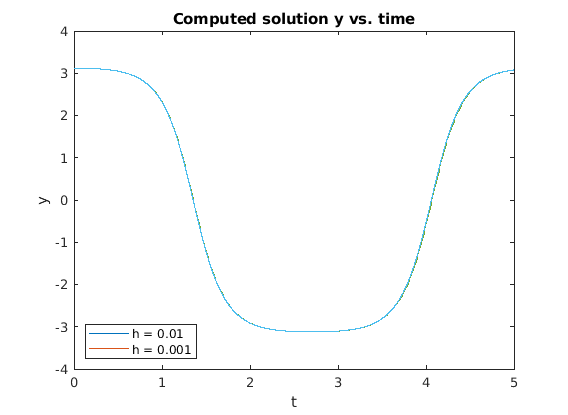
\includegraphics[width=0.7\columnwidth]{RealHangingPendulumRK4.png}
	\caption{The hanging pendulum ODE solved using RK4.  This plot shows the motion of the pendulum when the bob starts pointing almost vertically up.}
	\label{fig:RealHangingPendulumRK4}
\end{figure}


\section{Example: the Van der Pol oscillator}
In the 1920, the Dutch physicist  Balthasar van der Pol was employed by Philips to work on vacuum tubes.  Vacuum tubes were electronic devices used to amplify signals in the days before transistors.  Van der Pol found that under certain circumstances the vacuum tubes would spontaneously oscillate on their own.  Uncontrolled self-oscillations are a very undesirable behavior, so he was interested in understanding why they happened.  Van der Pol investigated the physical reasons for the oscillation and determined that the voltage swing across the vacuum tube could be modeled by the second order ODE 
\begin{equation}
\label{eq:VanDerPolOsc}
\frac{d^2 y}{d t^2} - \epsilon(1 - y^2)\frac{d y}{d t} + y = 0
\end{equation}
where $y$ is the voltage across the tube.  The $\epsilon$ term represents a non-linear damping since it involves the $d y/d t$ term.  When $y < 1$ this term represents amplification: it imparts a positive value to ${d^2 y}/{d t^2}$ when ${d y}/{d t}$ is also positive, thereby the amplitude of the oscillation increases.  When $y > 1$ the opposite happens:  the term adds a negative value to ${d^2 y}/{d t^2}$ for positive ${d y}/{d t}$ causing the amplitude of the oscillation to decrease.   Therefore, the action of the $\epsilon$ term is to create an oscillation whose amplitude remains bounded in time.

This second order ODE may be broken into two first order ODEs by defining
\begin{align}
\nonumber
u &=  y \\
\nonumber
v &= \frac{d y}{d t}
\end{align}
Then, the ODE system is  
\begin{align}
%\label{eq:VanDerPolOscSystem}
\nonumber
\frac{d u}{d t } &= v \\
\nonumber
\frac{d v}{d t} &= \epsilon(1 - u^2) v - u
\end{align}
Integrating this system using RK4 gives the plot shown in \cref{fig:RK4VanDerPol}.  
\begin{figure}[tbh]
	\centering
	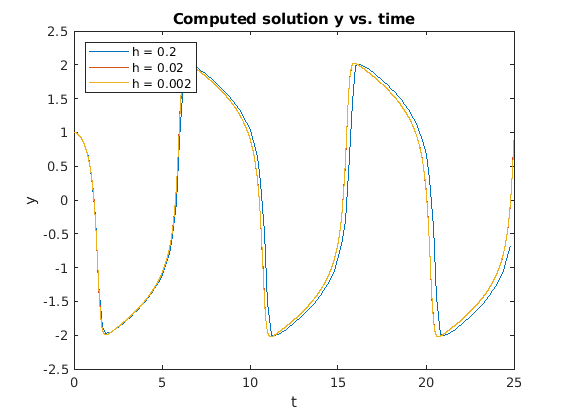
\includegraphics[width=0.7\columnwidth]{RK4VanDerPol.png}
	\caption{The Van der Pol oscillator solved using RK4.  For this plot the coefficient $\epsilon = 3.5$.  }
	\label{fig:RK4VanDerPol}
\end{figure}
Things to note about the results shown in \cref{fig:RK4VanDerPol}:
\begin{itemize}
	\item As predicted, after a quick start-up phase, the Van der Pol ODE produces a constant amplitude, periodic oscillation.  We note that the oscillation looks nothing like the usual sin or cosine oscillations produced by linear oscillators.  The strong nonlinearity introduced by the $dy/dt$ term is the reason for behind this shape.
	\item Note that the $h=0.2$ curve is displaced from the curves generated with smaller $h$ values.  This is a real effect.  \Cref{eq:VanDerPolOsc} is a so-called "stiff" ODE, which makes it difficult to solve numerically, at least using larger step sizes.  This property will be detailed in section \cref{sect:StiffODEs} below.
\end{itemize}

\section{Example: Duffing's equation}
Duffing's equation is a nonlinear variant of the simple harmonic oscillator.  It models the situation where the spring's response is not linear for all extensions, but rather the spring's restoring force grows faster than linearly at the ends of the spring's travel.  This models the real-world behavior of springs -- springs don't behave linearly if you pull on the spring to the end of it's extent.  Duffing's equation models the stiffness by adding a cubic term to the restoring force.  For small displacements the cubic force is small, but for larger displacements it will dominate the return force.  On the RHS, Duffing also adds a drive force -- in this case a cosine drive of frequency $\omega$.  
A drawing of the physical setup is shown in \cref{fig:DuffingsEq}.
\begin{figure}[tbh]
	\centering
	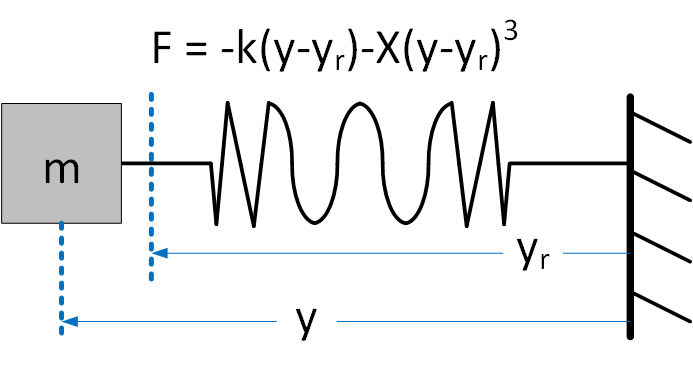
\includegraphics[width=0.7\columnwidth]{DuffingsEq.png}
	\caption{Duffing's equation models the situation where the spring's response is not linear, but rather becomes stiffer at the ends of the travel range.}
	\label{fig:DuffingsEq}
\end{figure}
The full Duffing's equation is
\begin{equation}
\label{eq:DuffingsEq}
\frac{d^2 y}{d t^2} + \delta \frac{d y}{d t} + \alpha y + \beta y^3 = \gamma \cos(\omega t)
\end{equation}

\begin{figure}[tbh]
	\centering
	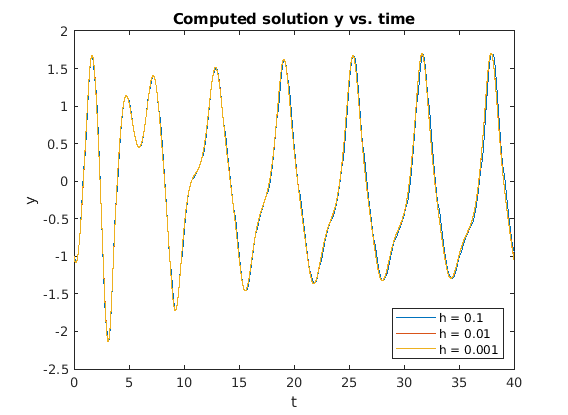
\includegraphics[width=0.7\columnwidth]{RK4Duffings.png}
	\caption{Duffing's equation solved using RK4.}
	\label{fig:RK4Duffings}
\end{figure}

\section{Butcher tableaux}
As mentioned above, there are many different variants of the Runge-Kutta method itself, as well as other types of predictor-corrector methods.  A useful device which catalogs the different methods are the Butcher tableaux.  These are tables summarizing the different coefficients which make up a particular method.  A general, explicit predictor-corrector method looks like this:
\begin{equation}
\begin{aligned}
\label{eq:GeneralPredCor}
k_1 =& h f(t_n, y_n) \\
k_2 =& h f(t_n + c_2 h, y_n + a_{21} k_1) \\
k_3 =& h f(t_n + c_3 h, y_n + a_{31} k_1 + k_{32} k_2) \\
 & \vdots \\
y_{n+1} =& y_n + \left( b_1 k_1 + b_2 k_2 + b_3 k_3 + \cdots \right)
\end{aligned}
\end{equation}
Compare this to the definition of RK4 shown above.  A Butcher tableau summarizes the coefficients as shown the \cref{tab:GeneralButcherTableau}.
\begin{table}[h]
	\begin{center}
		\renewcommand{\arraystretch}{1.5}
		\begin{tabular}{  c|c c c c } 
			$c_1$ & $a_{11}$ & $a_{12}$ & $a_{13}$ & $\cdots$ \\ 
			$c_2$ & $a_{21}$ & $a_{22}$ & $a_{23}$ & $\cdots$ \\ 
			$c_3$ & $a_{31}$ & $a_{32}$ & $a_{33}$ & $\cdots$ \\ 
			$\vdots$ & $\vdots$ & $\vdots$ & $\vdots$ & $\ddots$ \\ 
			\hline
			 & $b_1$ & $b_2$ & $b_3$ & $\cdots$ \\ 
		\end{tabular}
		\caption{Definition of the Butcher tableau.  The coefficients are those shown in \cref{eq:GeneralPredCor}.}\label{tab:GeneralButcherTableau}
	\end{center}
\end{table}
\FloatBarrier 
As examples, Butcher tableaux for Heun's method, the midpoint method, and RK4 are shown in \cref{tab:Heun} - \cref{tab:ButcherRK4}.  Compare the coefficients in the tables against the definitions of the solver methods to see how they are related.
\begin{center}
\begin{minipage}{2in}
	\begin{center}
	\begin{tabular}{c|cc}
		0 & 0 & 0 \\
		1 & 1 & 0 \\
		\hline
		 & 1/2 & 1/2 \\
	\end{tabular}
	\end{center}
	\begin{align}
		\nonumber
		k_1 &= h f(t_n, y_n) \\
		\nonumber
		k_2 &= h f(t_n+h, y_n + k_1) \\
		\nonumber
		y_{n+1} &= y_n + k_1/2 + k_2/2
	\end{align}
	\captionof{table}{Heun's method}\label{tab:Heun}
\end{minipage}
\begin{minipage}{2in}
	\begin{center}
	\begin{tabular}{c|cc}
		0 & 0 & 0 \\
		1/2 & 1/2 & 0 \\
		\hline
		& 0 & 1 \\
	\end{tabular}    
	\end{center}
	\begin{align}
		\nonumber
		k_1 &= h f(t_n, y_n) \\
		\nonumber
		k_2 &= h f(t_n+h/2, y_n + k_1/2) \\
		\nonumber
		y_{n+1} &= y_n + k_2
	\end{align}
	\captionof{table}{Midpoint method}\label{tab:Midpoint}
\end{minipage}
\end{center}

\begin{center}
\begin{minipage}{4in}
		\begin{center}
		\renewcommand{\arraystretch}{1.5}
		\begin{tabular}{  c|c c c c } 
			0 & 0 & 0 & 0 & 0 \\ 
			1/2 & 1/2 & 0 & 0 & 0 \\ 
			1/2 & 0 & 1/2 & 0 & 0 \\ 
			1 & 0 & 0 & 1 & 0 \\ 
			\hline
			& 1/6 & 1/3 & 1/3 & 1/6 \\ 
		\end{tabular}
		\end{center}
	\begin{align}
	\nonumber
	k_1 &= h f(t_n, y_n) \\
	\nonumber
	k_2 &= h f(t_n+h/2, y_n + k_1/2) \\
	\nonumber
	k_3 &= h f(t_n+h/2, y_n + k_2/2) \\
	\nonumber
	k_4 &= h f(t_n+h, y_n + k_3) \\
	\nonumber
	y_{n+1} &= y_n + (k_1 + 2 k_2 + 2 k_3 + k_4)/6
	\end{align}
\captionof{table}{Fourth-order Runge-Kutta}\label{tab:ButcherRK4}
\end{minipage}
\end{center}



\section{Chapter summary}
Here are the important points made in this chapter:
\begin{itemize}
	\item Predictor-corrector methods "feel" the slope at different times in the future in order to compute the best step forward in time.
	\item Heun's method and the midpoint method are simple examples of predictor-corrector methods.  Both are $O(h^2)$ methods.
	\item The workhorse method used to solve a large fraction of ODEs in the world is 4th order Runge-Kutta.  This method is the first thing you should try when faced with a new ODE if you don't have any special knowledge about the ODE's properties.
	\item As you might expect from its name, the RMS error of 4th order Runge-Kutta scales as $O(h^4)$.
	\item All methods shown in this chapter are explicit.
	\item Butcher tableaux are used to catalog the many different predictor-corrector methods by presenting their coefficients in a tabular form.
\end{itemize}

\chapter{Adaptive stepping}
\section{Choosing $h$}
Up until now I have not said much about what stepsize $h$ to choose.  Of course, accuracy and stability considerations suggest a smaller stepsize is usually better than a larger one.  However, if your stepsize is too small, then your program will take longer to run than necessary to get an accurate answer.  There is a trade-off between runtime and stepsize.  Runtime doesn't matter much when running the toy programs used to demonstrate the different methods in this booklet, but if you are doing a gigantic, real-world calculation then you don't want to waste time if you don't have to.  Oftentimes, the runtime of your program is important -- if your program is meant to predict tomorrow's weather but your program takes 48 hours to run, then your program is useless.

As a first step, if you know something about your ODE, and in particular know the timescale on which you expect to see the solution change, then choosing a stepsize to fit that time scale is easy.  However, you commonly don't know much about your solution's behavior, which is why you are simulating it in the first place.  Also, your ODE might behave badly -- the solution might be smooth and slowly-varying for one period of time, then become bursty or quickly-varying at a subsequent time.  Because of this, adaptive stepping is a common method useful to find the best stepsize for your simulation.  The idea is simple:
\begin{enumerate}
	\item Take a single step of size $h$.
	\item Estimate the error between the true solution and your step.
	\item If the error is too large, then go back and retry your step with a smaller stepsize, for example $h/2$.  Then use this step size moving forward.
	\item However, if the error is small enough, increase the stepsize for future steps.
	\item Go back to 1 and continue stepping.
\end{enumerate}
The idea is that the error incurred at each step can stay below some bound.  In rough terms, if your solution changes slowly then you may take larger steps.  But if your solution changes quickly, then you need to take smaller steps in order to maintain good accuracy.

Of course, the big question is, how to estimate the error?  In the best case you could compare your computed solution against the true solution -- but if you already had the true solution then you wouldn't need to run an ODE solver in the first place!  As a second-best case, you could use a so-called "oracle".  In computer science, an oracle is a function or a program you can ask if your solution is true or not.  That is, you can compute a step, then give the result to an oracle and it will say either "yes, your solution is correct" or "no, your solution is wrong".  As a thought-experiment the oracle is generally regarded as a "black box", meaning that you don't necessarily know how it works on the inside.  It's enough to simply know that the oracle will either say "yes" or "no" to your proposed answer, and the oracle will give an accurate judgement.

What is a good oracle for use with an ODE solver?   Here are two possibilities:
\begin{enumerate}
\item A simple idea is to just run each step twice: first use stepsize $h$, then take two steps of stepsize $h/2$ and compare the results.  In this case, the $h/2$ steps may be regarded as a sort of oracle since its answer is (presumably) more accurate than the $h$ step.  The problem with this scheme is that you effectively run the solver twice -- two times for each step.  This makes your program run (at least) twice as long as necessary.
\item You could also consider taking a step using, say, forward Euler, and then taking the same step using, say, Heun's method.  The idea here is that since forward Euler is $O(h)$ but Heun's method is $O(h^2)$ then Heun's method is a good oracle.  Again, this means you waste significant time recomputing your step.  On the other hand, in Heun's method you can reuse the initial forward Euler step, so you get back some some performance through reuse of previously computed results.
\end{enumerate}
It turns out that real-world solvers use a variant of possibility 2.  Recall the fourth-order Runge-Kutta method from \cref{sect:RK4}.  The RK4 method presented there is a member of a larger family of Runge-Kutta methods of varying order.  Matlab's famous ode45() solver uses a method called Dormand-Prince order 4/5.  In this solver, two Runge-Kutta methods are used.  The first is a 4th-order Runge-Kutta variant (not the one presented in \cref{sect:RK4}), and the second is a 5th-order Runge-Kutta method.  The coefficients used to compute the intermediate steps of both methods are the same, only the final computation is different.  Therefore, the amount of additional computation required to implement the oracle check is a small part of the overall calculation at each step.  The combined Butcher tableau of the methods used in ode45() are shown in \cref{tab:DP45ButcherTableau1}. 
\begin{table}
\begin{center}
	\renewcommand{\arraystretch}{1.5}
	\begin{tabular}{  c|c c c c c c c } 
		0 & 0 & 0 & 0 & 0 & 0  & 0  & 0  \\ 
		1/5 & 1/5 & 0 & 0 & 0 & 0  & 0  & 0  \\ 
		3/10 & 3/40 & 9/40 & 0 & 0 & 0 & 0 & 0 \\ 
		4/5 & 44/45 & -56/15 & 32/9 & 0 & 0 & 0 & 0 \\ 
		8/9 & 19372/6561 & -25360/2187 & 64448/6561 & -212/729 & 0 & 0 & 0 \\
		1 & 9017/3168 & -355/33 & 46732/5247 & 49/176 & -5103/18656 & 0 & 0 \\
		1 & 35/384 & 0 & 500/1113 & 125/192 & -2187/6784 & 11/84 & 0 \\
		\hline
		& 35/384 & 0 & 500/1113 & 125/192 & -2187/6784 & 11/84 & 0 \\ 
		& 5179/57600 & 0 & 7571/16695 & 393/640 & -92097/339200 & 187/2100 & 1/40 \\ 
		
	\end{tabular}
\caption{Butcher tableau for the Dormand-Prince 4/5 solver used in Matlab's ode45().  The two rows below the horizontal line correspond to the two corrector steps which are compared against each other.}
\label{tab:DP45ButcherTableau1}
\end{center}
\end{table}
You can also see these parameters in Matlab by issuing the command "dbtype 201:213 ode45", which emits the Butcher table in a slightly different form than above.
% 
%\begin{verbatim}
%>> dbtype 201:213 ode45
%201   % Initialize method parameters.
%202   pow = 1/5;
%203   A = [1/5, 3/10, 4/5, 8/9, 1, 1]; % Still used by restarting criteria
%204   % B = [
%205   %     1/5         3/40    44/45   19372/6561      9017/3168       35/384
%206   %     0           9/40    -56/15  -25360/2187     -355/33         0
%207   %     0           0       32/9    64448/6561      46732/5247      500/1113
%208   %     0           0       0       -212/729        49/176          125/192
%209   %     0           0       0       0               -5103/18656     -2187/6784
%210   %     0           0       0       0               0               11/84
%211   %     0           0       0       0               0               0
%212   %     ];
%213   % E = [71/57600; 0; -71/16695; 71/1920; -17253/339200; 22/525; -1/40];
%\end{verbatim}

Regarding changing the step size, my naive suggestion in item 1 either halves or doubles the step size depending upon the error measured by the method.  A better approach would be to tune the step size depending upon the magnitude of the observed error.  That is, make the new step size depend upon the actual error observed instead of blindly halving or doubling the step.  Algorithms for doing such fine-tuning exist, but are outside the scope of this booklet.

\section{Example:  the logistic equation}
Instead of demonstrating the full Dormand-Prince 4/5, I will show a simpler adaptive stepper based on possibility 2 above.  The program algorithm is shown in \cref{alg:NaiveAdaptiveStep}.  I use the logistic equation as the example because the solution has (roughly) two regions of interest:  A quickly varying phase of exponential growth at the beginning of the run followed by a plateau as $t \rightarrow \infty$.   Results obtained from the Matlab implementation of the program are shown in \cref{fig:AdaptiveEHLogistic}.  The step size clearly remain small during the beginning of the run, but when the solution stabilizes (doesn't change) the step size increases.  This is particularly evident for times $t > 10$.
\begin{figure}[bh]
	\centering
	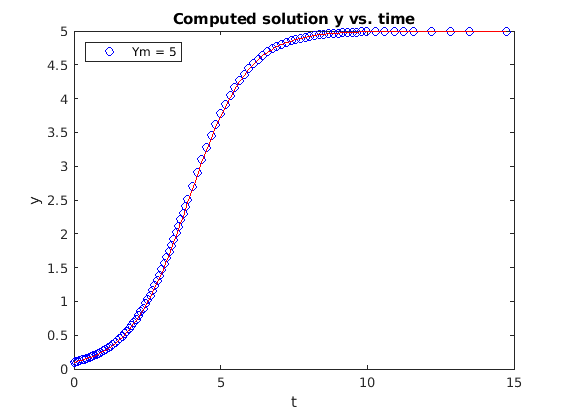
\includegraphics[width=0.7\columnwidth]{AdaptiveEHLogistic.png}
	\caption{Example run of my naive adaptive step solver on the logistic ODE.  This solver computes a forward Euler step, then computes a Heun's method step to use as the oracle.  When the results of the two steps disagree, the solver halves the stepsize and tries again.  When the steps agree closely, the solver doubles the stepsize for the next step.  Otherwise the solver continues iterating using the current step.  The step size increases for slowly-varying portions of the solution are evident at times $t > 10$.   The red line is the analytic solution.}
	\label{fig:AdaptiveEHLogistic}
\end{figure}
\begin{algorithm}
	\caption{Naive adaptive step method}
	\label{alg:NaiveAdaptiveStep}
	\begin{algorithmic} 
		\STATE {Inputs: initial condition ${y_0} = [u_0, v_0]^T$, end time $t_{end}$.}
		\STATE {Initialize: $t_0=0$, ${y_0}$, $h$.} 
		\STATE {Initialize: $tol_1 = 1e-2$, $tol_2 = 2e-4$.}
		\FOR{$n=0:t_{end}/h$} 
		\STATE Get inital slope: $s_1 = f(t_n, y_n)$
		\STATE Take forward Euler step: $y_{fe} = y_n + h s_1$
		\STATE Get slope at new position: $s_2 = f(t_n, y_{fe})$
		\STATE Take Heun step: $y_h = y_n + h (s_1+s_2)/2$
		\STATE Check difference between Euler and Heun steps: $\delta = ||y_{fe}-y_h||$
		
		\IF { $\delta > tol_1$ }
		\STATE Error too large -- decrease step: $h = h/2$
		\ELSIF { $\delta < tol_2$ }
		\STATE Error very small -- increase step: $h = 2 h$
  		\ELSE
		\STATE Error neither too small or too large.  Keep step.
		\ENDIF
		
		\ENDFOR
		\RETURN ${y_n}$.
	\end{algorithmic}
\end{algorithm}


\section{Stiff ODEs}
\label{sect:StiffODEs}
In the last section we saw an adaptive step method which took small steps when the solution varied quickly, and took larger steps when the solution varied slowly.  The concept of slow vs. fast varying generalizes to the concept of "stiffness" of an ODE.  An exact definition of the term "stiff" is hard to pin down, but the basic intuition is that a stiff ODE is one where you need to take small steps at some times to maintain accuracy, but can take much larger steps at other times.  The problem with a stiff ODE is that if you use a fixed time step $h$, then you need $h$ to be very small for those sections of the ODE requiring small steps.  However, stepping then proceeds slowly over sections where you could use a large $h$ and step quickly -- meaning you are wasting compute time!  Dealing with stiffness is why adaptive solvers are so important.

The Van der Pol equation is a common example of a stiff ODE.  The solution computed using the adaptive stepper is shown in \cref{fig:AdaptiveEHVanDerPol}.  When the solution peaks out at around $y \approx \pm 2$ the step size must decrease significantly to maintain an accurate solution.  Inspecting the phase plot \cref{fig:AdaptiveEHVanDerPolPhase} shows another view of this phenomenon -- when the solution takes a hard right turn the step size must decrease to follow the solution, but the step size may increase when the solution moves away from the "right turn".
\begin{figure}[h]
	\centering
	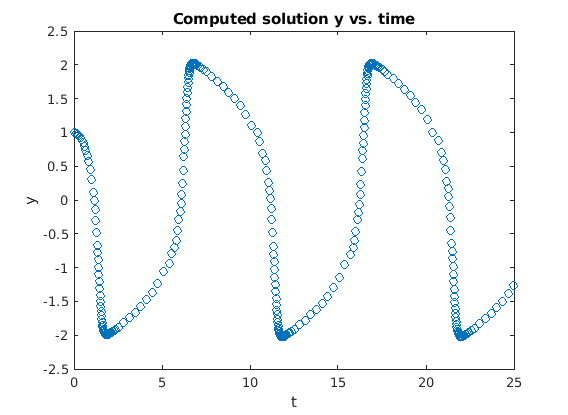
\includegraphics[width=0.7\columnwidth]{AdaptiveEHVanDerPol.png}
	\caption{The Van der Pol equation integrated using my naive adaptive step solver.  Note that the solver takes small steps at the "corners" where the solution saturates at a value $y \approx \pm 2$.}
	\label{fig:AdaptiveEHVanDerPol}
\end{figure}
\begin{figure}[h]
	\centering
	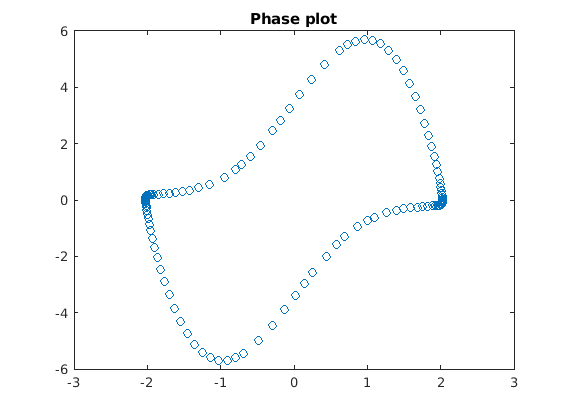
\includegraphics[width=0.7\columnwidth]{AdaptiveEHVanDerPolPhase.png}
	\caption{The phase plot shows that the stepsizes decrease where the solution takes a hard right turn, but increase when the solution moves away from the "corners".}
	\label{fig:AdaptiveEHVanDerPolPhase}
\end{figure}
The question is, why does the step size need to decrease at these points in the phase plane, but not in others?  The answer comes from considering the entire family of solutions to the Van der Pol equation in the phase plane.  A plot of the situation is shown in \cref{fig:VanDerPolPhasePlots}, which is a phase plot for varying values of $\epsilon$.  The solutions for varying $\epsilon$ are bunched together at the corners, but spread out away from those regions.  Near the corners staying on the correct solution (i.e. not jumping to another solution in the family) depends very sensitively upon closely following the correct solution trajectory.  The adaptive stepper somehow "feels" this sensitivity and accordingly adjusts the step size to remain on the correct trajectory. 
\begin{figure}[th]
	\centering
	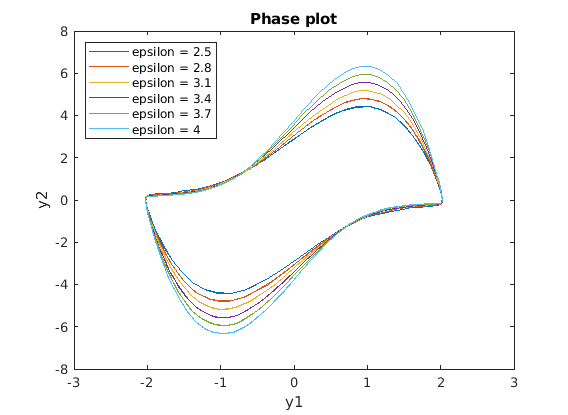
\includegraphics[width=0.7\columnwidth]{VanDerPolPhasePlots.png}
	\caption{Phase plots for varying values of $\epsilon$.  Note that the solutions are bunched together in the vicinity of the "corners".  This signals that finding the correct solution from all solutions in the family depends very sensitively upon the details of the solution trajectory.  Small perturbations cause potentially large changes in the trajectory.  The adaptive stepper somehow "feels" this sensitivity and accordingly adjusts the step size to remain on the correct trajectory. }
	\label{fig:VanDerPolPhasePlots}
\end{figure}
The importance of adaptive step size solvers is simply that if the solver did not change its step size, then to get an accurate solution you would need to use a very small step $h$ to remain on the correct trajectory in the sensitive regions.  The sensitive regions are those where the family of solutions lies close to one another.  However, small $h$ means the solver's run time would be much longer than needed since it would also take small steps through the region where the solution trajectory is relatively insensitive.  The adaptive solver is the best of both cases:  Fast stepping through the insensitive regions and slow, careful stepping through the sensitive regions.
\section{Chapter summary}
Here are the important points made in this chapter:
\begin{itemize}
	\item An adaptive step size method changes the step size $h$ to maintain the solution error remains below some tolerance.  When the stepper senses the solution error is growing, it will decrease the step size until the error resulting from a step remains below the tolerance.  When the stepper senses that the solution error is small enough, it will increase the step size to speed up the solution.
	\item A stiff system is one in which the solution evidences regions of fast and regions of slow variation, or more exactly high or low sensitivity to adjacent solutions to the ODE.   
\end{itemize}

\chapter{Linear multistep methods}
The cannonical form of a first order ODE is given in \cref{eq:basicODE}.  Until now, the ODE solver algorithms we have examined started from approximating the derivative operator in \cref{eq:basicODE}, then building on that approximation to create a solver.  
\begin{equation}
\label{eq:basicODE}
\frac{dy}{dt} = f(t, y)
\end{equation}
Now we'll try a different approach.  Instead of starting from the derivative, think about how we might construct an ODE solver by integrating both sides of \cref{eq:basicODE} and then creating a stepping method.  Specifically, consider the equation
\begin{equation}
\label{eq:integratedODE}
y_{n+1} = \int_{t_n}^{t_{n+1}} f(t, y(t)) dt + y_n
\end{equation}
This equation is derived from \cref{eq:basicODE} by integration.  The problem with doing the integration directly is that the RHS requires knowledge of $y(t)$ -- the thing we are trying to find!  But what happens if we chose an approximation for $f$ and do the integration?  It turns out that different multistep methods are created by using different approximations for $f$.  We'll look at a few methods in this chapter.

\section{Trapezoidal method}
A simple approximation to $f$ in \cref{eq:integratedODE} is to assume that points $(t_n, f_n)$ and $(t_{n+1}, f_{n+1})$ are connected via a straight line.  This is the case of linear interpolation between two points and is shown in \cref{fig:TrapezoidalMethod}
\begin{figure}[h!]
	\centering
	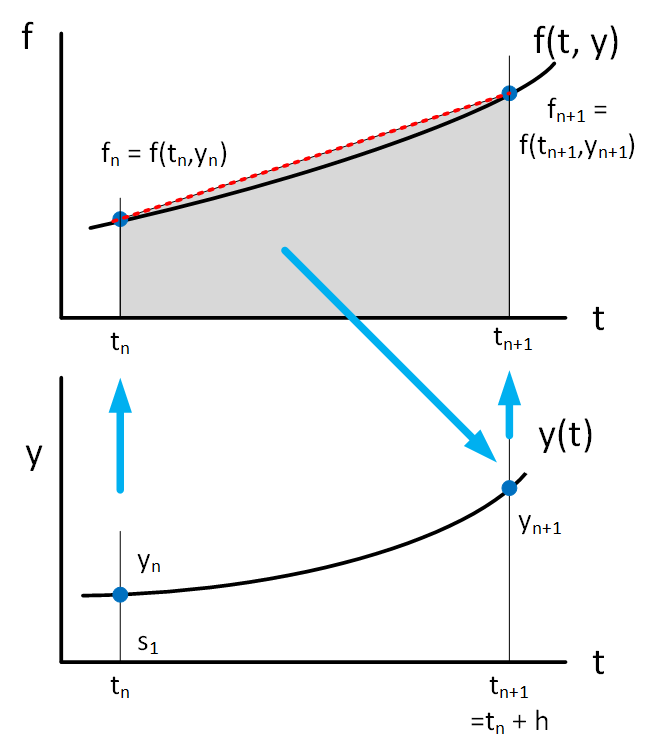
\includegraphics[width=0.6\columnwidth]{TrapezoidalMethod.png}
	\caption{The trapezoidal method.  The red dotted line is the linear interpolation.  The grey region corresponds to the "area under the curve" which is computed by the integral \cref{eq:IntegrateLinearInterp}.  Note this method is implicit.}
	\label{fig:TrapezoidalMethod}
\end{figure}
Linear interpolation between $t_n$ and $t_{n+1}$ may be written in this form:
\begin{equation}
\label{eq:LinearInterpolation}
f(t) = (1-\alpha) f_n + \alpha f_{n+1}
\end{equation}
where $\alpha \in [0, 1]$.  Obviously, when $\alpha = 0$ we get $f(t) = f_n$ and when $\alpha = 1$ we get $f(t) = f_{n+1}$.  Since \cref{eq:LinearInterpolation} is linear in $\alpha$, this expression draws a straight line between these two points.

Now consider what happens if we use the interpolation method \cref{eq:LinearInterpolation} in the integral \cref{eq:integratedODE}.  To make the algebra easier we recognize $\alpha = (t - t_n)/h$ so that $h d\alpha = dt$.  In this case, \cref{eq:integratedODE} becomes
\begin{equation}
\label{eq:IntegrateLinearInterp}
y_{n+1} = h \int_{0}^{1} \left( (1-\alpha) f_n + \alpha f_{n+1} \right) d \alpha + y_n
\end{equation}
which integrates to
\begin{equation}
\label{eq:TrapezoidalMethod}
y_{n+1} = \frac{h}{2} \left( f_{n+1} + f_n \right) + y_n
\end{equation}
This is an iteration which takes us from $t_n$ to $t_{n+1}$.  
Here are some things to note about \cref{eq:TrapezoidalMethod}:
\begin{itemize}
	\item This is an implicit method -- to get $y_{n+1}$ on the LHS you need to know $f_{n+1}$ which depends upon $y_{n+1}$.  Fortunately, we already know how to deal with implicit methods -- use a rootfinder like Newton's method.
	\item The equation whose root to find is $g(y_{n+1}) = y_{n+1} -\frac{h}{2} \left( f_{n+1} + f_n \right) - y_n = 0$ where $f_{n+1} = f(t_{n+1}, y(t_{n+1}))$ and $f_{n} = f(t_{n}, y(t_{n}))$ as usual.
	\item This method has approximated $f(t)$ using a straight line between the two end points, and then integrated the approximation.  This is exactly the same as the "trapezoidal method" for numerical integration which you may have seen in a previous numerical analysis class.  Therefore, this ODE solver is called the "trapezoidal method".
\end{itemize}

\section{Example: the exponential growth ODE}
\begin{figure}[tbh]
	\centering
	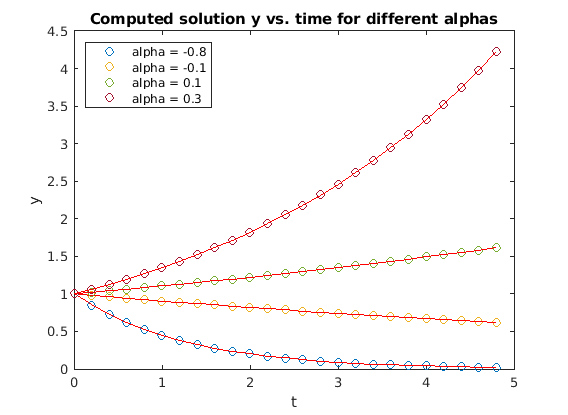
\includegraphics[width=0.60\columnwidth]{TrapezoidalExponential.png}
	\caption{The exponential growth ODE integrated using the trapezoidal method.  The open circles are the computed results, the lines are the analytic solution.  The fit is pretty good, at least on this scale.}
	\label{fig:TrapezoidalExponential}
\end{figure}
\begin{figure}[h!]
	\centering
	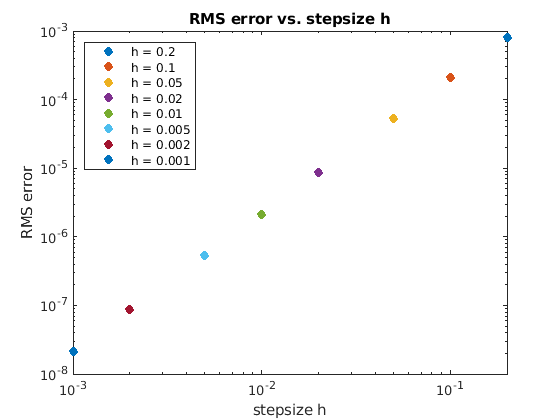
\includegraphics[width=0.60\columnwidth]{TrapezoidalExponentialErr.png}
	\caption{Error scaling of the trapezoidal method.  The error scales as $O(h^2)$.}
	\label{fig:TrapezoidalExponentialErr}
\end{figure}


\section{Adams-Bashforth method -- 2nd order}
The trapezoidal method uses linear interpolation between points at $t_n$ and $t_{n+1}$.  It is an implicit method, meaning that it assumes we know the end value $y_{n+1}$ in order to compute the step using $f_{n+1} = f(t_{n+1}, y_{n+1})$.  However, the step computation is what is used to get the end value $y_{n+1}$.  Therefore, computing the step requires a solve operation to untangle $y_{n+1}$ from $f_{n+1}$.  A solve operation is generally expensive -- solvers like Newton's method are iterative and one might need several iterations before the solution is found.  Wouldn't it be better to somehow use the linear interpolation to create an explicit method requiring no solver step?

The explicit 2nd order Adams-Bashforth method is such a method.  It uses the known (previously computed) values at times $t_n$ and $t_{n+1}$ to compute the value at $t_{n+2}$.  The idea is shown in \cref{fig:AdamsBashforth2}.  
\begin{figure}[tbh]
	\centering
	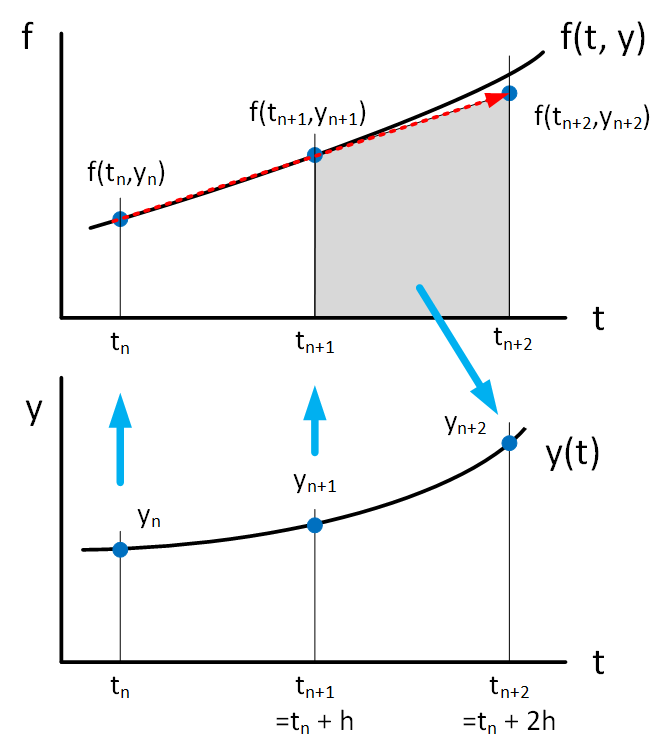
\includegraphics[width=0.6\columnwidth]{AdamsBashforth2.png}
	\caption{The 2nd order Adams-Bashforth method.  First, linear interpolation is performed between the points $(t_n, y_n)$ and $(t_{n+1}, y_{n+1})$.  Then the line is extended to $t_{n+2}$ and the grey region under the curve is integrated per \cref{eq:AdamsBashforthIntegral1} to give the new value $y_{n+2}$.}
	\label{fig:AdamsBashforth2}
\end{figure}
In a sense, Adams-Bashforth takes the interpolation formula \cref{eq:LinearInterpolation} defined on $t \in [t_n, t_{n+1}]$ and extrapolates it forward to time $t_n+2$.  That is, it computes the integral 
\begin{equation}
\label{eq:AdamsBashforthIntegral}
y_{n+2} = \int_{t_{n+1}}^{t_{n+2}} f_{n, n+1}(t, y(t)) dt + y_{n+1}
\end{equation}
using the approximation to $f_{n, n+1}$ based on the linear interpolation formula defined on $t \in [t_n, t_{n+1}]$, \cref{eq:LinearInterpolation}.  We transform the integral \cref{eq:AdamsBashforthIntegral} via the usual change of variables $\alpha = (t - t_n)/h$ to get
\begin{equation}
\label{eq:AdamsBashforthIntegral1}
y_{n+2} = h \int_{1}^{2}  \left( (1-\alpha) f_n + \alpha f_{n+1} \right) d \alpha  + y_{n+1}
\end{equation}
Upon integration we get the second order Adams-Bashforth method,
\begin{equation}
\label{eq:AdamsBashforthSecondOrder}
y_{n+2} = h \left( \frac{3}{2} f_{n+1} - \frac{1}{2} f_{n} \right)   + y_{n+1}
\end{equation}
Notice that second-order Adams-Bashforth uses two samples of the function at $t_n$ and $t_{n+1}$ to compute the future value at $t_{n+2}$.  This is an explicit method since we presumably already know $f_{n+1}$ and $f_n$ when computing $f_{n+2}$.  But this begs the question, how to start this iteration?  That is, we have only one initial condition, $y_0$, but need two $y$ values to iterate.  The answer is that one can start with $y_0$, then use a single step of e.g. forward Euler or Runge-Kutta to get $y_1$, then continue the solution using Adams-Bashforth.  This is the method employed in the Matlab program whose output is shown in \cref{fig:AdamsBashforth2Exponential}.  Note that the accuracy is $O(h^2)$, as expected from a second-order method.
\begin{figure}[tbh]
	\centering
	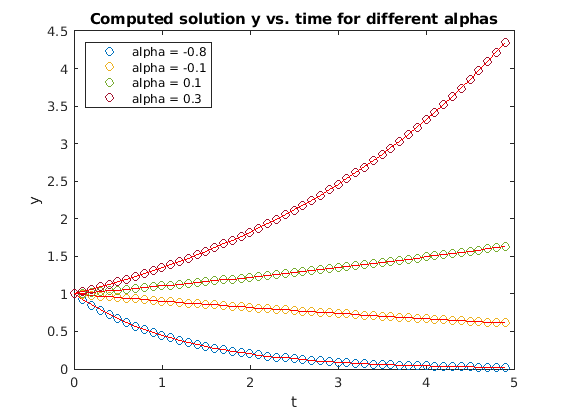
\includegraphics[width=0.7\columnwidth]{AdamsBashforth2Exponential.png}
	\caption{The exponential growth ODE integrated using 2nd order Adams-Bashforth.}
	\label{fig:AdamsBashforth2Exponential}
\end{figure}
\begin{figure}[tbh]
	\centering
	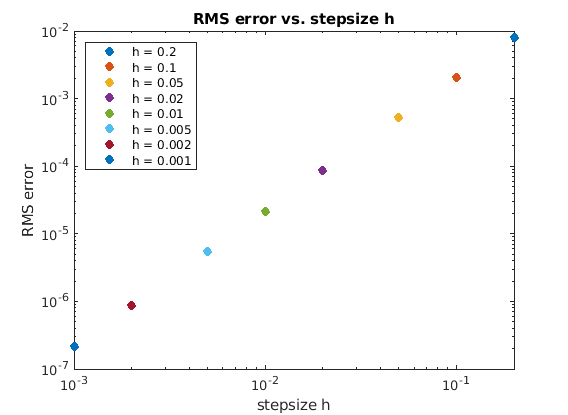
\includegraphics[width=0.7\columnwidth]{AdamsBashforth2ExponentialErr.png}
	\caption{Error scaling of 2nd order Adams-Bashforth.  The error scales as $O(h^2)$.}
	\label{fig:AdamsBashforth2ExponentialErr}
\end{figure}

\section{Adams-Bashforth method -- 3rd order}
The second-order Adams-Bashforth method used linear interpolation to approximate the function $f(t,y)$ over the interval $t_n \le t \le t_{n+1}$, then used that approximation in the integral \cref{eq:integratedODE} to find $y_{n+1}$.  What if you want more accuracy?  Can you use quadratic interpolation on three past points to find the future value?  The answer is "yes", and the advantage to this is that the order of the method increases.  In this section we will derive the third-order Adams-Bashforth method (quadratic interpolation).  

Given two points $(t_n, y_n)$ and $(t_{n+1}, y_{n+1})$ we can draw a straight line through them.  Given three points, we can draw a quadratic (a parabola) through them.  This is the process of interpolation which you have likely studied in a previous math class.  Given a set of points, there are several ways to write down an interpolating polynomial which passes through them.  In this case, we are given three points, $(t_n, y_n)$, $(t_{n+1}, y_{n+1})$, and $(t_{n+2}, y_{n+2})$, and we will use the Lagrange interpolation polynomial to write down the quadratic.  It is
\begin{gather}
\label{eq:LagrangeInterpolation}
\nonumber
f(t) = \frac{(t-t_{n+1})(t-t_{n+2})}{(t_{n}-t_{n+1})(t_{n}-t_{n+2})} f_{n}
+\frac{(t-t_{n})(t-t_{n+2})}{(t_{n+1}-t_{n})(t_{n+1}-t_{n+2})} f_{n+1} \\
\nonumber
+\frac{(t-t_{n})(t-t_{n+1})}{(t_{n+2}-t_{n})(t_{n+2}-t_{n+1})} f_{n+2}
\end{gather}
\begin{equation}
\label{eq:LagrangeInterpolation1}
\nonumber
= \frac{(t-t_{n+1})(t-t_{n+2})}{2 h^2} f_{n}
+\frac{(t-t_{n})(t-t_{n+2})}{-h^2} f_{n+1}
+\frac{(t-t_{n})(t-t_{n+1})}{2 h^2} f_{n+2}
\end{equation}
This expression might look nasty, but note that it is just a quadratic:  Every term is second order in $t$.  Now we insert this expression into the integral \cref{eq:integratedODE} to find $y_{n+3}$:  
\begin{equation}
\nonumber
y_{n+3} = \int_{t_{n+2}}^{t_{n+3}} 
\frac{(t-t_{n+1})(t-t_{n+2})}{2 h^2} f_{n}
+\frac{(t-t_{n})(t-t_{n+2})}{-h^2} f_{n+1}
+\frac{(t-t_{n})(t-t_{n+1})}{2 h^2} f_{n+2}
dt 
+ y_n
\end{equation}
The thing to note is that we use previous points $(t_{n}, y_{n})$, $(t_{n+1}, y_{n+1})$, $(t_{n+2}, y_{n+2})$ to create an approximate version of $f(t, y)$ using interpolation.  Then we integrate that approximation over the interval $t \in [t_{n+2}, t_{n+3}]$ to get $y_{n+3}$.  The method is shown schematically in \cref{fig:AdamsBashforth3}.
\begin{figure}[tbh]
	\centering
	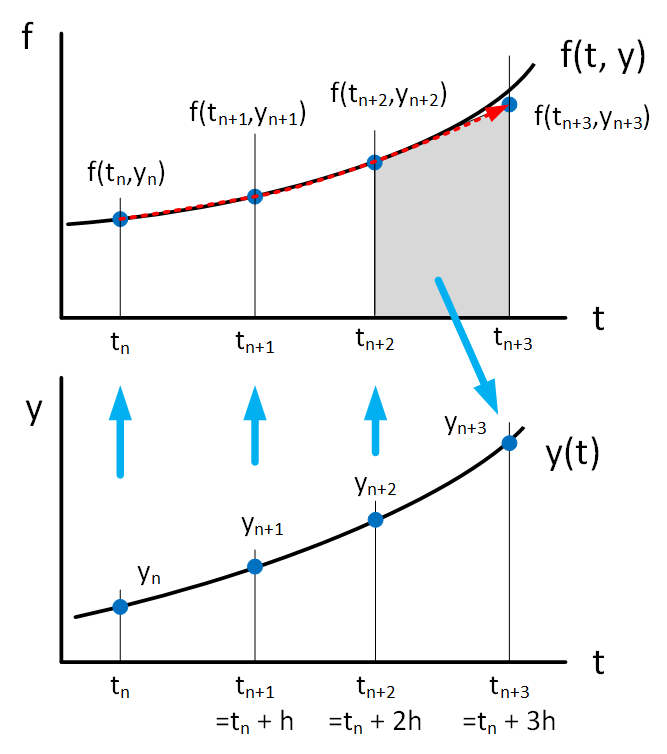
\includegraphics[width=0.7\columnwidth]{AdamsBashforth3.png}
	\caption{The 3rd-order Adams-Bashforth method.  The upward pointing blue arrows indicate that the three points $f_n$, $f_{n+1}$ and $f_{n+2}$ are known and are used to create the quadratic interpolation polynomial for $f(t,y)$ (red dotted line).  That polynomial is integrated from $t_{n+2}$ to $t_{n+3}$ to get the new $y$ value, $y_3$.}
	\label{fig:AdamsBashforth3}
\end{figure}
We could carry out the integration immediately, but it would be rather messy.  Therefore, we employ the usual change of variables $\alpha = (t - t_{n+1})/h$.  Note that $h d\alpha = dt$, and that we have mapped $t = t_{n} \rightarrow \alpha = -1$, $t = t_{n+1} \rightarrow \alpha = 0$, $t = t_{n+2} \rightarrow \alpha = 1$, and $t = t_{n+3} \rightarrow \alpha = 2$.  Therefore, the integral becomes
 \begin{equation}
 \nonumber
 y_{n+3} = h \int_{1}^{2} 
\frac{1}{2} \alpha(\alpha-1) f_{n}
 -(\alpha+1)(\alpha-1) f_{n+1}
 +\frac{1}{2} (\alpha+1)\alpha f_{n+2}
 d\alpha
 + y_n
 \end{equation}
 or
  \begin{equation}
  \label{eq:AdamsBashforth3}
 y_{n+3} =
h \left(
\frac{5}{12} f_{n}
-\frac{4}{3} f_{n+1}
+\frac{23}{12} f_{n+2}
\right)
 + y_{n+2}
 \end{equation}
\Cref{eq:AdamsBashforth3} is the third-order Adams-Bashforth method.  As you might expect for a third-order method, the accuracy is order $O(h^3)$.  Plots of its solution to the exponential growth ODE and error scaling are shown in \cref{fig:AdamsBashforth3Exponential} and \cref{fig:AdamsBashforth3ExponentialErr}.
\begin{figure}[tbh]
	\centering
	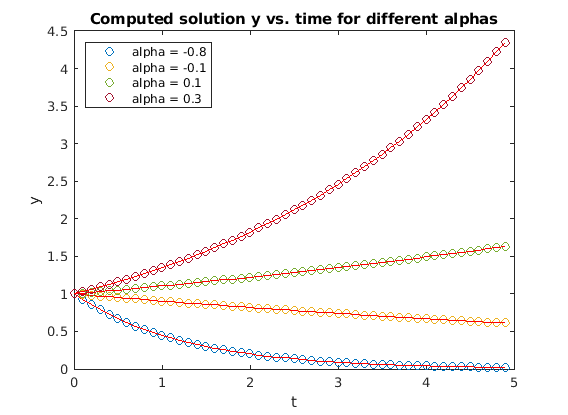
\includegraphics[width=0.7\columnwidth]{AdamsBashforth3Exponential.png}
	\caption{The exponential growth ODE integrated using 3rd order Adams-Bashforth.}
	\label{fig:AdamsBashforth3Exponential}
\end{figure}
\begin{figure}[tbh]
	\centering
	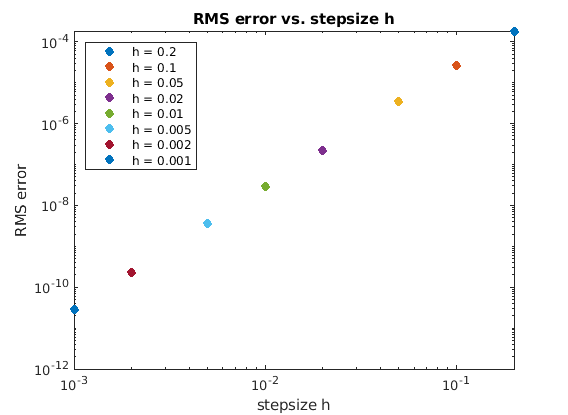
\includegraphics[width=0.7\columnwidth]{AdamsBashforth3ExponentialErr.png}
	\caption{Error scaling of 3rd order Adams-Bashforth.  The error scales as $O(h^3)$.}
	\label{fig:AdamsBashforth3ExponentialErr}
\end{figure}



\section{Adams-Moulton method -- 3nd order}
The Adams-Bashforth methods are explicit -- they use the value of $y$ at the present and past times to compute a the step into the future.  Multistep methods may also be implicit -- the trapezoidal method is an example of a implicit multistep method you have already see above.  Higher order implicit multistep methods also exist.  One class are the Adams-Molulton methods.  Like Adams-Bashforth, they use interpolation to fit a polynomial to the previous $f(t,y)$ values, but Adams-Moulton methods incorporate the future $y$ into the interpolation too.  The basic idea is shown in \cref{fig:AdamsMoulton3}.  
\begin{figure}[tbh]
	\centering
	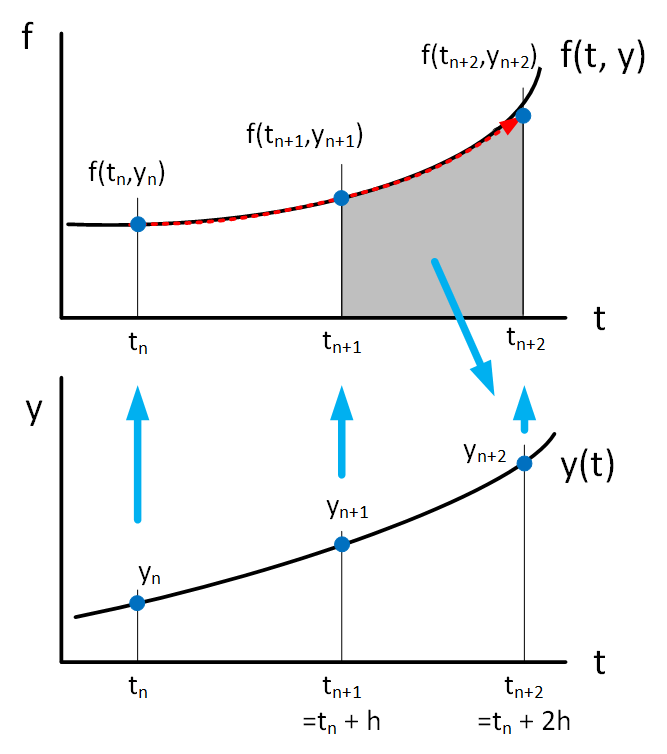
\includegraphics[width=0.7\columnwidth]{AdamsMoulton3.png}
	\caption{Third-order Adams-Moulton method.}
	\label{fig:AdamsMoulton3}
\end{figure}
The method interpolates the function $f(t,y)$ at the points $t_0$ (past), $t_1$ (present), and $t_2$ (future) using the Lagrange polynomial
\begin{gather}
f(t) = \frac{(t-t_{n+1})(t-t_{n+2})}{(t_{n}-t_{n+1})(t_{n}-t_{n+2})} f_{n}
+\frac{(t-t_{n})(t-t_{n+2})}{(t_{n+1}-t_{n})(t_{n+1}-t_{n+2})} f_{n+1} \\
\nonumber
+\frac{(t-t_{n})(t-t_{n+1})}{(t_{n+2}-t_{n})(t_{n+2}-t_{n+1})} f_{n+2}
\end{gather}
so the iteration is
\begin{equation}
\label{eq:AdamsMoultonInterpolation}
y_{n+2} = \int_{t_{n+2}}^{t_{n+3}} 
\frac{(t-t_{n+1})(t-t_{n+2})}{2 h^2} f_{n}
+\frac{(t-t_{n})(t-t_{n+2})}{-h^2} f_{n+1}
+\frac{(t-t_{n})(t-t_{n+1})}{2 h^2} f_{n+2}
dt 
+ y_{n+1}
\end{equation}
Note that $f_{n+2} = f(t_{n+2}, y_{n+2})$ so $y_{n+2}$ appears on both sides of \cref{eq:AdamsMoultonInterpolation} -- the method is implicit.  Nonetheless, we can treat it as a constant factor $f_{n+2}$ and go ahead and perform the integral.  Change variables as usual: $\alpha = (t-t_0)/h$ so $h d\alpha = dt$ and the integral becomes
\begin{equation}
\label{eq:AdamsMoultonIntegral}
y_{n+2} = h \int_1^2 
\frac{(\alpha-1)(\alpha-2)}{2} f_{n}
-\alpha(\alpha-2) f_{n+1}
+\frac{\alpha(\alpha-1)}{2} f_{n+2}
dt 
+ y_{n+1}
\end{equation}
Evaluating each term yields the third-order Adams-Moulton method:
\begin{equation}
\label{eq:AdamsMoultonIntegral1}
y_{n+2} = h \left( -\frac{1}{12} f_n + \frac{2}{3} f_{n+1} + \frac{5}{12} f_{n+2} \right)
+ y_{n+1}
\end{equation}
Again, since $f_{n+2} = f(t_{n+2}, y_{n+2})$, the equation \cref{eq:AdamsMoultonIntegral1} must be solved using a rootfinder to get $y_{n+2}$, but you should be comfortable with such implicit methods by now.


\section{Example: Adams methods and the Van der Pol oscillator}
Here is a quick demonstration showing why implicit methods like Adams-Moulton are useful, despite requiring a rootfinder.  
\begin{figure}[h!]
	\centering
	\includegraphics[width=0.6\columnwidth]{AdamsBashforth3VanderPol.png}
	\caption{Third-order Adams-Bashforth method solving the Van der Pol system.  Stepsizes $h = 0.1$ and $0.01$ were used.  The method is clearly unstable for $h = 0.1$ -- the y-axis of the graph bottoms out at -1e177, indicating that the solution has exploded!  The method is stable for $h = 0.01$ but is not as accurate as the Adams-Moulton method shown in \cref{fig:AdamsMoulton3VanderPol}.}
	\label{fig:AdamsBashforth3VanderPol}
\end{figure}
\begin{figure}[h!]
	\centering
	\includegraphics[width=0.6\columnwidth]{AdamsMoulton3VanderPol.png}
	\caption{Third-order Adams-Moulton method solving the Van der Pol system.  The stepsizes were $h = 0.1$ and $0.01$.  In contrast to the Adams-Bashforth result shown in \cref{fig:AdamsBashforth3VanderPol}, the Adam-Moulton method remains stable for $h = 0.1$.}
	\label{fig:AdamsMoulton3VanderPol}
\end{figure}
I have written programs implementing 3rd order Adams-Bashforth and 3rd order Adams-Moulton to integrate the Van der Pol oscillator \cref{eq:VanDerPolOsc}.  Recall that the Van der Pol system is stiff, and good practice recommends you use implicit methods when integrating stiff ODEs.  The reason is that implicit systems can use larger stepsizes without difficulty, so they can quickly solve a stiff system which would force an explicit method like Adams-Bashforth to use small steps.  

Shown in \cref{fig:AdamsBashforth3VanderPol} and \cref{fig:AdamsMoulton3VanderPol} are plots of the Van der Pol solution computed by 3rd order Adams-Bashforth (explicit) vs. 3rd order Adams-Moulton (implicit).  Both solvers used stepsize $h = 0.1$.  At first glance, the result of the Adams-Bashforth computation looks odd.  The reason is that the Adams-Bashforth method became unstable, so its output exploded to roughly $y = -1e177$ -- the method is useless for Van der Pol at this stepsize.  (Of course, you can decrease the stepsize at the cost of a longer simulation time.  That's not a problem for this toy problem, but if you are faced with a large computation which takes many hours, you want to squeeze as much performance out of your method as possible.)  On the other hand, Adams-Moulton works just fine at this stepsize.  

I should mention that there is a trade-off between these two methods:  Adams-Bashforth requires much smaller stepsize to handle the Van der Pol system, but Adams-Moulton runs a nonlinear solver (Matlab's fslove()) at each step.  Solvers are typically iterative, so they can take significant time to converge on a solution.  Therefore, Adams-Bashforth requires less computation per step, but is unstable unless the stepsize is small.  On the other hand, the Adams-Moulton method takes longer per step, but remains stable for larger stepsizes.  Which method to choose depends upon the particular details of your problem -- you typically need to experiment with different methods and different stepsizes to find the best way to solve your particular problem.


\section{Generalizations}
There is a whole family of linear multistep methods of orders 2, 3, 4, 5, 6, and so on.  The general pattern employed by these methods looks like this:
\begin{equation}
\label{eq:LMMGeneralOrder}
\alpha_0 y_i + \alpha_1 y_{i+1} + \alpha_2 y_{i+2} + \cdots + y_{i+k} =
h \left(\beta_0 f_i + \beta_1 f_{i+1}  + \beta_2 f_{i+2} + \cdots + \beta_{k} f_{i+k}  \right) 
\end{equation}
These are called $k$-step methods.  Some things to note:
\begin{itemize}
	\item The coefficient in front of the term $y_{i+k}$ on the LHS is one.  This is the future value which we wish to find.
	\item If we set all $\alpha_j = 0$ except $\alpha_{k-1}$ and additionally set $\beta_{k}=0$ then we recover the explicit Adams-Bashforth methods.
	\item If we set all $\alpha_j = 0$ except $\alpha_{k-1}$ and keep non-zero $\beta_{k}$ then we get the Adams-Moulton methods.
	\item I won't prove it here, but it can be shown that a $k$-step Adams-Bashforth method has order $O(h^k)$ while a $k$-step Adams-Moulton method has order $O(h^{k+1})$.  That's another advantage of the implicit over the explicit methods.
	\item Keeping additional $\alpha_j$ terms gives so-called backward difference methods.  Those methods are outside of the scope of this class.
	\item Regarding stability of linear multistep methods, there is a large body of well-developed theory specifying conditions under which they are stable.  That theory is also outside the scope of this class.
\end{itemize}
High-order linear multistep methods like these are implemented in high-end ODE solvers like the Sundials suite from Lawrence Livermore National Laboratories.  Most likely, in your work you will just call such a "canned" solver rather than writing your own, so you are spared the complexities of implementing such a solver.

% Example:  Rate equations.
% Example:  Chemical reactions.
% Example:  Epidemeological models.
% Example:  Chaos -- Roessler & Lorenz systems

\section{Chapter summary}
Here are the important points made in this chapter:
\begin{itemize}
	\item Linear multistep methods are derived by interpolating previously-computed (and sometimes future) points and using the interpolation in \cref{eq:integratedODE} to compute solution points in the future.
	\item The order of linear multistep methods is increased by incorporating more interpolation points into the interpolated approximation for $f(t, y)$.  We examined the trapezoid (1st order), Adams-Bashforth (2nd and 3rd order), and Adams-Moulton (3rd order) methods.
	\item Adams-Bashforth methods are explicit, Adams-Moulton are implicit.   
	\item Implicit methods like Adam-Moulton are recommended for stiff systems since they remain stable while also allowing for larger steps than explicit methods.  However, implicit methods require running a rootfinder at every step, so a performance trade-off exists between explicit and implicit methods.
	\item The methods examined in this chapter are members of a large class of linear multistep methods described by \cref{eq:LMMGeneralOrder}.  Such methods are commonly provided in high-end ODE solvers.  
\end{itemize}


\chapter{Symplectic integrators}
\label{sect:SymplecticIntegrators}

\section{Energy conserving ODEs}
\label{sect:EnergyConservation}
The ODE solvers examined thus far are meant for general purpose applications.   However, these is a special set of ODEs which are not well served by the general purpose methods.  Those are ODEs which describe mechanical systems undergoing lossless motion.  "Lossless" means the system does not dissipate energy. Some examples are:
\begin{itemize}
	\item The frictionless simple harmonic oscillator, which we have seen many times already.
	\item The frictionless hanging pendulum.
	\item Motion of planets or satellites in space.
\end{itemize}
You might regard the first two examples as oversimple models.  However, a pendulum swinging in a vacuum is very close to lossless.  The LIGO apparatus which detected gravitational waves used pendulums hanging in a vacuum as part of its operation, so the (almost) frictionless pendulum is a physical reality.  Also, the motion of objects in space occurs with almost no dissipation -- there is no atmosphere to provide resistance to motion.  Accurately simulating their motion requires ODE solvers which respect the fact they experience no friction when moving -- they don't dissipate any energy.  Unfortunately, the problem with ODE solvers studied so far is that none of them conserve energy.  If you want to calculate the trajectory a rocket must travel in order to dock with the orbiting space station, it's crucial that your ODE solver calculates the trajectory perfectly, and that means it needs compute trajectories which are energy conserving.

What is energy?  In a physics class you probably learned that energy is something which is conserved.  But what does that mean?  And why is kinetic energy $(1/2) m v^2$?  What is going on, mathematically?  

For some insights we once again turn to the simple harmonic oscillator,
\begin{equation}
\label{eq:SHO2}
m \frac{d^2 y}{d t^2} = -k y
\end{equation}
Associated with this equation is a so-called energy,
\begin{equation}
\label{eq:SHOEnergy}
E = \frac{1}{2} m \left( \frac{d y}{d t} \right)^2 + \frac{1}{2} k y^2 
\end{equation}
which is a function of the variables position $y$ and velocity $dy/dt$.  From your physics class you may recognize the term on the left as the "kinetic energy" and the term on the right as the "potential energy" of the SHO.  The important property of this energy definition is that any solution $y(t)$ of the ODE \cref{eq:SHO2} will automatically conserve the energy function \cref{eq:SHOEnergy}.  "Conserve" means that the energy $E$ will remain constant for all times.  This can be shown by considering the time derivative of $E$. 
\begin{equation}
\frac{d E}{d t} = m \left( \frac{d y}{d t} \right)\left( \frac{d^2 y}{d t^2} \right) + k y \left( \frac{d y}{d t} \right)
\end{equation}
then substitute the value of $m (d^2 y/d t^2)$ from \cref{eq:SHO2} into this equation to get
\begin{align}
\frac{d E}{d t} =& -k y \left( \frac{d y}{d t} \right) + k y \left( \frac{d y}{d t} \right) \\
=& 0
\end{align}
This says that $E$ never changes -- it is conserved by any solution to \cref{eq:SHO2}.  In general, some -- but not all -- ODEs admit an energy which is conserved.  The exact form of the energy depends upon the ODE under consideration.  But if a conserved energy exists for a particular ODE, then a good solver should produce solutions which conserve energy.  Unfortunately, most solvers don't.  We have seen this several times through the course of this booklet -- see \cref{fig:ForwardEulerSHOPropagator}, \cref{fig:BackwardEulerSHOPropagator}, \cref{fig:HeunsMethodSHODiff}, and \cref{fig:RK4SHODiff}.  Those figures all show the amplitude of the oscillation growing or shrinking with increasing time -- behavior which evidences the energy is changing with time.

There is a class of solvers which do conserve energy.  They fall under the rubric "symplectic integrators".  The reason they have this name has to do with Hamiltonian mechanics, a generalization of Newtonian mechanics which we will touch on in \cref{sect:PhaseSpaceConservation}.  Symplectic integrators are used only for second-degree ODEs such as found in Newton's second law.  Consequently, they are very important for calculating the motion of objects in space, including planets, spacecraft, comets, and so on.  They come in many orders of accuracy, similar to the other solvers discussed in this booklet.  I will only discuss the simplest method -- symplectic Euler -- here since this symplectic integrators are a specialized subject and it's enough to simply see the concepts rather than review the entire field.

\section{Symplectic Euler}
As mentioned above, symplectic integrators are used to solve second-degree ODEs.l  That means the integrators are applied to a system of two 1st-degree ODEs.  That is, we start with teh system to solve
\begin{equation}
\begin{aligned}
\frac{d u}{d t} =& f(t, v) \\
\frac{d v}{d t} =& g(t, u)
\end{aligned}
\label{eq:SymplecticODE}
\end{equation}
With this definition, here is symplectic Euler:
\begin{equation}
\begin{aligned}
v_{n+1} =& v_n + h g(t_n, u_n) \\
u_{n+1} =& u_n + h f(t_n, v_{n+1})
\end{aligned}
\label{eq:SymplecticEuler}
\end{equation}
Note that first $v$ is updated, then $u$ us updated using the already updated $v$.  The method is symmetric with respect to which is updated first,, so you can also use
\begin{equation}
\begin{aligned}
u_{n+1} =& u_n + h f(t_n, v_{n})
v_{n+1} =& v_n + h g(t_n, u_n+1) \\
\end{aligned}
\label{eq:SymplecticEuler}
\end{equation}
This is sometimes called a semi-implicit method (or semi-implicit Euler scheme) since the updated value $v_{n+1}$ (or $u_{n+1}$)is used in the middle of the full two-step computation.


\section{Example: the simple harmonic oscillator}
We know the analytical solutions of the simple harmonic oscillator equation \cref{eq:SHO2} conserve energy.  Now we will see if the solution produced by symplectic Euler also conserves energy.  For the RHS of \cref{eq:SymplecticODE} we have
\begin{align}
\nonumber
f(t, v)  =& -\omega^2 v \\
\nonumber
g(t, u)  =& u
\end{align}
using the usual definition $\omega^2 = k/m$.  Inserting these into \cref{eq:SymplecticEuler} yields
\begin{equation}
\begin{aligned}
v_{n+1} =& v_n + h u_n \\
u_{n+1} =& u_n - h \omega^2 v_{n+1}
\end{aligned}
\label{eq:SymplecticEulerSHO}
\end{equation}
We could implement this system on the computer as it stands, but for the purposes of stability analysis we will convert it into a matrix propagator form.  To do so move the future to the LHS and the present to the RHS.  We get
\begin{equation}
\nonumber
\begin{aligned}
u_{n+1} + h \omega^2 v_{n+1}  =& u_n \\
v_{n+1} =& v_n + h u_n 
\end{aligned}
\end{equation}

Now write both sides as matrix-vector products.  We get
\begin{equation}
\nonumber
\begin{pmatrix}
1 &  h \omega^2 \\
0 & 1
\end{pmatrix}
\begin{pmatrix}
u_{n+1} \\
v_{n+1}
\end{pmatrix}
=
\begin{pmatrix}
1 &  0 \\
h & 1
\end{pmatrix}
\begin{pmatrix}
u_{n} \\
v_{n}
\end{pmatrix}
\end{equation}
Now move the LHS matrix to the RHS
\begin{equation}
\nonumber
\begin{pmatrix}
u_{n+1} \\
v_{n+1}
\end{pmatrix}
=
\begin{pmatrix}
1 &  h \omega^2 \\
0 & 1
\end{pmatrix}^{-1}
\begin{pmatrix}
1 &  0 \\
h & 1
\end{pmatrix}
\begin{pmatrix}
u_{n} \\
v_{n}
\end{pmatrix}
\end{equation}
Simplifying, this becomes
\begin{equation}
\begin{pmatrix}
u_{n+1} \\
v_{n+1}
\end{pmatrix}
=
\begin{pmatrix}
1 - h^2 \omega^2&  -h \omega^2 \\
h & 1
\end{pmatrix}
\begin{pmatrix}
u_{n} \\
v_{n}
\end{pmatrix}
\end{equation}
\begin{figure}[ht]
	\centering
	\includegraphics[width=0.7\columnwidth]{SymplecticEulerSHO.png}
	\caption{The simple harmonic oscillator integrated using symplectic Euler.  Note the longer time span than plotted for previous solutions of the SHO.  No growth nor decay of the oscillation is evident in this plot -- the energy of the solution is conserved by the method, at least at this scale.  }
	\label{fig:SymplecticEulerSHO}
\end{figure}
This defines an iteration method using the matrix as a propagator.  Note the similarity to the forward Euler propagation matrix \cref{eq:SHOMatVecSystem}:  only the (1,1) element is different.  
The results of implementing this iteration are shown in \cref{fig:SymplecticEulerSHO}.  Unlike the cases of forward and backward Euler, this method evidences no growth nor decay of the oscillation amplitude with time.
Energy conservation is also shown in \cref{fig:SymplecticEulerEnergy} which plots $u(t)^2 + \omega^2 v(t)^2$.  In analogy to $\sin^2(t) + cos^2(t) = 1$, the energy $u(t)^2 + \omega^2 v(t)^2$ should remain constant.  It does, except it evinces little wiggles which depend upon time.  Note that the average value remains equal to one.
\begin{figure}[htb]
	\centering
	\includegraphics[width=0.7\columnwidth]{SymplecticEulerEnergy.png}
	\caption{A plot of $u(t)^2 + \omega^2 v(t)^2$ which shows symplectic Euler conserves energy on average.  Note that the amplitude remains close to one over the entire simulation time.  It wiggles up and down but does not grow nor shrink over a longer time scale.}
	\label{fig:SymplecticEulerEnergy}
\end{figure}

Of course, now the question is why does symplectic Euler conserve energy?  As usual, the answer lies in computing the eigenvalues of the propagator matrix.  Call $g$ the eigenvalue (again, for "growth factor").  The eigenvalue equation is then
\begin{equation}
\nonumber
	det
\begin{pmatrix}
	1 - h^2 \omega^2  - g  &  -h \omega^2 \\
	h & 1 - g
\end{pmatrix}
= 0
\end{equation}
Solving for $g$ gives
\begin{equation}
\label{eq:SymplecticEulerSHOGrowthFactor}
g = 1 - \frac{h^2 \omega^2}{2} \pm \frac{h \omega  \sqrt{h^2 \omega^2 - 4}}{2}
\end{equation}
This is a nasty expression at first glance.  However, our goal is to see if $|g| = 1$ for any values of $h \omega$.  If $|g| = 1$ then we have a method which does not cause the solution amplitude to grow or decay.  Therefore, an easy way to understand \cref{eq:SymplecticEulerSHOGrowthFactor} is to simply use Matlab to plot $|g|$ vs. $h \omega$.  This is shown in \cref{fig:SymplecticEulerGFactor}.  We see that $|g| = 1$ when $|h \omega| < 2$.  Therefore, symplectic Euler method maintains the amplitude of the simple harmonic oscillator -- that is, it conserves energy.  
\begin{figure}[h]
	\centering
	\includegraphics[width=0.7\columnwidth]{SymplecticEulerGFactor.png}
	\caption{The growth factor $|g|$ plotted vs. $h \omega$.  The growth factor is exactly one when $|h \omega| < 2$.  Therefore, in this range the symplectic Euler method maintains the amplitude of the simple harmonic oscillator -- that is, it conserves energy.  However, the plots walk away from each other in time depending upon the value of $h$.}
	\label{fig:SymplecticEulerGFactor}
\end{figure}

Knowing that $|g| = 1$ when $|h \omega| < 2$ allows us to take a few additional easy analytic steps.  When $|h \omega| < 2$ the rightmost term in \cref{eq:SymplecticEulerSHOGrowthFactor} is pure imaginary while the other two terms are real.  That means we can compute $|g|^2 = \Re(g)^2 + \Im(g)^2$,
\begin{equation}
\nonumber
|g|^2 = \left(1 - \frac{h^2 \omega^2}{2}\right)^2 + \left( \frac{h \omega  \sqrt{4 - h^2 \omega^2}}{2} \right)^2
\end{equation}
\begin{equation}
\nonumber
= \left(1 - h^2 \omega^2 + \left( \frac{h^2 \omega^2}{2} \right)^2 \right) + \left( \frac{h^2 \omega^2  (4 - h^2 \omega^2)}{4} \right)
\end{equation}
\begin{equation}
\nonumber
= 1
\end{equation}
as was found in the plot \cref{fig:SymplecticEulerGFactor}.  This confirms our numerical observation in \cref{fig:SymplecticEulerGFactor} that $|g| = 1$.  Outside this range, the growth factor is not one, meaning that symplectic Euler doesn't conserve energy outside of the range 
$|h \omega| < 2$.  However, this is not a big limitation since one generally needs $h \ll 1/\omega$ to compute smooth oscillations.  That is, you need to sample at least a couple of points inside each oscillation in order to simulate it accurately, so achieving $|h \omega| < 2$ is compatible with choosing a good step size.

\section{Conservative systems, phase space, and Liouville's theorem}
\label{sect:PhaseSpaceConservation}
This section is a brief detour into the physics of energy conservation in classical mechanics.  At the beginning of \cref{sect:SymplecticIntegrators} above I mentioned that some, but not all ODEs have an accompanying energy.  In advanced mechanics, the equations of motion of a system which conserves energy are found by first writing down a so-called "Hamiltonian", and then deriving the position and momentum of all particles in the system from the Hamiltonian.  The Hamiltonian is a scalar function which plays the role of the energy of the system, but is written in terms of position and momentum variables.  For the SHO, the Hamiltonian is
\begin{equation}
\label{eq:SHOHamiltonian}
H(p,x) = \frac{p^2}{2 m} + \frac{1}{2} k x^2
\end{equation}
where $p$ is the momentum of the oscillator and $x$ is its position.  Note this is the same as the total energy \cref{eq:SHOEnergy} where we have replaced the kinetic energy written in terms of the velocity $m v^2 / 2$ with the equivalent expression written in terms of momentum, $p^2/2 m$.  Then, to get the equations of motion of the system, the Hamiltonian formalism says they are found from Hamilton's equations,
\begin{equation}
\frac{d x}{d t} = \frac{\partial H}{ \partial p} 
\end{equation}
\begin{equation}
\frac{d p}{d t} = -\frac{\partial H}{ \partial x} 
\end{equation}
In the case of the SHO we use the Hamiltonian \cref{eq:SHOHamiltonian} and these equations to get the equations of motion of the oscillator,
\begin{equation}
\nonumber
\frac{d x}{d t} = \frac{p}{m} 
\end{equation}
\begin{equation}
\nonumber
\frac{d p}{d t} = -k x
\end{equation}
This pair of equations should remind you strongly of those introduced back in \cref{SHOSystem} -- they're the same equations but written in terms of position and momentum instead of position and velocity.  In Hamiltonian mechanics, you first use physical reasoning to construct and write down a Hamiltonian.  Then you derive the equations of motion from the Hamiltonian using these equations.  The point is that Hamiltonian mechanics gives you a general, step-by-step procedure to derive the equations of motion of any system.  By contrast, Newtonian mechanics relies on ad-hoc arguments about forces and accelerations to derive the equations of motion, and every system is handled differently depending upon its physical configuration.

Since the Hamiltonian is the energy function of the system, it is conserved as long as time does not appear explicitly in its formula.  This is clearly the case for the SHO Hamiltonian, \cref{eq:SHOHamiltonian}.  At a deep level, energy conservation is a consequence of Noether's theorem, which says that every symmetry of the Hamiltonian implies a corresponding conserved quantity.  For the SHO Hamiltonian, we may replace time $t$ with $t + \tau$, where $\tau$ represents a constant shift of the time axis.  Upon making this replacement  $t \rightarrow t + \tau$, the form of the Hamiltonian remains the same.  That is, this Hamiltonian is invariant with respect to the transformation $t \rightarrow t + \tau$.  Another way to say it is that the Hamiltonian is symmetric with respect to time shifts.  As a consequence of Noether's theorem, this symmetry implies an associated quantity is conserved, and in this case the conserved quantity is the energy.  This should answer the question posed back in \cref{sect:EnergyConservation}, why is energy conserved for the SHO?  Energy is conserved by the SHO because its Hamiltonian has time-shift symmetry!  Noether's theorem is very profound and is used by physicists to reason about many different conserved quantities like electric charge, mass, parity, and other quantities.  Unfortunately, while it is very interesting, further discussion of Noether's theorem is far outside the scope of this booklet.

Another important result from classical mechanics is that any system derived from a time-invariant Hamiltonian will conserve volumes in phase space.  What does this mean?  
\begin{itemize}
	\item First, phase space is defined as the space of all possible states of the system.  For example, a body undergoing one-dimensional motion has a two-dimensional phase space: the set of all possible positions and momenta, $[x, p]$ without regard for any equations of motion.  (Equations of motion will be imposed later and will naturally restrict the set of possible $[x, p]$ to orbits within the full phase space.)
	\item Once the phase space is defined, any particular mechanical system may be described via a Hamiltonian defined on the phase space.  Different mechanical systems will be described by different Hamiltonians.  For example, the SHO has Hamiltonian $H = p^2/2m + k x^2/2$ while the hanging pendulum has Hamiltonian $H = p^2/2m + m g \cos(\theta)/2$.
	\item A time-invariant Hamiltonian is one which has no explicit dependence on time -- the variable $t$ does not appear in its formula.  This is obviously the case for the SHO Hamiltonian \cref{eq:SHOHamiltonian}.
	\item The equations of motion derived from the Hamiltonian will define how any particular point $[x(t),p(t)]$ will evolve in time.  You can visualize the evolution of a single point as a trajectory moving through phase space.
	\item Next consider a small region of phase space surrounding the initial phase-space point $[x(0),p(0)]$.  See \cref{fig:PhaseSpaceVolumes}.  Now ask, what happens to the volume of the region as time moves forward.  Louiville's theorem says that the volume $V$ remains constant as the system evolves.  That is, the blue region shown in the figure may twist and deform, but its volume will remain the same for all time.
\end{itemize}
\begin{figure}[ht]
	\centering
	\includegraphics[width=0.7\columnwidth]{PhaseSpaceVolumes.png}
	\caption{Liouville's theorem says that phase space volumes remain the same size when the system evolves under the action of a (time invariant) Hamiltonian.}
	\label{fig:PhaseSpaceVolumes}
\end{figure}
A general proof of Liouville's theorem is more difficult than I can explain in this booklet.  But I will demonstrate that $[p(t), x(t)]^T$ trajectories generated by the SHO Hamiltonian conserve phase space volumes, and you can use my demonstration as motivation for accepting the general theorem.

Before examining the SHO, I want to start by considering what it means to measure volumes in phase space.  I also give a criterion for recognizing when volume is conserved under a transformation.  I will use a very simple picture to convey these ideas.  Consider the case of a small square in a two-dimensional phase space.  Take the sides of the square to be defined by two vectors, $u$ and $v$.  Now consider what happens to $u$ and $v$ under a linear transform.  "Linear transform" means matrix-vector multiplication.  Under action of a $2 \times 2$ matrix $T$, we have
\begin{equation}
\label{eq:LinearTransform}
\begin{pmatrix}
 u' \\
 v'
\end{pmatrix}
=
T
\begin{pmatrix}
 u \\
 v
\end{pmatrix}
\end{equation}
We think of $[u', v']^T$ as the output of the transformation, and $T$ is the thing doing the transformation.

In your previous linear algebra class you probably learned that applying a linear transform to a vector produced a stretched and rotated copy of the input vector.  If you're lucky you may have seen that applying a linear transform to a square (whose sides are defined by two vectors) produced a parallelpiped output.  This is shown in 
\cref{fig:LinearTransform}. 
\begin{figure}[ht]
	\centering
	\includegraphics[width=0.5\columnwidth]{LinearTransform.png}
	\caption{The action of the linear transform (matrix) $T$ on vectors $u$ and $v$.  In each case, the transformed result $T u$ and $T v$ is a stretched and rotated copy of the original vector.  The initial square formed by $u$ and $v$ is thereby transformed into a parallelpiped.}
	\label{fig:LinearTransform}
\end{figure}
Now how to compute the volume (or area when working in 2D) of these shapes?  Recall that the area subtended by the two vectors may be found using the determinant formula,
\begin{equation}
\label{eq:AreaDeterminant}
\begin{aligned}
A &= 
\begin{vmatrix}
u_1 & u_2 \\
v_1 & v_2
\end{vmatrix} \\
&= u_1 v_2 - u_2 v_1
\end{aligned}
\end{equation}
where we use the components of the vectors, $u = [u_1, u_2]^T$ and $v = [v_1, v_2]^T$.  Another way to write this is using  a quadratic form
\begin{equation}
\label{eq:SymplecticForm}
A = 
\begin{pmatrix}
u_1 & u_2 \\
\end{pmatrix}
\begin{pmatrix}
0 & 1 \\
-1 & 0
\end{pmatrix}
\begin{pmatrix}
v_1 \\ v_2
\end{pmatrix}
= u_1 v_2 - u_2 v_1
\end{equation}
You can easily see \cref{eq:AreaDeterminant} and \cref{eq:SymplecticForm} give the same result by inspection.  Due to its importance, we will give the matrix the name $J$, so
\begin{equation}
\nonumber
J = 
\begin{pmatrix}
0 & 1 \\
-1 & 0
\end{pmatrix} \\
\end{equation}

Now consider what it means for a transformation $T$ to preserve volume.  To preserve area we require that input area equals output area,
\begin{align}
\nonumber
u^T J v &= u'^T J v' \\
\nonumber
&= u^T T^T J T v
\end{align}
or we can drop the $u$ and $v$ and focus on the transformation itself.  This equation requires the transformation obey
\begin{equation}
\label{eq:SymplecticDef}
J = T^T J T
\end{equation}
A linear transform (matrix) which obeys \cref{eq:SymplecticDef} is called "symplectic".  If a transform $T$ is symplectic, that means it preserves volumes.

We just looked at a symplectic linear transform.  But what about the case of a general transform?  And what does this have to do with Hamiltonians, energy conservation, and ODEs?  Let's again write down the SHO Hamiltonian, this time in non-dimensional form.  (I don't want to try to explain away the mass and stiffness constants in the below discussion -- they would only make matters complicated.)  The Hamiltonian is
\begin{equation}
\label{eq:NonDimensionalSHOHamiltonian}
H = \frac{1}{2}p^2 + \frac{1}{2} x^2
\end{equation}
Because time does not appear explicitly in this Hamiltonian, the system it describes will conserve energy.  Now consider the motion of a point $[p, x]^T$ in the phase space governed by this Hamiltonian.  The equations of motion obeyed by the point are
\begin{equation}
\label{eq:FirstPoint}
\frac{d}{dt}
\begin{pmatrix}
p \\
x
\end{pmatrix}
 = 
\begin{pmatrix}
-\partial H / \partial x \\
\partial H / \partial p
\end{pmatrix}
\end{equation}
Next consider the trajectory of a point displaced from $[p, x]^T$ by $[\Delta p, \Delta x]^T$.  We imagine these are the sides of the little volume we want to track.  The displaced point's motion is given by
\begin{equation}
\nonumber
\frac{d}{dt}
\begin{pmatrix}
p + \Delta p \\
x + \Delta x
\end{pmatrix}
= 
\begin{pmatrix}
-\partial H / \partial x \\
\partial H / \partial p
\end{pmatrix}
\end{equation}
Assuming $[\Delta p, \Delta x]^T$ are both small, we can approximate the motion using a Taylor series expansion,
\begin{equation}
\label{eq:SecondPoint}
\frac{d}{dt}
\begin{pmatrix}
p + \Delta p \\
x + \Delta x
\end{pmatrix}
\approx
\left.
\begin{pmatrix}
-\partial H / \partial x \\
\partial H / \partial p
\end{pmatrix}
\right|_{p,x}
+
\left.
\begin{pmatrix}
-\partial^2 H / \partial x \partial p \\
\partial^2 H / \partial p^2
\end{pmatrix}
\right|_{p,x}
\Delta p
+
\left.
\begin{pmatrix}
-\partial^2 H / \partial x^2 \\
\partial^2 H / \partial p \partial x
\end{pmatrix}
\right|_{p,x}
\Delta x
\end{equation}
Now subtract \cref{eq:FirstPoint} from \cref{eq:SecondPoint}, and use the common notation for partial derivatives to get an expression for the evolution of the sides of the little volume,
\begin{equation}
\nonumber
\frac{d}{dt}
\begin{pmatrix}
\Delta p \\
\Delta x
\end{pmatrix}
\approx
\left.
\begin{pmatrix}
-H_{xp} & -H_{xx} \\
H_{pp} & H_{px}
\end{pmatrix}
\right|_{p,x}
\begin{pmatrix}
\Delta p \\
\Delta x
\end{pmatrix}
\end{equation}
This equation says that the change in the sides of the initial square is driven by the matrix of partial derivatives.  That is, the partial derivative matrix plays the role of the transformation matrix $A$ in \cref{eq:SymplecticForm}.  Therefore, we can say that the volume of the square remains constant under evolution if the symplicity condition \cref{eq:SymplecticDef} holds.  That is, to conserve phase space volumes, we want the following condition to hold for the SHO Hamiltonian:
\begin{equation}
\label{eq:SHOConservePhaseSpaceVols}
\begin{pmatrix}
0 & 1 \\
-1 & 0
\end{pmatrix}
=
\begin{pmatrix}
-H_{xp} & H_{pp} \\
-H_{xx} & H_{px}
\end{pmatrix}
\begin{pmatrix}
0 & 1 \\
-1 & 0
\end{pmatrix}
\begin{pmatrix}
-H_{xp} & -H_{xx} \\
H_{pp} & H_{px}
\end{pmatrix}
\end{equation}
For the SHO Hamiltonian we have
\begin{align}
\nonumber
H_{xx} &= \frac{\partial^2 H}{\partial x^2} = 1 \\
\nonumber
H_{pp} &= \frac{\partial^2 H}{\partial p^2} = 1 \\
\nonumber
H_{xp} &= H_{px} = 0
\end{align}
Upon inserting these values into \cref{eq:SHOConservePhaseSpaceVols} and evaluating, we get
\begin{align}
\nonumber
&\phantom{=i}
\begin{pmatrix}
0 & 1 \\
-1 & 0
\end{pmatrix}
\begin{pmatrix}
0 & 1 \\
-1 & 0
\end{pmatrix}
\begin{pmatrix}
0 & -1 \\
1 & 0
\end{pmatrix} \\
\nonumber
&=
\begin{pmatrix}
0 & 1 \\
-1 & 0
\end{pmatrix}
\begin{pmatrix}
1 & 0 \\
0 & 1
\end{pmatrix} \\
\nonumber
&=
\begin{pmatrix}
0 & 1 \\
-1 & 0
\end{pmatrix} \\
\nonumber
&= J
\end{align}
Therefore, the transformation matrix induced by the SHO Hamiltonian is symplectic.  And since it is symplectic, the transformation \cref{eq:SecondPoint} will preserve phase space volumes as promised.


\section{Euler methods and conservation of phase space volumes}
We end this booklet by looking at forward Euler and symplectic Euler and asking if one or both conserve phase space volumes.  I wrote Matlab programs which draw a rectangle in phase space, then evolve the points in the rectangle using forward Euler and symplectic Euler for four oscillation periods.  
\begin{figure}[h!]
\begin{subfigure}[t]{0.5\columnwidth}
	\centering
	\includegraphics[width=1.1\linewidth]{ForwardEulerPhaseSpace_ZoomOut.png}
	\caption{Forward Euler -- zoomed out.  The area under study starts as the rectangle at the 12 o'clock (top) of the circle.  Four oscillation periods later, the rectangle has obviously grown in size -- phase space area is not conserved.}
	\label{fig:ForwardEulerPhaseSpace_ZoomOut}
\end{subfigure}
\begin{subfigure}[t]{0.5\columnwidth}
	\centering
	\includegraphics[width=1.1\linewidth]{ForwardEulerPhaseSpace_ZoomIn.png}
	\caption{Forward Euler -- zoomed in.}
	\label{fig:ForwardEulerPhaseSpace_ZoomIn}
\end{subfigure}
\caption{Phase space volumes evolved by forward Euler.}
\label{fig:ForwardEulerPhaseSpace}
\end{figure}
\begin{figure}[t!]
	\begin{subfigure}[t]{0.5\columnwidth}
		\centering
		\includegraphics[width=1.1\linewidth]{SymplecticEulerPhaseSpace_ZoomOut.png}
		\caption{Symplectic Euler -- zoomed out. The area under study starts as the rectangle at the 12 o'clock (top) of the circle.  Four oscillation periods later the rectangle has not grown in size, nor has it left the circle.  The method is both stable and energy conserving. }
		\label{fig:SymplecticEulerPhaseSpace_ZoomOut}
	\end{subfigure}
	\begin{subfigure}[t]{0.5\columnwidth}
		\centering
		\includegraphics[width=1.1\linewidth]{SymplecticEulerPhaseSpace_ZoomIn.png}
		\caption{Symplectic Euler -- zoomed in.}
		\label{fig:SymplecticEulerPhaseSpace_ZoomIn}
	\end{subfigure}
	\caption{Phase space volumes evolved by symplectic Euler.}
	\label{fig:SymplecticEulerPhaseSpace}
\end{figure}
The program takes a snapshot of the rectangle multiple times during its evolution, and plots the rectanges on the circle of constant energy.  The simulation results are shown in \cref{fig:ForwardEulerPhaseSpace} and \cref{fig:SymplecticEulerPhaseSpace}.  The results are clear: for the SHO, forward Euler is neither stable, nor does it conserve phase space volumes.   However, symplectic Euler is both stable and also conserves phase space volumes as evidenced by the two plots.
\section{Chapter summary}
Here are the important points made in this chapter:
\begin{itemize}
	\item General purpose ODE integrators usually don't conserve energy.  Therefore, they are inappropriate for problems where energy conservation is important, such as simulation of motion in space.
	\item Symplectic integrators are specialty solvers used for exactly those situations where it's important that the ODE solver ensure conservation of energy.  They are particularly common in computing the trajectories of objects in space.
	\item Energy conservation in mechanical systems is best understood in the context of Hamiltonian mechanics, which is a generalization of the Newtonian mechanics you probably learned about in your introductory physics classes.  
	\item Besides conserving energy, a symplectic system also conserves phase space volumes.  This fact is known as "Liouville's theorem".  A symplectic integrator will conserve phase space volumes as we demonstrated for the SHO -- both via analytic methods as well as simulation using the symplectic Euler method.
\end{itemize}
\chapter{Review and summary}
% Put a big table in here.  Table headings:  Method name, iteration, features/when to use, remarks.
Here are the important ideas discussed and points made in this booklet.
\begin{itemize}
	\item Many different ODE solvers of varying complexity and accuracy were presented.  A summary table of the methods is shown in \cref{tab:ODESolverOverview}.
	\item ODE solvers are broadly split into two categories:  explicit and implicit methods.  Explicit methods are those where the step forward in time (i.e. the future) may be calculated using the known values of the function $y$ (i.e. the present and the past).  Implicit methods are those where the step forward in time is calculated using the past, present and future simultaneously.  Implicit methods require running a rootfinder to make a step, explicit methods do not.
	\item Different ODE solvers have different levels of accuracy.  The accuracy of a particular method depends upon the stepsize $h$.  Typically, a solver provides more accurate solutions for smaller $h$, but at the expense of increased runtime.  The scaling of solver error usually behaves as $O(h^p)$ where $p$ is the "order" of the solver.  Higher $p$ implies better accuracy.
	\item A different way to categorize ODE solvers is one-step vs. multistep methods.  One-step methods take a step to $t_{n+1}$ based on information available only at time $t_n$ (and possibly some trial intermediate points).  The Runge-Kutta methods are examples of one-step methods.  Multistep methods take a step based on information from previous times $t_n$, $t_{n-1}$, $t_{n-2}$, etc.  The Adams-Bashforth methods are examples of explicit linear multistep methods, and Adams-Moulton methods are implicit multistep methods.
	\item The stability of a method refers whether a perturbation grows or shrinks as $t \rightarrow \infty$.   Different methods have different "stability domains", which are plots made by assuming $h$ is complex.  The plot shows what regions of the complex plane correspond to stability or instability.
	\item Adaptive step size methods make an estimate of the error incurred at each step, and adjust the stepsize up or down to maintain a given error tolerance.  Matlab's ode45 is a famous adaptive step size solver.  It is based on the Dormund-Prince 4/5 algorithm, a member of the Runge-Kutta family.
	\item Symplectic integrators are a subset of ODE solvers used in situations where the ODE is known to conserve energy.
\end{itemize}
\begin{table}[h]
\begin{center}
\renewcommand{\arraystretch}{1.5}
%\setlength\extrarowheight{2pt}
\begin{tabular}{ | p{3cm} | p{2cm} | p{2cm} | p{6cm} | } 
\hline
\textbf{Name} & \textbf{Type} & \textbf{Accuracy}  & \textbf{Iteration} \\
\hline
Forward Euler & Explicit & $O(h)$ & $y_{n+1} = y_n + h f(t_n, y_n)$  \\
\hline
Backward Euler & Implicit & $O(h)$  & $y_{n+1} = y_n + h f(t_{n+1}, y_{n+1})$ \\
\hline
Heun's method & Explicit, one-step & $O(h^2)$ & 
$\begin{aligned} 
s_1 &= h f(t_n, y_n) \\
\tilde{y} &= y_n + s_1 \\  
s_2 &=  h f(t_n, \tilde{y}) \\
y_{n+1} &= y_n + (h/2)(s_1 + s_2) 
\end{aligned}$  \\
\hline
Midpoint rule & Explicit, one-step & $O(h^2)$ & 
$\begin{aligned} 
k_1 &= h f(t_n, y_n) \\
k_2 &= h f(t_n+h/2, y_n + k_1/2) \\
y_{n+1} &= y_n + k_2
\end{aligned}$ \\
\hline
Fourth-order Runge-Kuttal & Explicit, one-step & $O(h^4)$ & 
$\begin{aligned}
k_1 &= h f(t_n, y_n) \\
k_2 &= h f(t_n+h/2, y_n + k_1/2) \\
k_3 &= h f(t_n+h/2, y_n + k_2/2) \\
k_4 &= h f(t_n+h, y_n + k_3) \\
y_{n+1} &= y_n + (k_1 + 2 k_2 + 2 k_3 + k_4)/6
\end{aligned}$ \\
\hline
Trapezoidal rule & Implicit & $O(h^2)$ & $y_{n+1} = \frac{h}{2} \left( f_{n+1} + f_n \right) + y_n$ \\
\hline
Second-order Adams-Bashforth & Explicit, multistep & $O(h^2)$ & 
$ y_{n+2} = h \left( \frac{3}{2} f_{n+1} - \frac{1}{2} f_{n} \right)   + y_{n+1}
$
\\
\hline
Third-order Adams-Bashforth & Explicit, multistep & $O(h^3)$ & 
$\begin{aligned}
y_{n+3} = & h \left(
\frac{5}{12} f_{n}
-\frac{4}{3} f_{n+1}
+\frac{23}{12} f_{n+2} \right) \\
& + y_{n+2}
\end{aligned}$
\\
\hline
Third-order Adams-Moulton & Implicit, multistep & $O(h^4)$ & 
$\begin{aligned}
y_{n+2} = & h \left( -\frac{1}{12} f_n + \frac{2}{3} f_{n+1}  + \frac{5}{12} f_{n+2} \right) \\
& + y_{n+1}
\end{aligned}$
\\
\hline
Symplectic Euler & Semi-implicit, 2nd order ODEs & $O(h)$ & 
$\begin{aligned}
	v_{n+1} &= v_n + h g(t_n, u_n) \\
	u_{n+1} &= u_n + h f(t_n, v_{n+1})
\end{aligned}$ \\
\hline
\end{tabular}
\caption{ODE solvers discussed in this booklet.  Some textbooks call forward and backward Euler as well as the trapezoidal method "multistep methods", but I left off that categorization here since these methods are very simple -- they only involve information present at $t_n$ and $t_{n+1}$. }\label{tab:ODESolverOverview}
\end{center}
\end{table}


\appendix

\chapter{Guide to Matlab codes}
A set of Matlab programs accompanies this booklet.  Each program demonstrates one of the solvers covered in the text.  Plots of solutions shown in the text were generated using these Matlab programs.  The programs are available online for students to study at XXXXX.  Here is a list of the available codes.
\begin{itemize}
	\item Forward Euler implementation of simple linear ODE showing exponential growth and decay, \cref{XXX}.
	\item Forward Euler implementation of a linear ODE driven by sinusoidal oscillation, \cref{XXX}.
	\item Forward Euler implementation of the logistic equation, \cref{XXX}.
	\item Forward Euler implementation of the simple harmonic oscillator, \cref{XXX}.
	\item Backward Euler implementation of the logistic equation, \cref{XXX}.
	\item Backward Euler implementation of the simple harmonic oscillator, \cref{XXX}.
	\item Heun's method implementation of a linear ODE driven by sinusoidal oscillation, \cref{XXX}.
	
\end{itemize}


\end{document}
